\documentclass[conference]{IEEEtran}
\IEEEoverridecommandlockouts
\usepackage{booktabs,multirow,array,hhline}
\usepackage{geometry}
\renewcommand{\topfraction}{1}
\geometry{ margin=0.3in}
\usepackage{float}
% \newcolumntype{N}{@{}m{0pt}@{}}


\usepackage{booktabs,multirow,array,hhline}
\newcolumntype{N}{@{}m{0pt}@{}}
%\usepackage[margin=15mm]{geometry}
\usepackage{amsmath}
\usepackage{amssymb}
\usepackage{bm}
\usepackage{amsfonts}
\usepackage{tikz}
\usepackage{mathdots}
\usepackage{cancel}
\usepackage{hyperref}
\usepackage{color}
\usepackage{siunitx}
\usepackage{array}
\usepackage{multirow}
\usepackage{gensymb}
\usepackage{tabularx}
\usepackage{booktabs}
\usetikzlibrary{fadings}
\usetikzlibrary{patterns}
\usetikzlibrary{shadows.blur}
\usepackage{booktabs} % For formal tables
\usepackage{graphicx}
\usepackage{mathtools}
\usepackage{subcaption}
\usepackage{xspace}
% \captionsetup{compatibility=false}
\usepackage[ruled,vlined, linesnumbered]{algorithm2e}
\usepackage{import}
\usepackage{url}
\usepackage{enumitem}
\usepackage{comment}

\begin{document}


\begin{figure*}
WFG5\_3M\_8d

\begin{subfigure}[hbt!]{\linewidth}
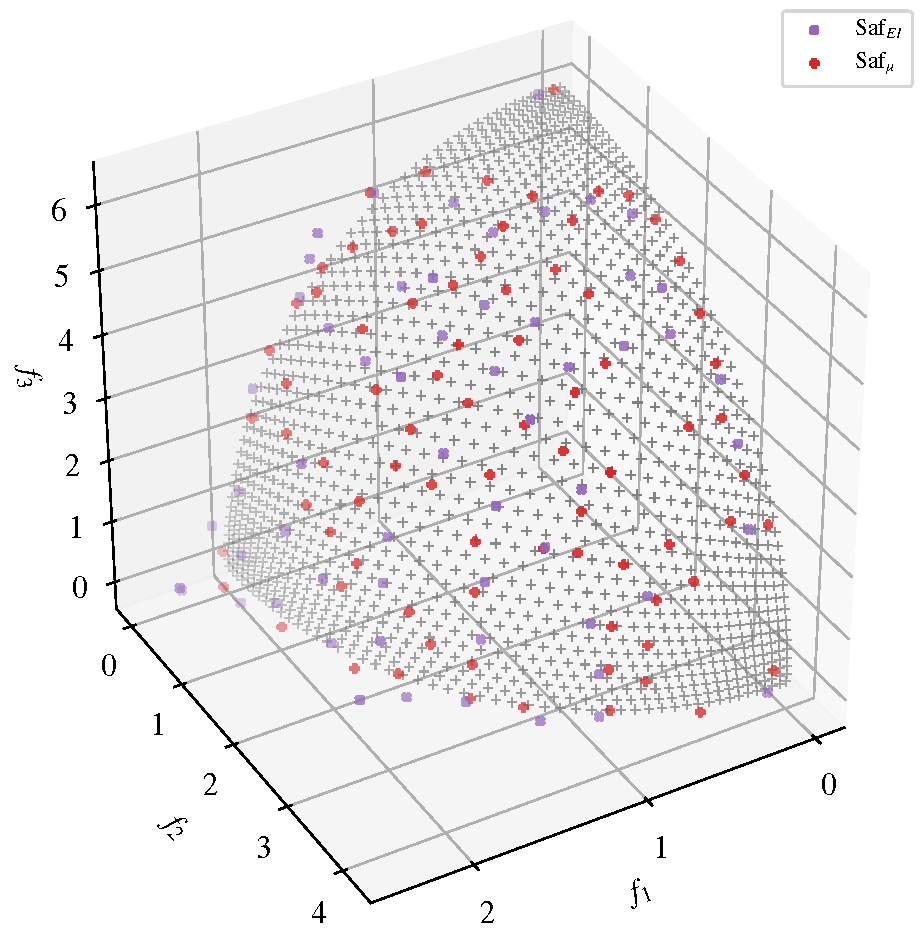
\includegraphics[width=0.6\linewidth]{figures/_comparison_attainmenPoints_safei_safmu.pdf}
\end{subfigure}
\begin{subfigure}[hbt!]{\linewidth}
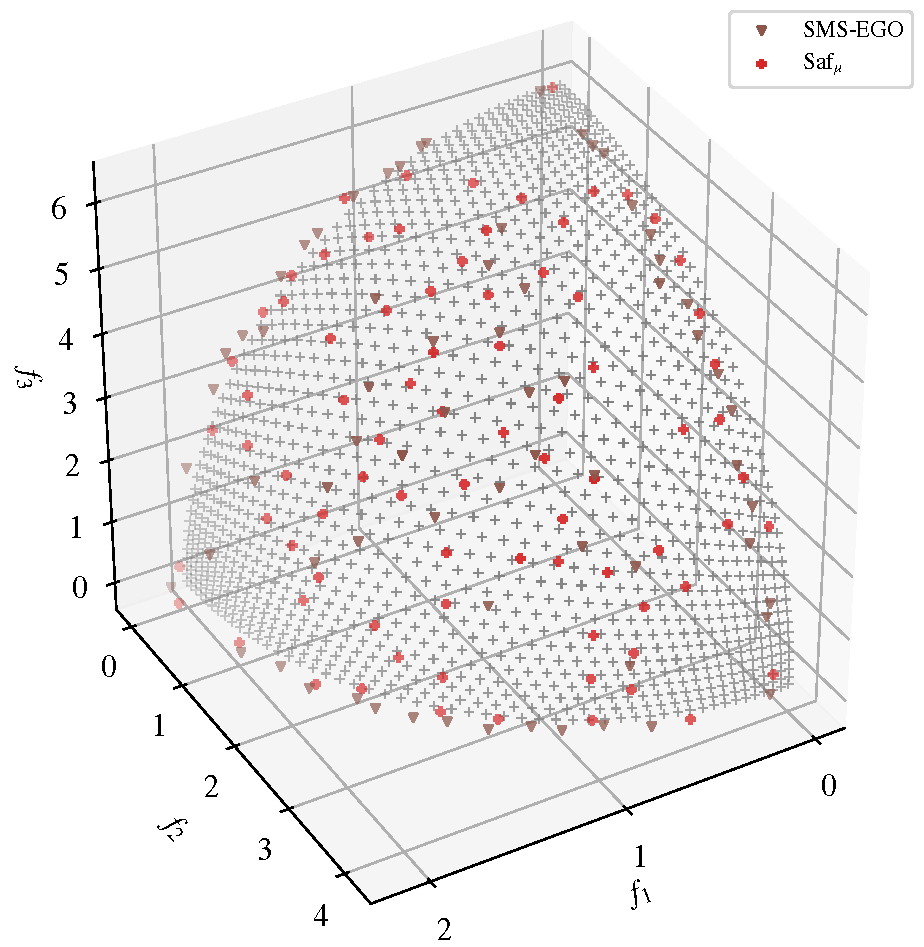
\includegraphics[width=0.6\linewidth]{figures/_comparison_attainmenPoints_sms_saf.pdf}
\end{subfigure}
\caption{Example of found solutions on WFG5 with $M=3$, $d=8$. Comparison between SAF$_{EI}$ and -SAF$_{\mu}$ above, and SAF$_{\mu}$ and SMS-EGO below. Solutions found after 150 evaluations and with identical starting conditions.}
\end{figure*}

\begin{figure*}
WFG1\_2M\_3d

\begin{subfigure}[hbt!]{\linewidth}

    \centering
    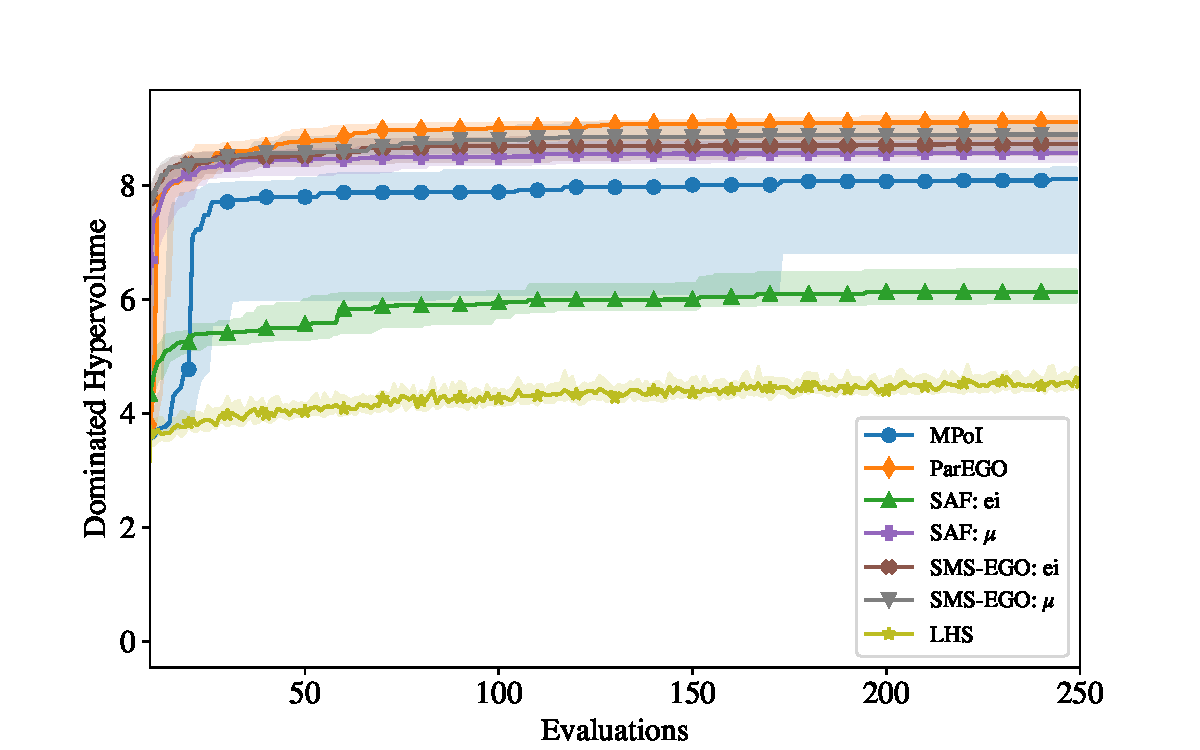
\includegraphics[width=0.7\linewidth]{figures/wfg1_2obj_3dim_hv_plot.pdf}
    % \caption{Caption}
\end{subfigure}
\begin{subfigure}[h]{\linewidth}
    \centering
    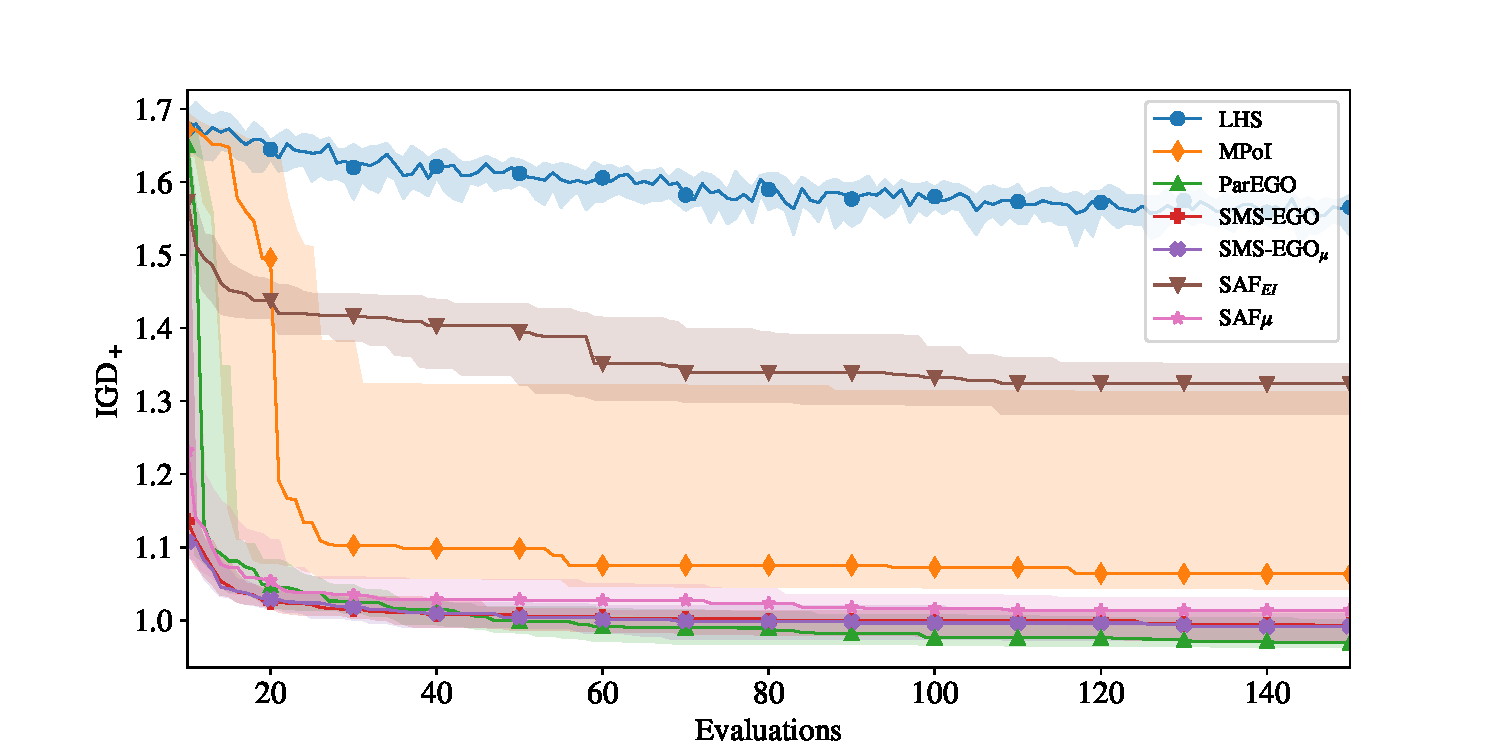
\includegraphics[width=0.7\linewidth]{figures/wfg1_2obj_3dim_igd_plot.pdf}
    % \caption{Caption}
\end{subfigure}
    \caption{Convergence plots showing median Dominated Hypervolume and IGD+ over 31 repeats. IQR shown in shaded region. Dominated hypervolume calculated as a fraction of the maximum possible.}
\vspace{\floatsep}
\begin{subfigure}[t]{\linewidth}
    \centering
    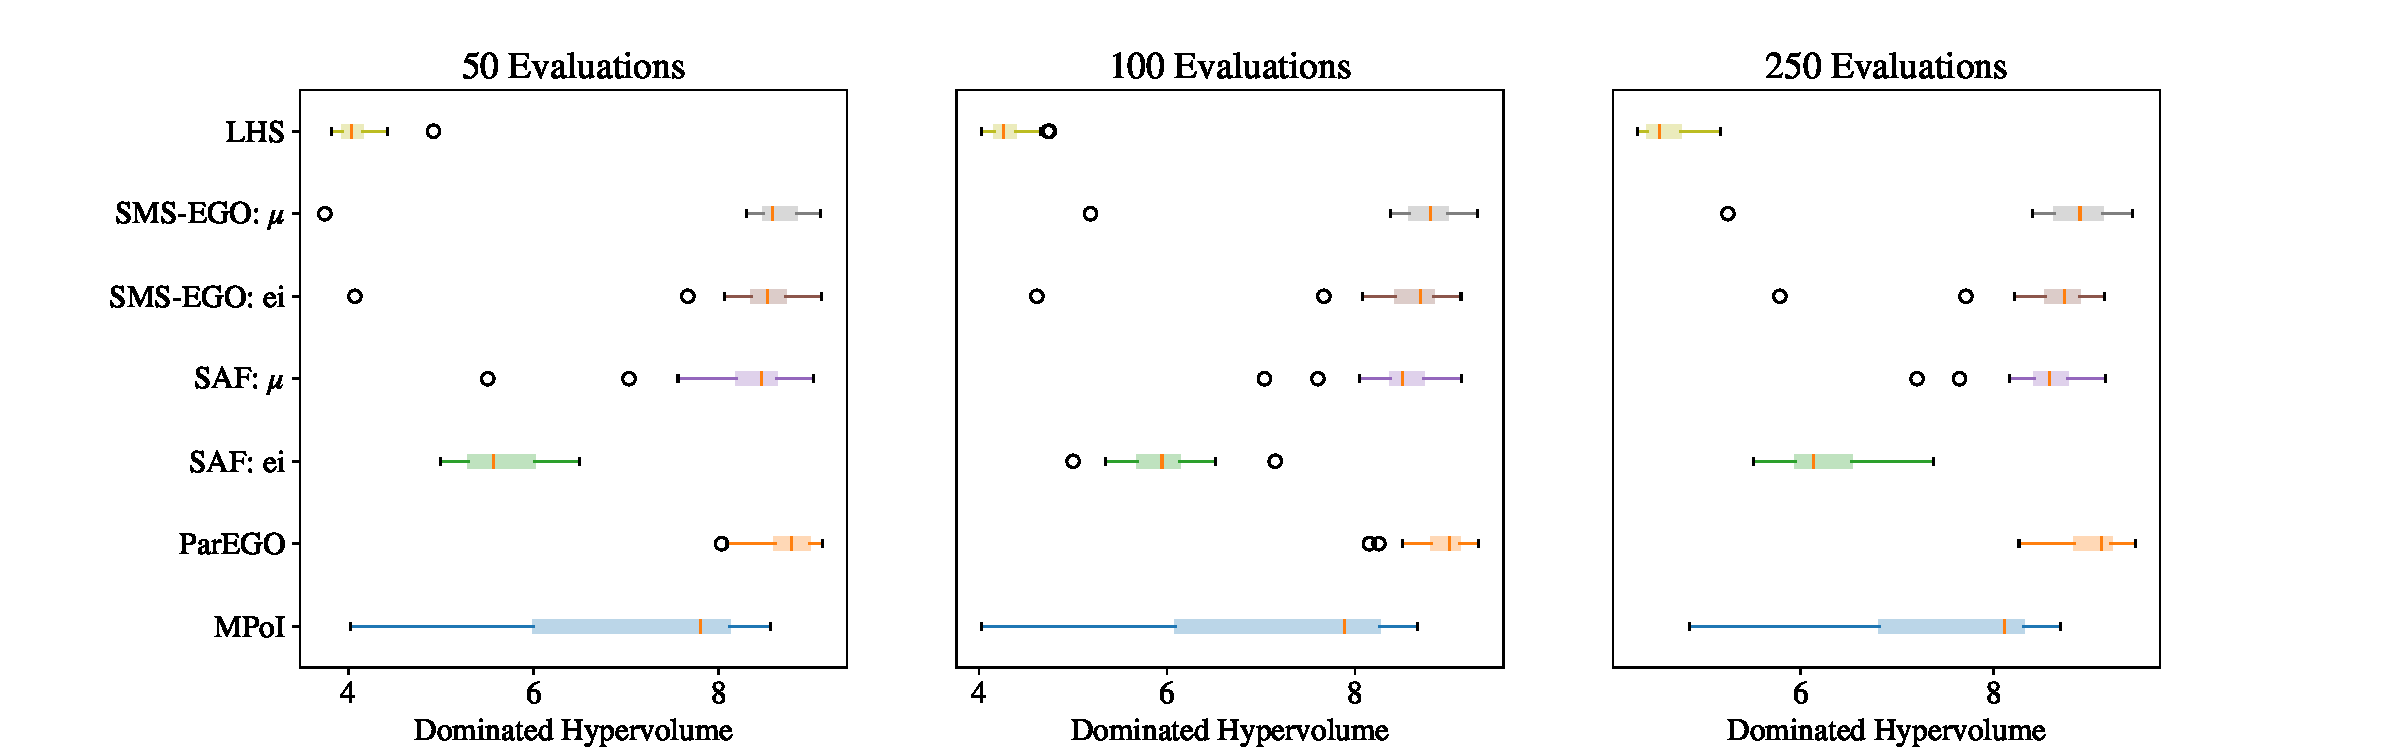
\includegraphics[width=0.8\linewidth]{figures/wfg1_2obj_3dim_hv_boxplot.pdf}
    % \caption{Caption}
\end{subfigure}
\begin{subfigure}[t]{\linewidth}
    \centering
    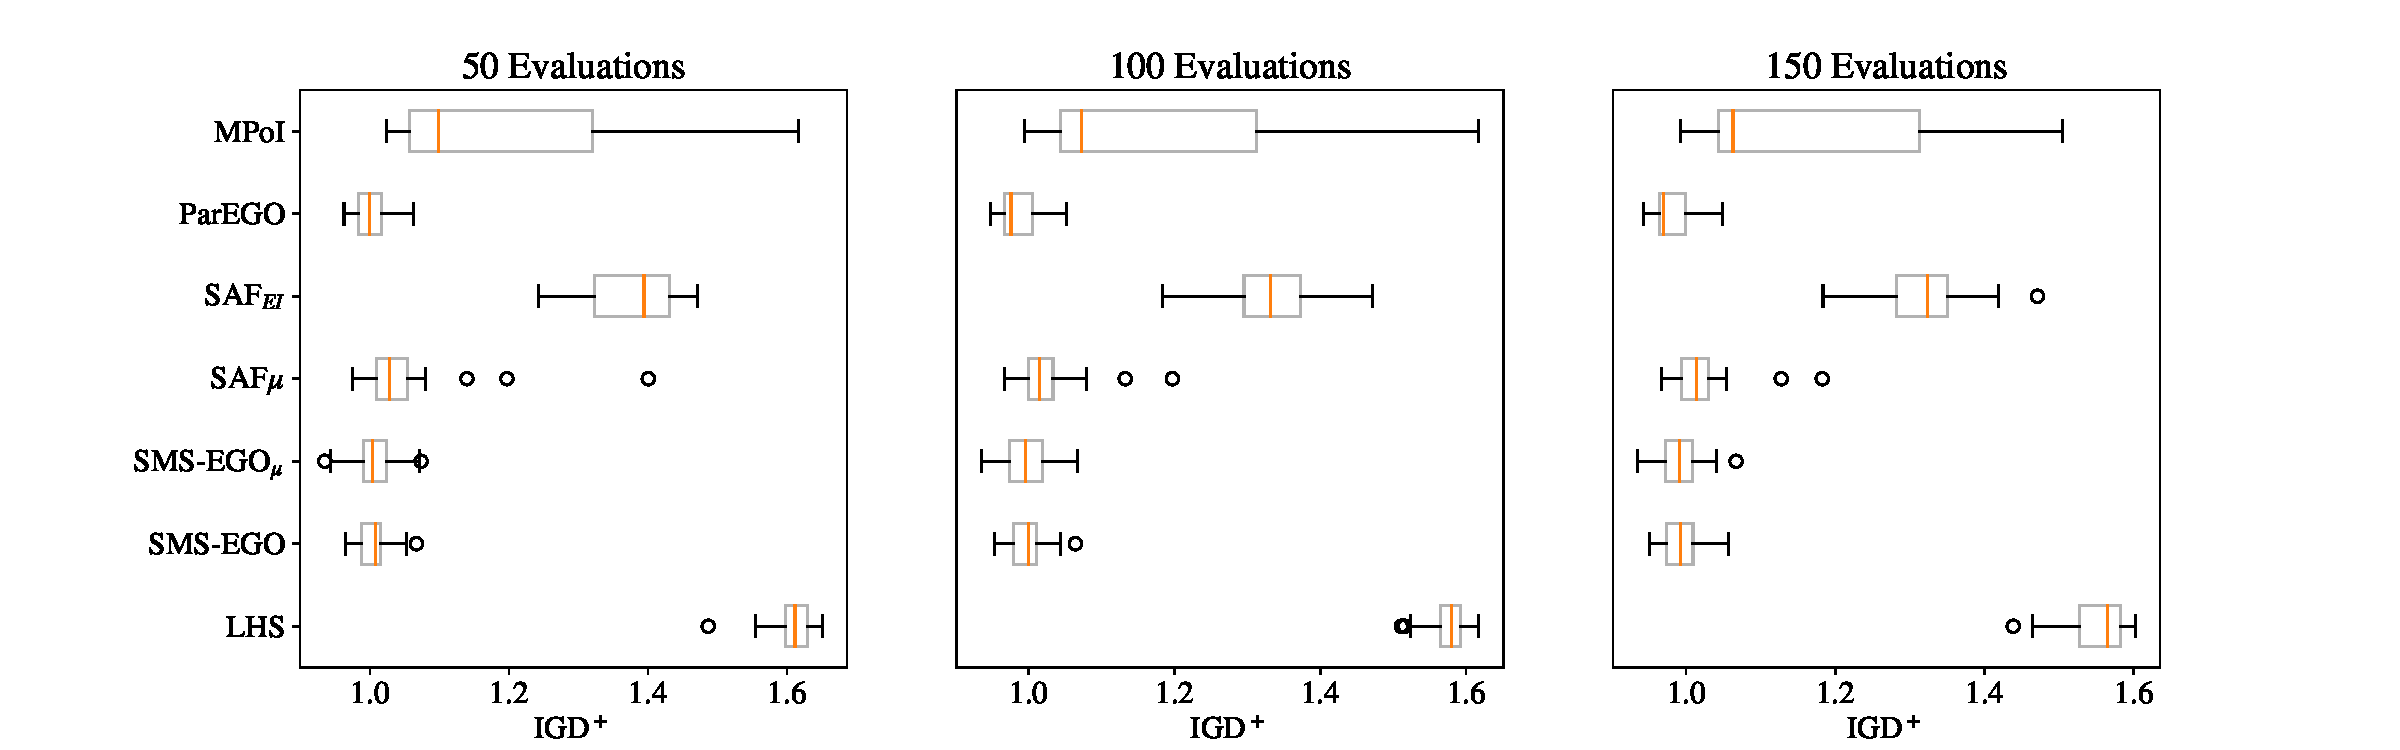
\includegraphics[width=0.8\linewidth]{figures/wfg1_2obj_3dim_igd_boxplot.pdf}
    % \caption{Caption}
\end{subfigure}
    \caption{Box plots showing Dominated Hypervolume and IGD+ over 31 repeats at three stages of the optimisation process.}
\end{figure*}
\clearpage



\begin{figure*}
WFG1\_3M\_4d

\begin{subfigure}[hbt!]{\linewidth}

    \centering
    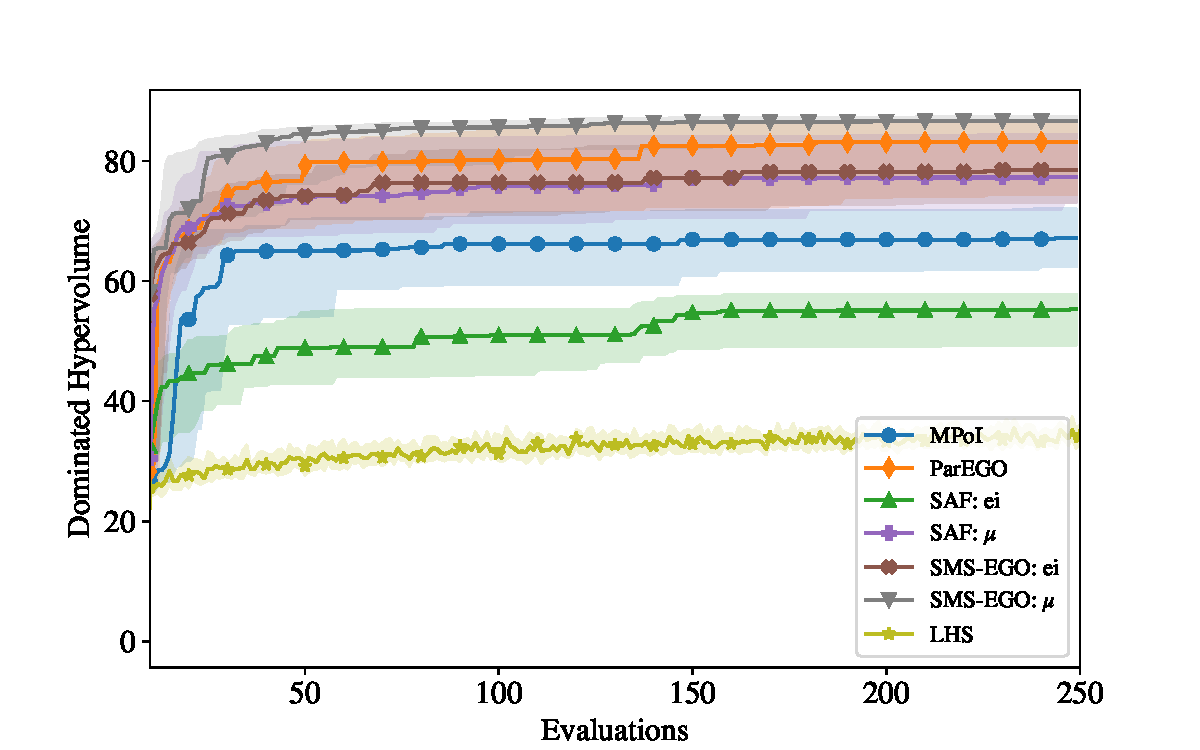
\includegraphics[width=0.7\linewidth]{figures/wfg1_3obj_4dim_hv_plot.pdf}
    % \caption{Caption}
\end{subfigure}
\begin{subfigure}[h]{\linewidth}
    \centering
    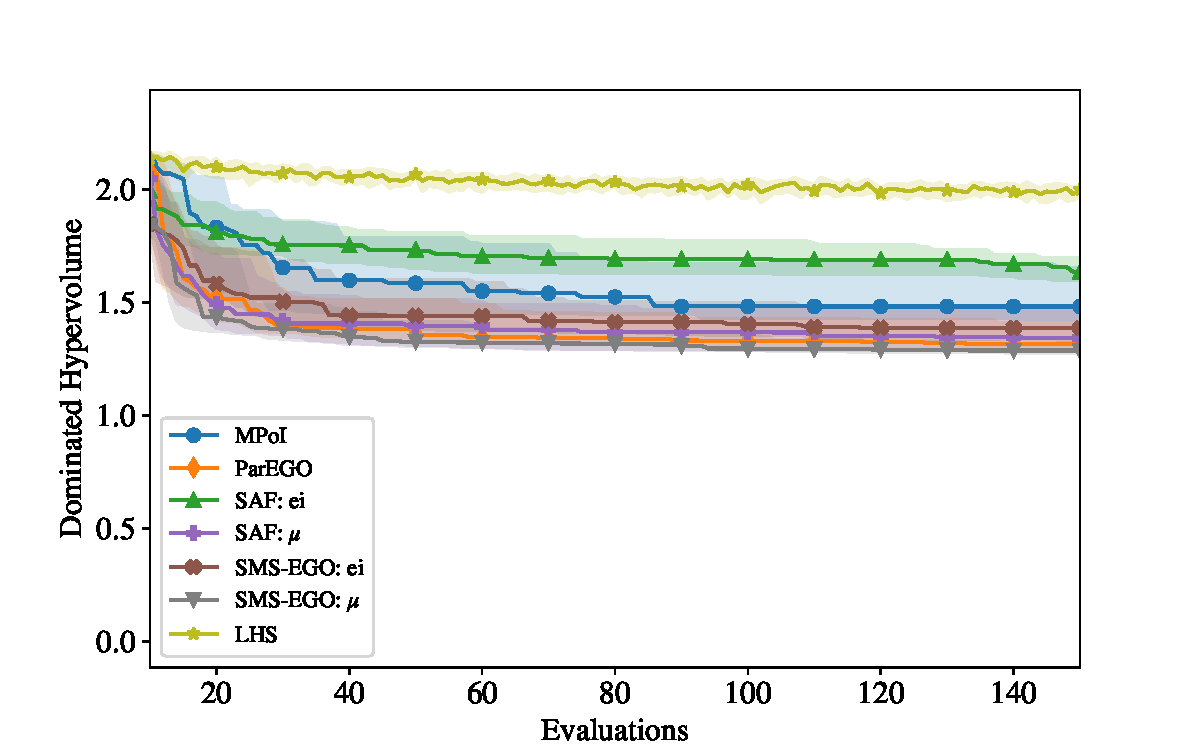
\includegraphics[width=0.7\linewidth]{figures/wfg1_3obj_4dim_igd_plot.pdf}
    % \caption{Caption}
\end{subfigure}
    \caption{Convergence plots showing median Dominated Hypervolume and IGD+ over 31 repeats. IQR shown in shaded region. Dominated hypervolume calculated as a fraction of the maximum possible.}
\vspace{\floatsep}
\begin{subfigure}[t]{\linewidth}
    \centering
    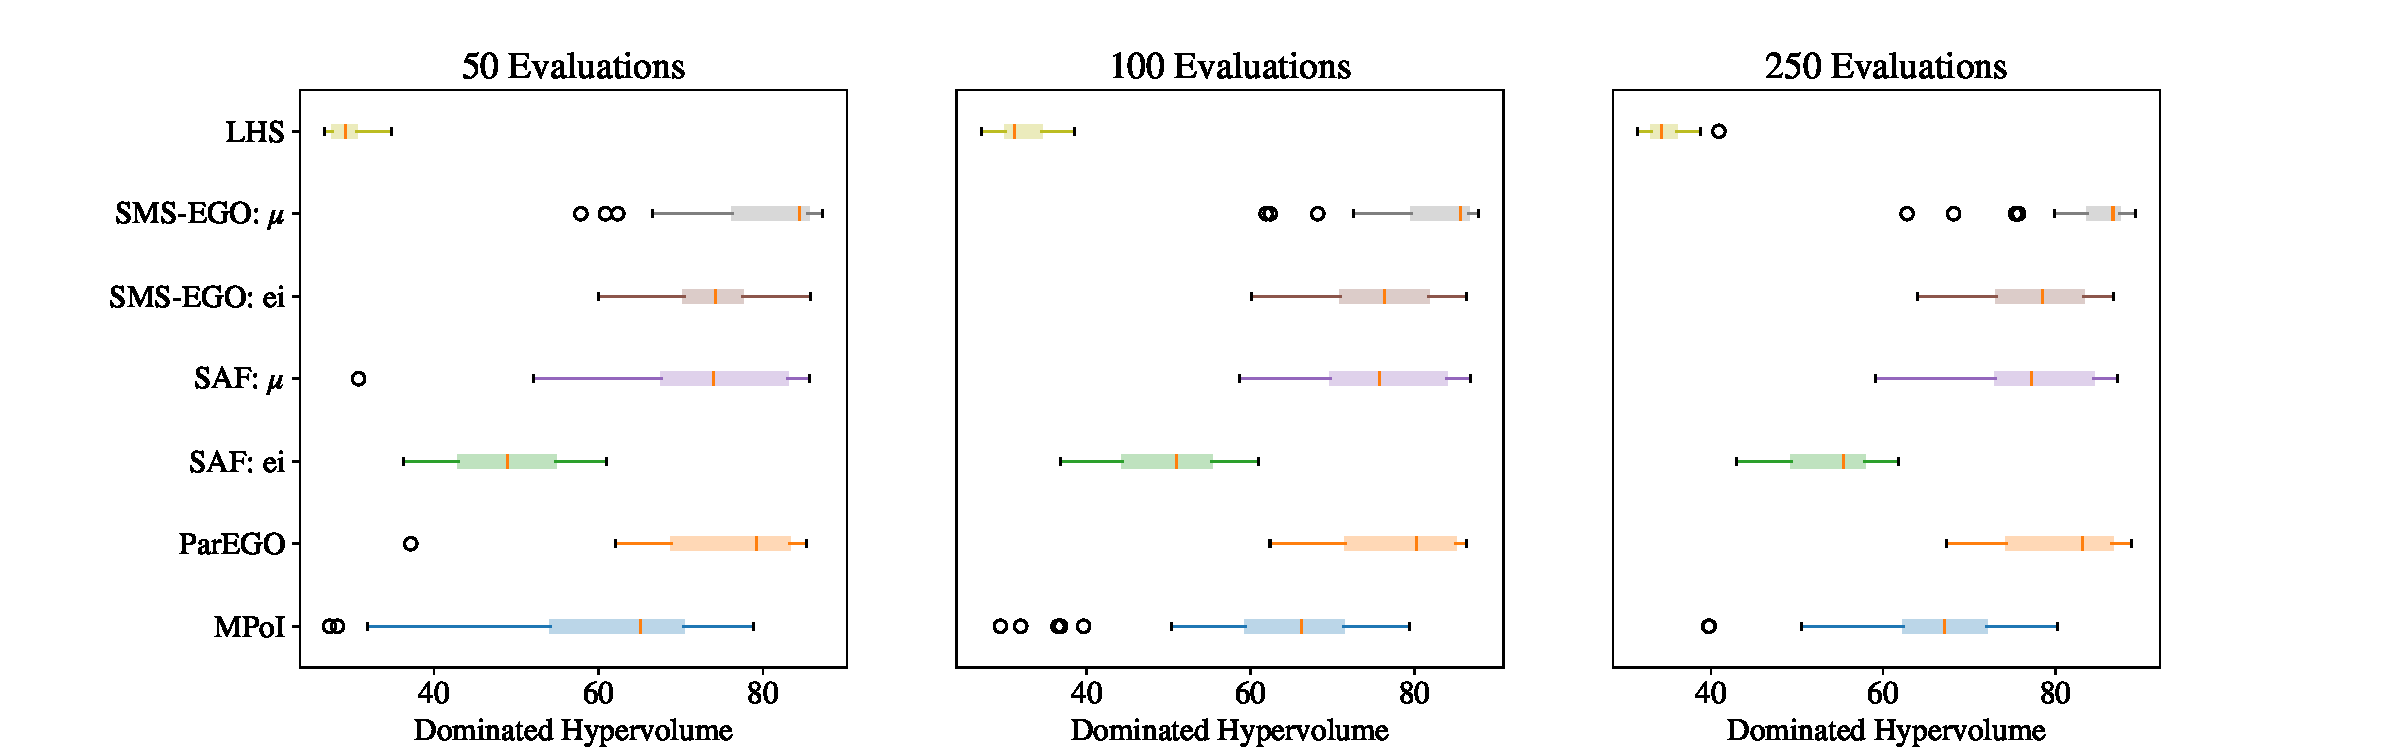
\includegraphics[width=0.8\linewidth]{figures/wfg1_3obj_4dim_hv_boxplot.pdf}
    % \caption{Caption}
\end{subfigure}
\begin{subfigure}[t]{\linewidth}
    \centering
    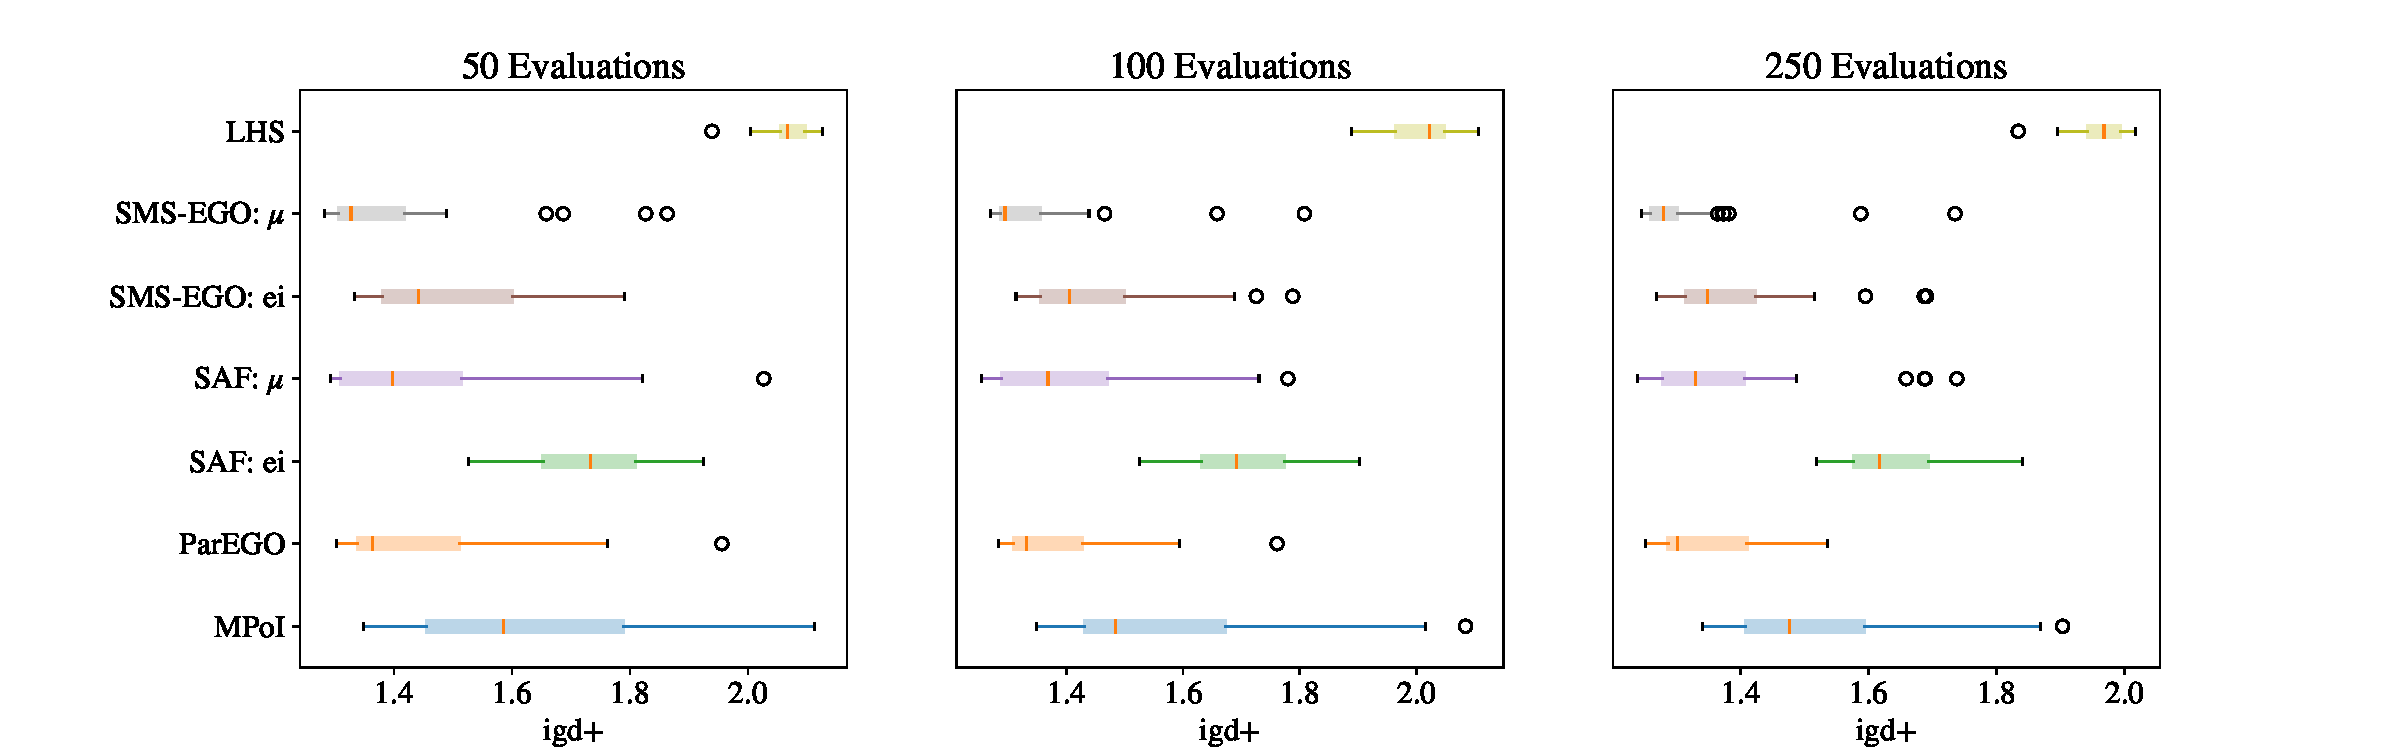
\includegraphics[width=0.8\linewidth]{figures/wfg1_3obj_4dim_igd_boxplot.pdf}
    % \caption{Caption}
\end{subfigure}
    \caption{Box plots showing Dominated Hypervolume and IGD+ over 31 repeats at three stages of the optimisation process.}
\end{figure*}
\clearpage


\begin{figure*}
WFG1\_4M\_5d


\begin{subfigure}[hbt!]{\linewidth}

    \centering
    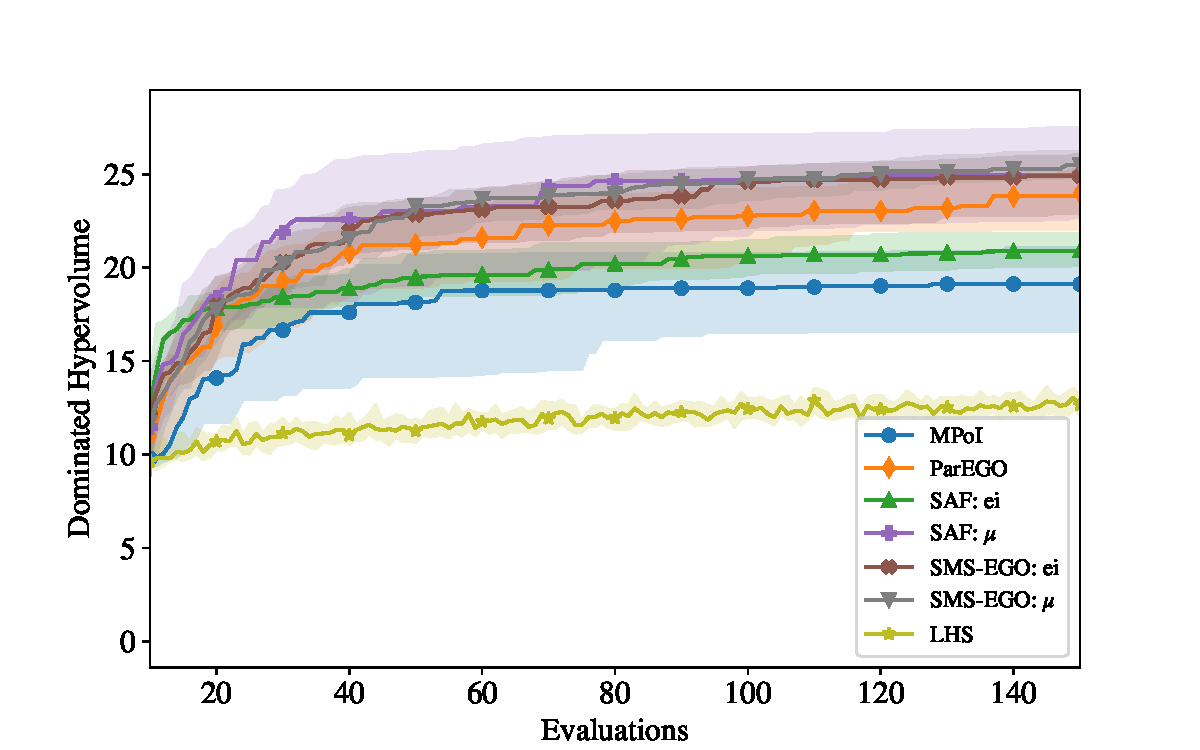
\includegraphics[width=0.7\linewidth]{figures/wfg1_4obj_5dim_hv_plot.pdf}
    % \caption{Caption}
\end{subfigure}
\begin{subfigure}[h]{\linewidth}
    \centering
    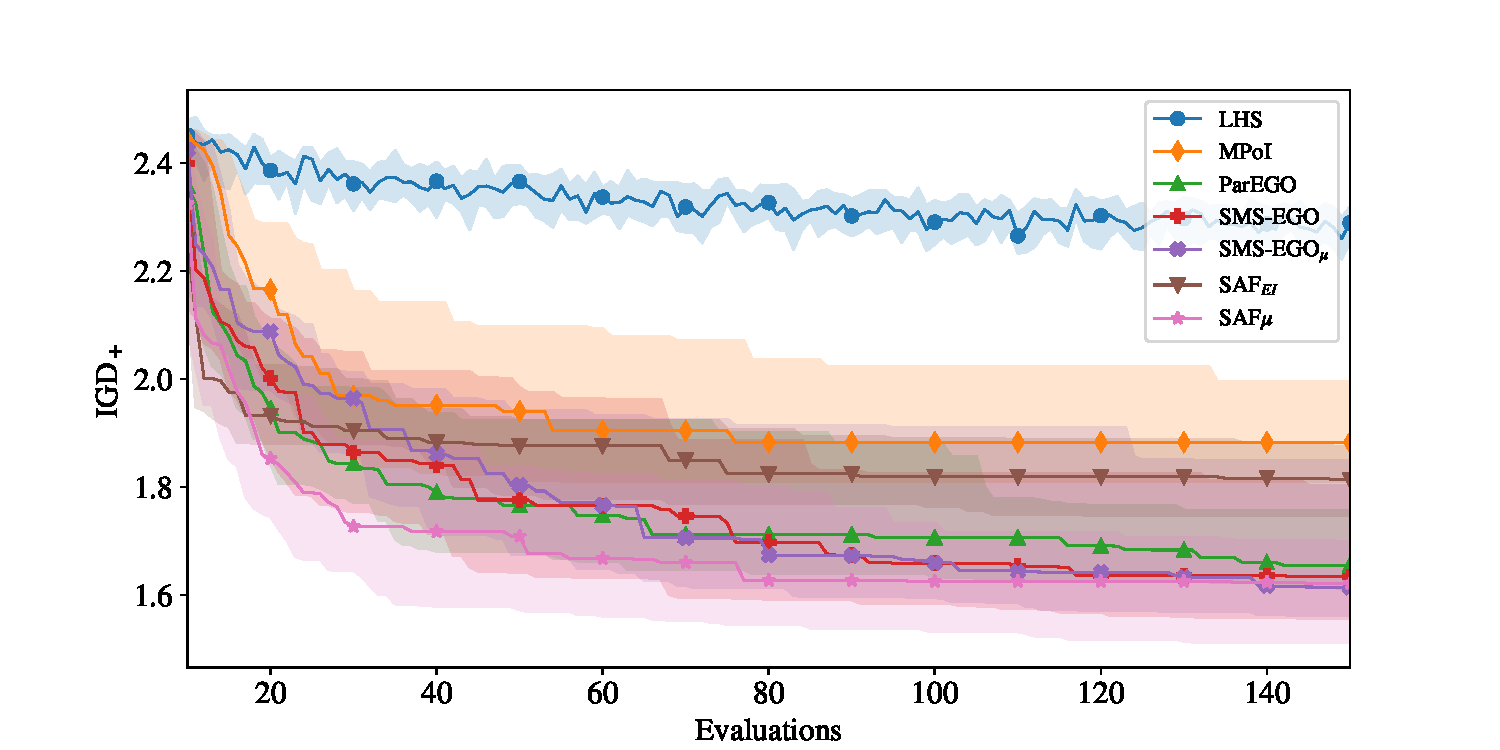
\includegraphics[width=0.7\linewidth]{figures/wfg1_4obj_5dim_igd_plot.pdf}
    % \caption{Caption}
\end{subfigure}
    \caption{Convergence plots showing median Dominated Hypervolume and IGD+ over 31 repeats. IQR shown in shaded region. Dominated hypervolume calculated as a fraction of the maximum possible.}
\vspace{\floatsep}
\begin{subfigure}[t]{\linewidth}
    \centering
    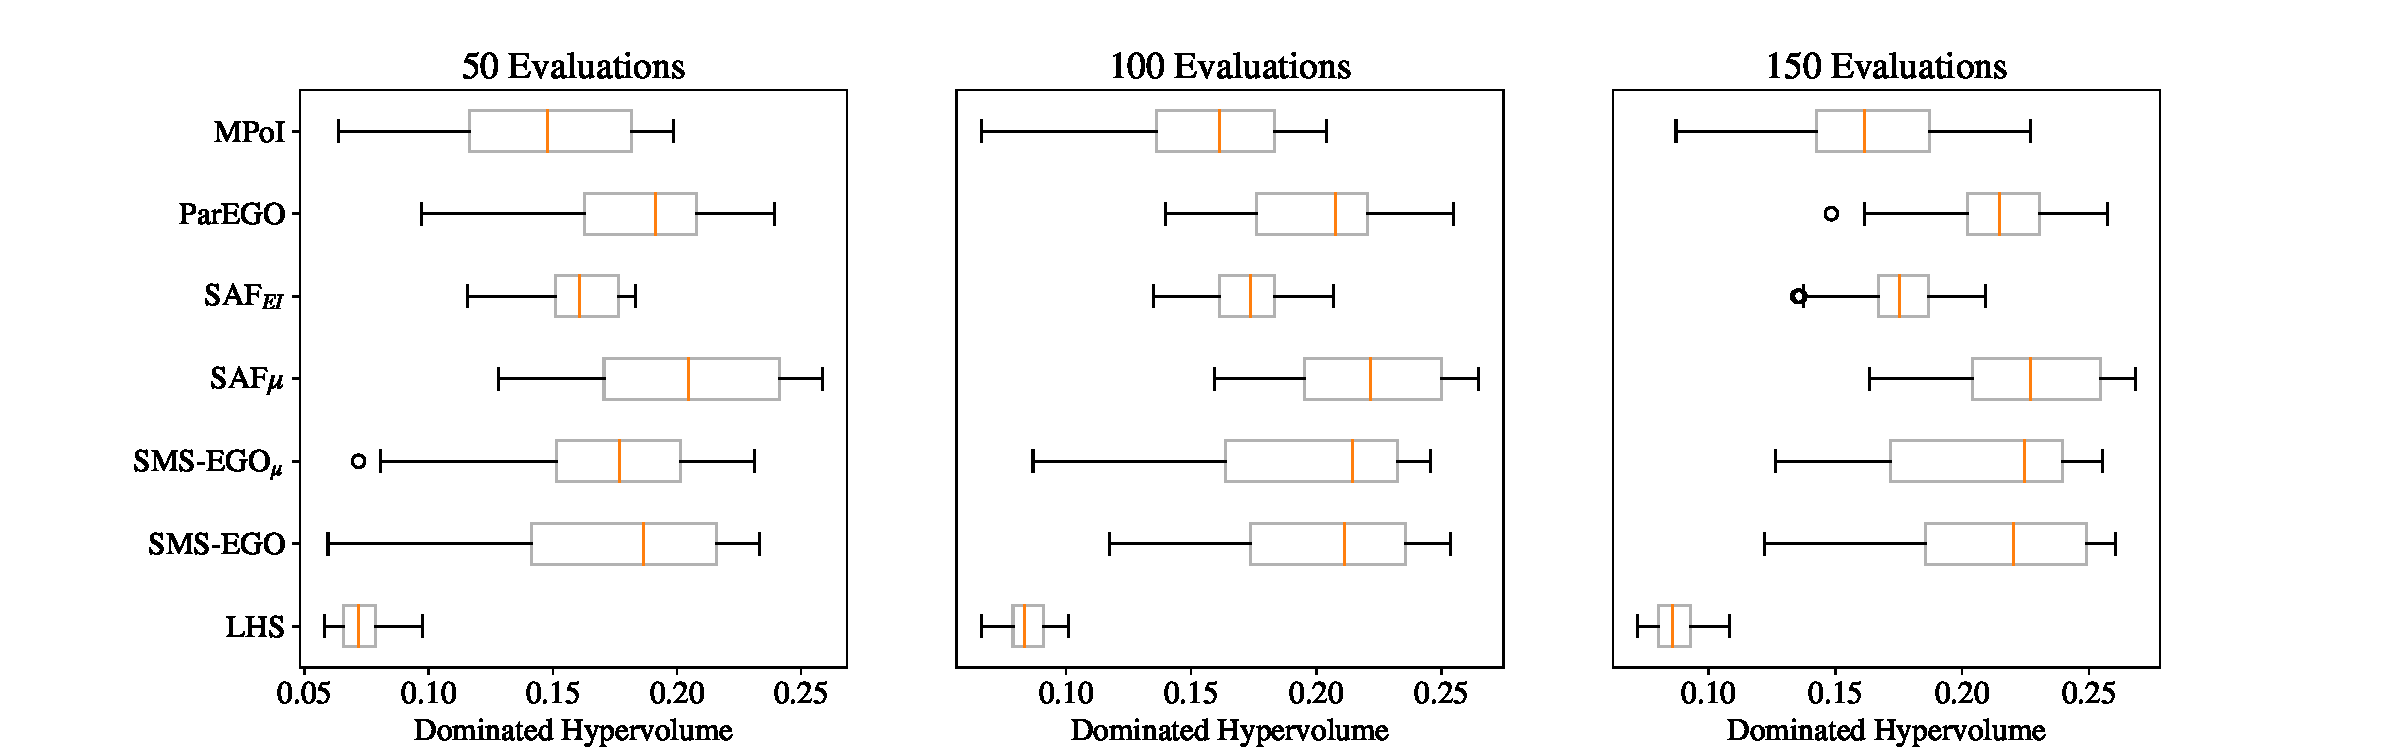
\includegraphics[width=0.8\linewidth]{figures/wfg1_4obj_5dim_hv_boxplot.pdf}
    % \caption{Caption}
\end{subfigure}
\begin{subfigure}[t]{\linewidth}
    \centering
    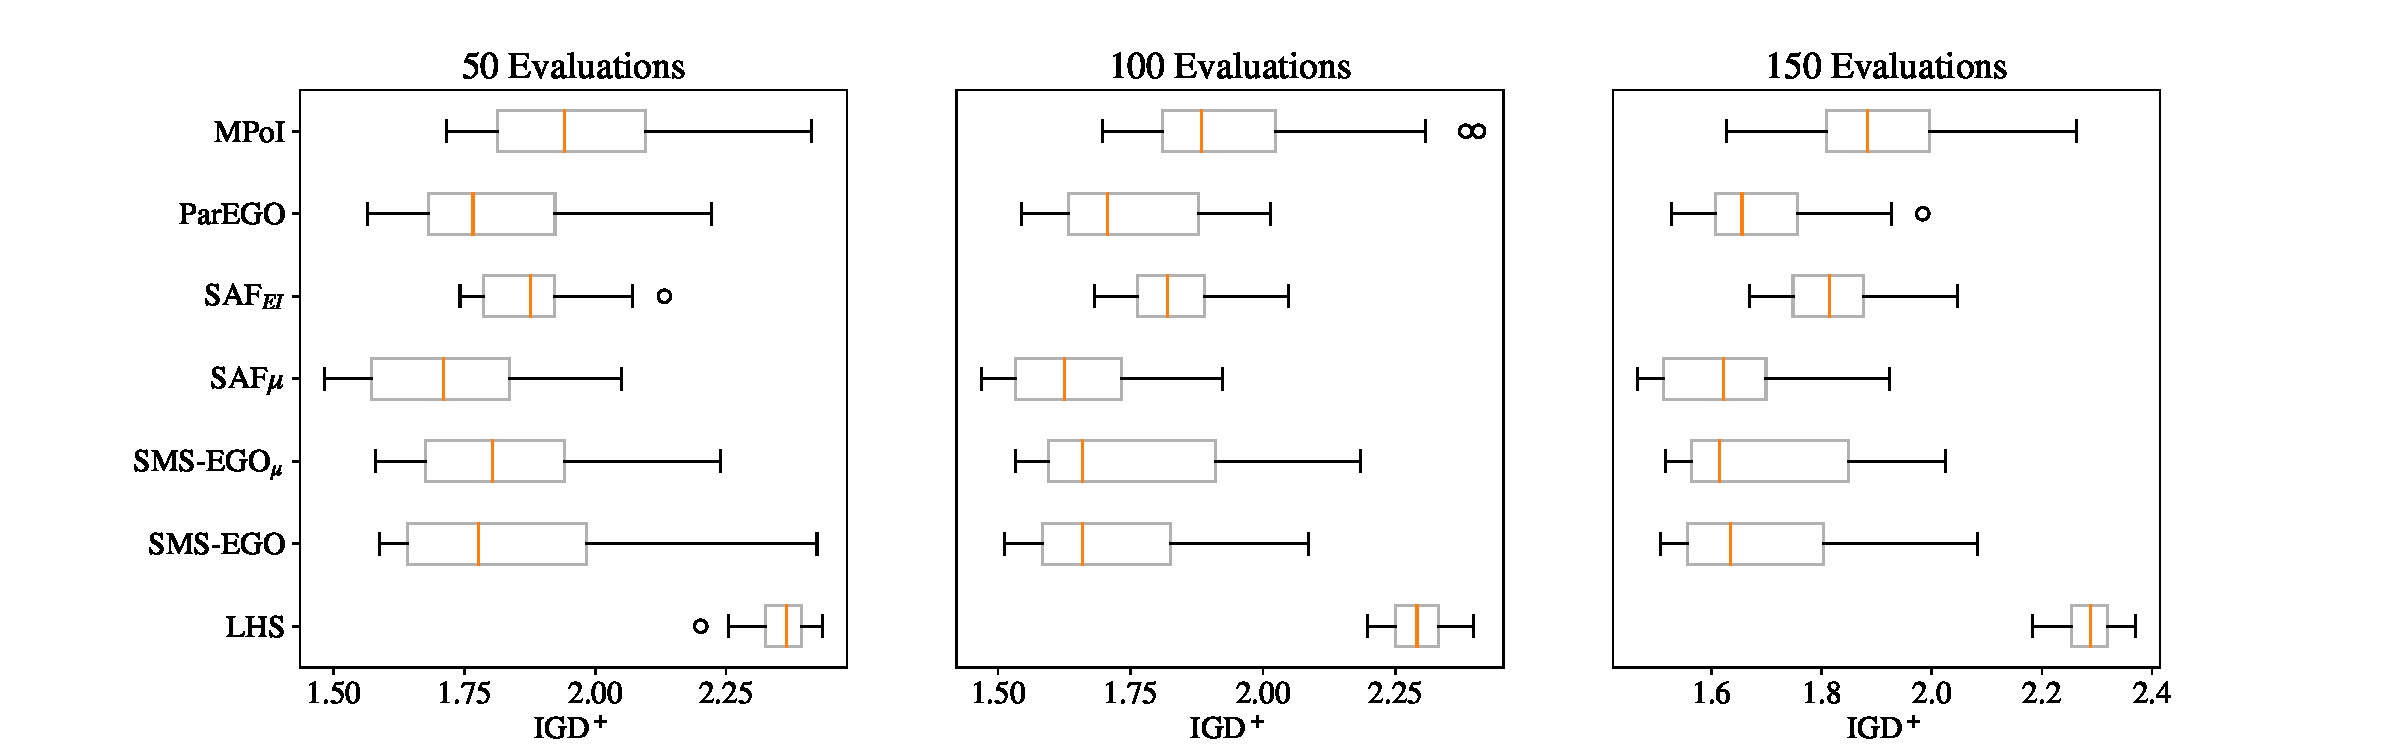
\includegraphics[width=0.8\linewidth]{figures/wfg1_4obj_5dim_igd_boxplot.pdf}
    % \caption{Caption}
\end{subfigure}
    \caption{Box plots showing Dominated Hypervolume and IGD+ over 31 repeats at three stages of the optimisation process.}
\end{figure*}
\clearpage


\begin{figure*}
WFG2\_2M\_6d


\begin{subfigure}[hbt!]{\linewidth}

    \centering
    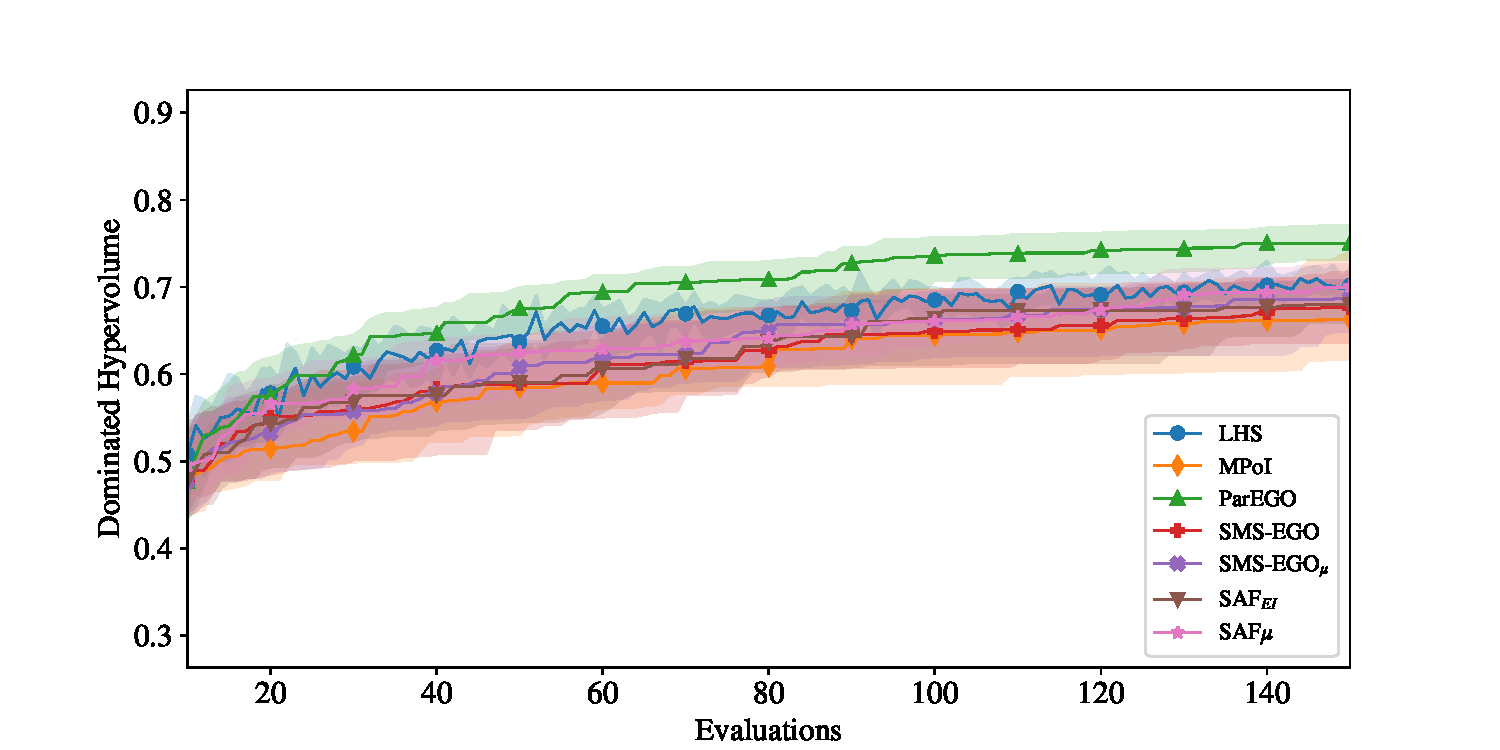
\includegraphics[width=0.7\linewidth]{figures/wfg2_2obj_6dim_hv_plot.pdf}
    % \caption{Caption}
\end{subfigure}
\begin{subfigure}[h]{\linewidth}
    \centering
    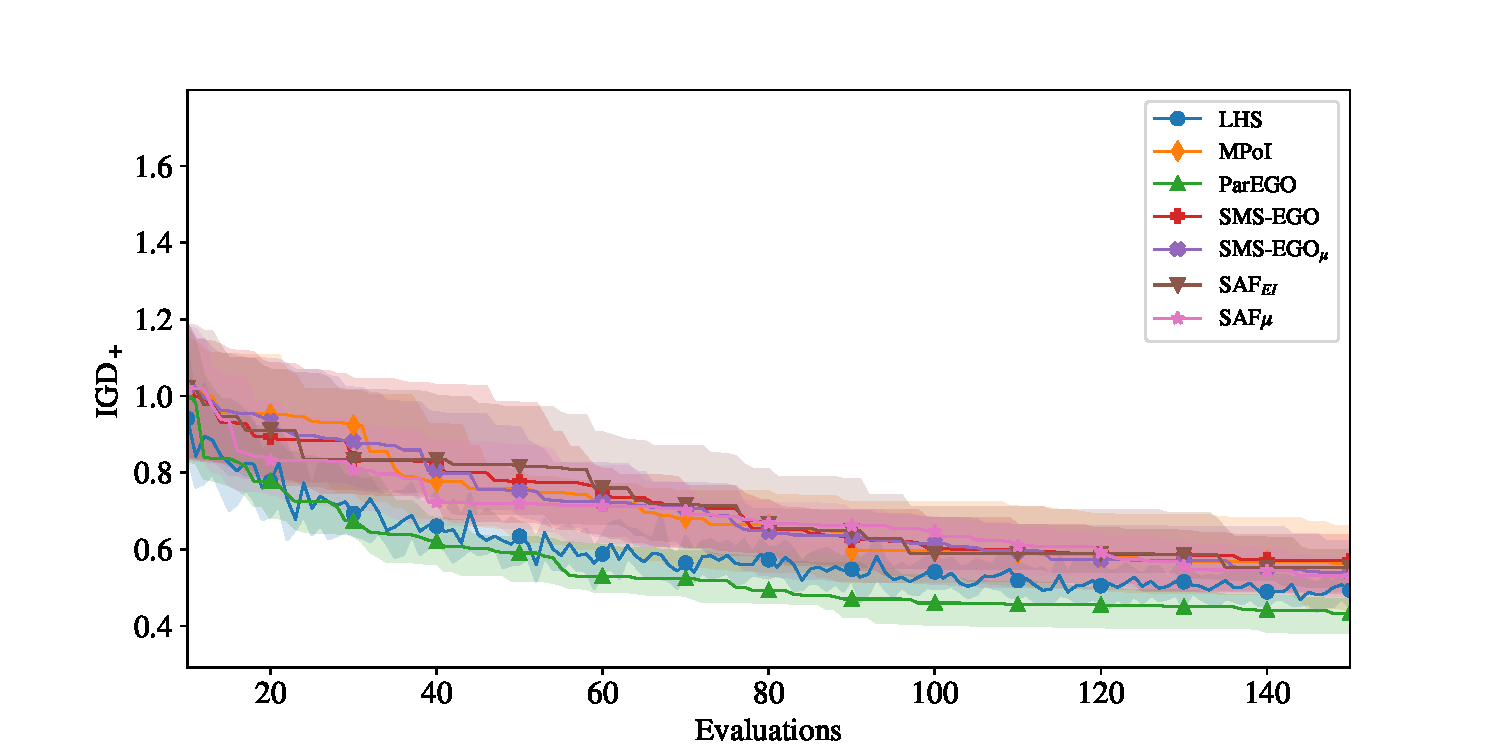
\includegraphics[width=0.7\linewidth]{figures/wfg2_2obj_6dim_igd_plot.pdf}
    % \caption{Caption}
\end{subfigure}
    \caption{Convergence plots showing median Dominated Hypervolume and IGD+ over 31 repeats. IQR shown in shaded region. Dominated hypervolume calculated as a fraction of the maximum possible.}
\vspace{\floatsep}
\begin{subfigure}[t]{\linewidth}
    \centering
    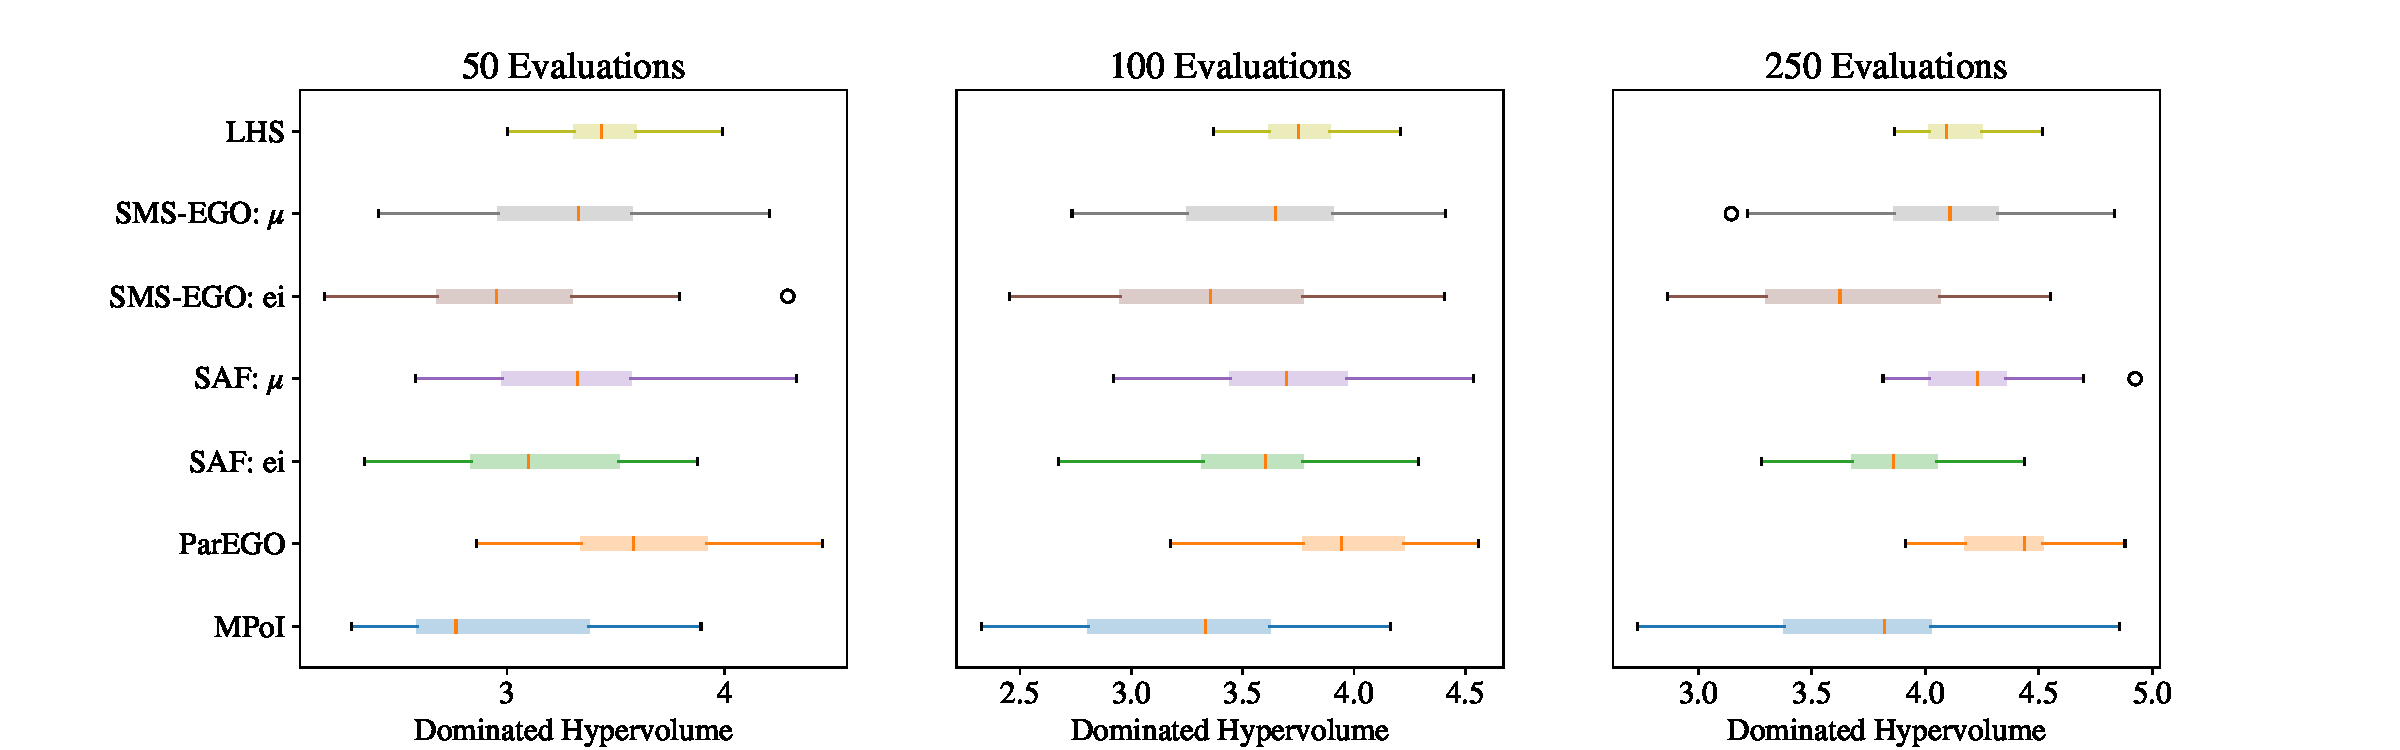
\includegraphics[width=0.8\linewidth]{figures/wfg2_2obj_6dim_hv_boxplot.pdf}
    % \caption{Caption}
\end{subfigure}
\begin{subfigure}[t]{\linewidth}
    \centering
    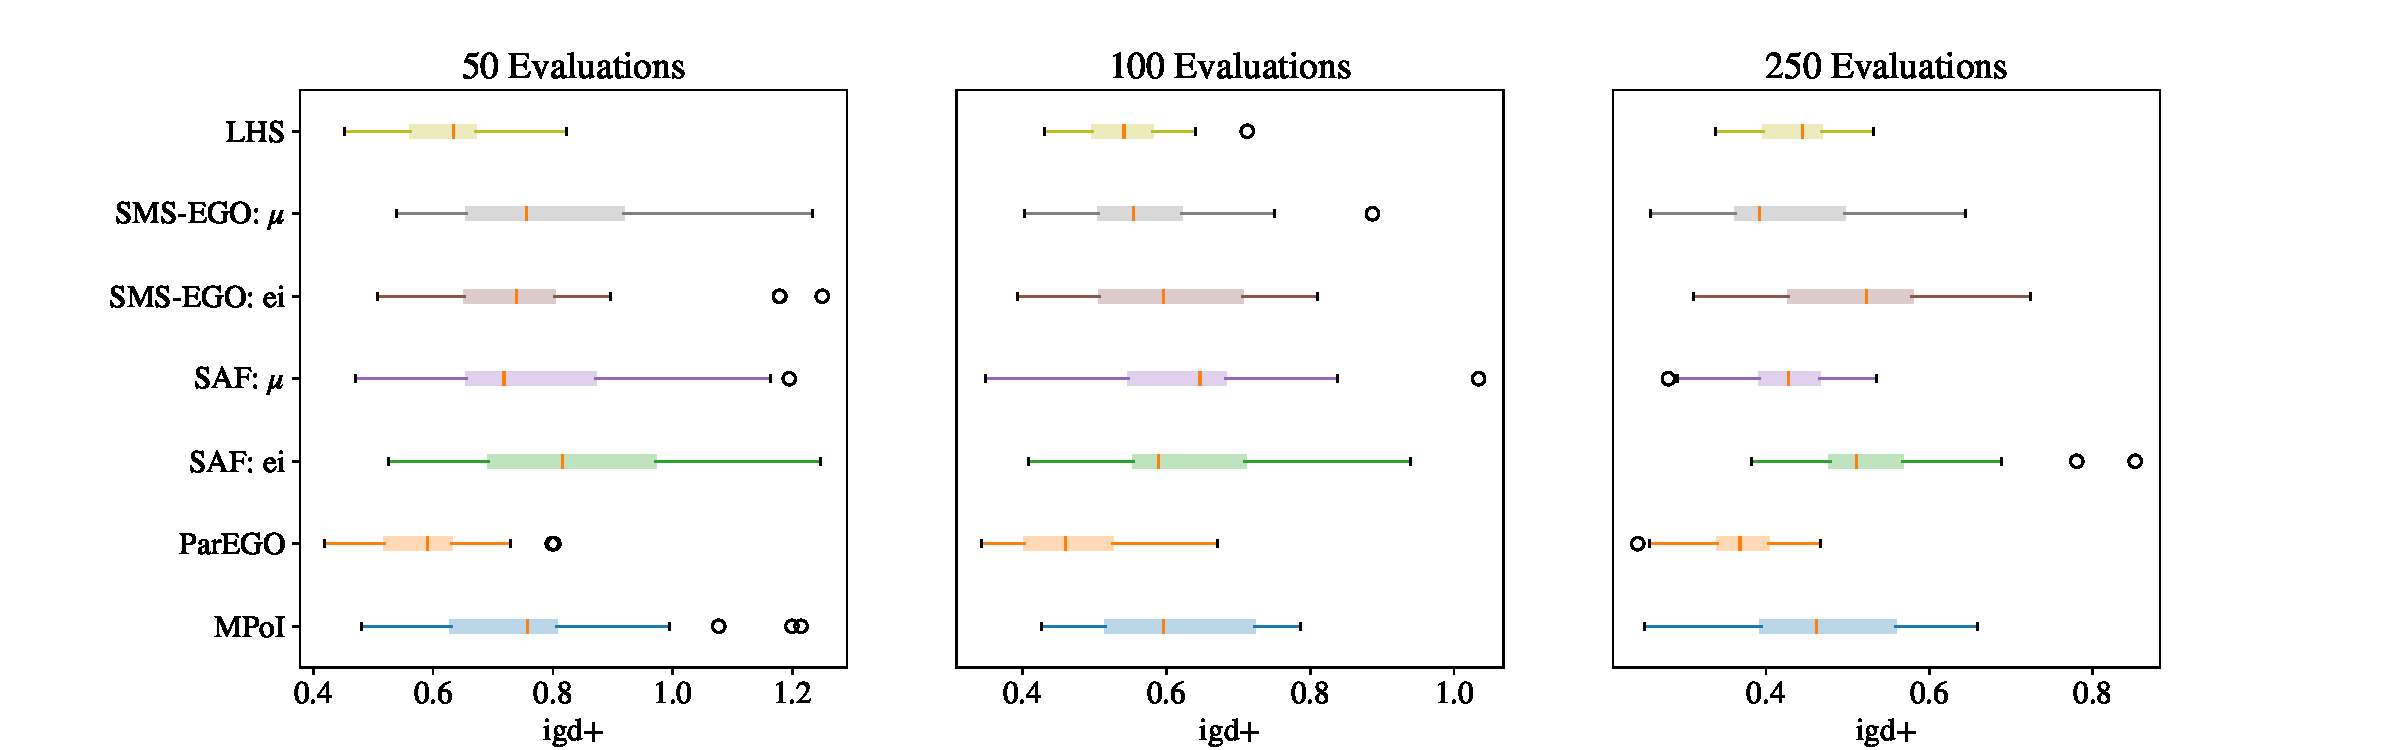
\includegraphics[width=0.8\linewidth]{figures/wfg2_2obj_6dim_igd_boxplot.pdf}
    % \caption{Caption}
\end{subfigure}
    \caption{Box plots showing Dominated Hypervolume and IGD+ over 31 repeats at three stages of the optimisation process.}
\end{figure*}
\clearpage

\begin{figure*}
WFG2\_3M\_6d


\begin{subfigure}[hbt!]{\linewidth}

    \centering
    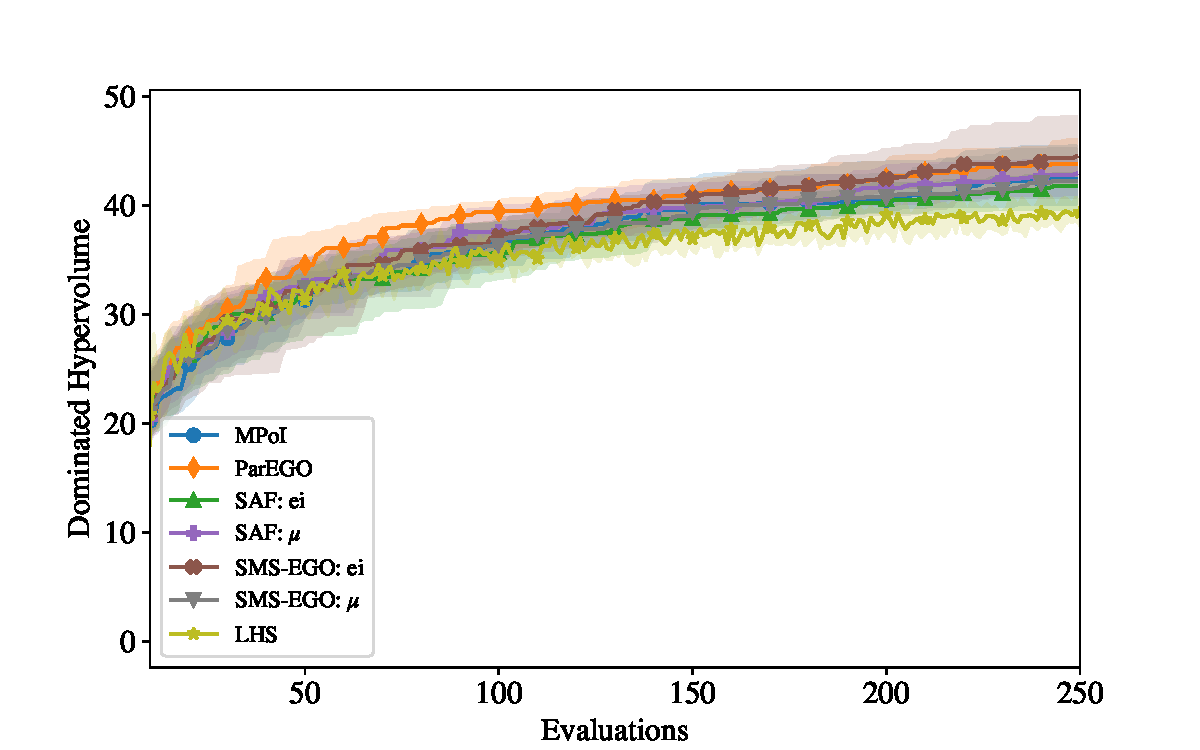
\includegraphics[width=0.7\linewidth]{figures/wfg2_3obj_6dim_hv_plot.pdf}
    % \caption{Caption}
\end{subfigure}
\begin{subfigure}[h]{\linewidth}
    \centering
    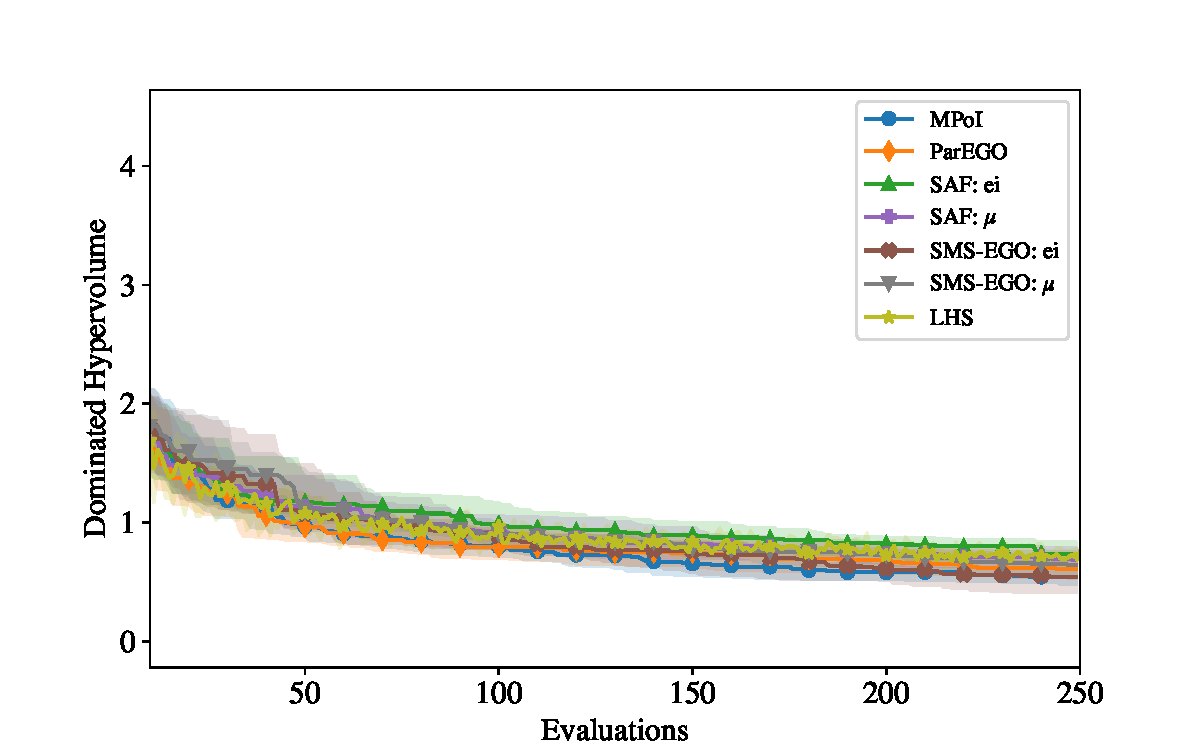
\includegraphics[width=0.7\linewidth]{figures/wfg2_3obj_6dim_igd_plot.pdf}
    % \caption{Caption}
\end{subfigure}
    \caption{Convergence plots showing median Dominated Hypervolume and IGD+ over 31 repeats. IQR shown in shaded region. Dominated hypervolume calculated as a fraction of the maximum possible.}
\vspace{\floatsep}
\begin{subfigure}[t]{\linewidth}
    \centering
    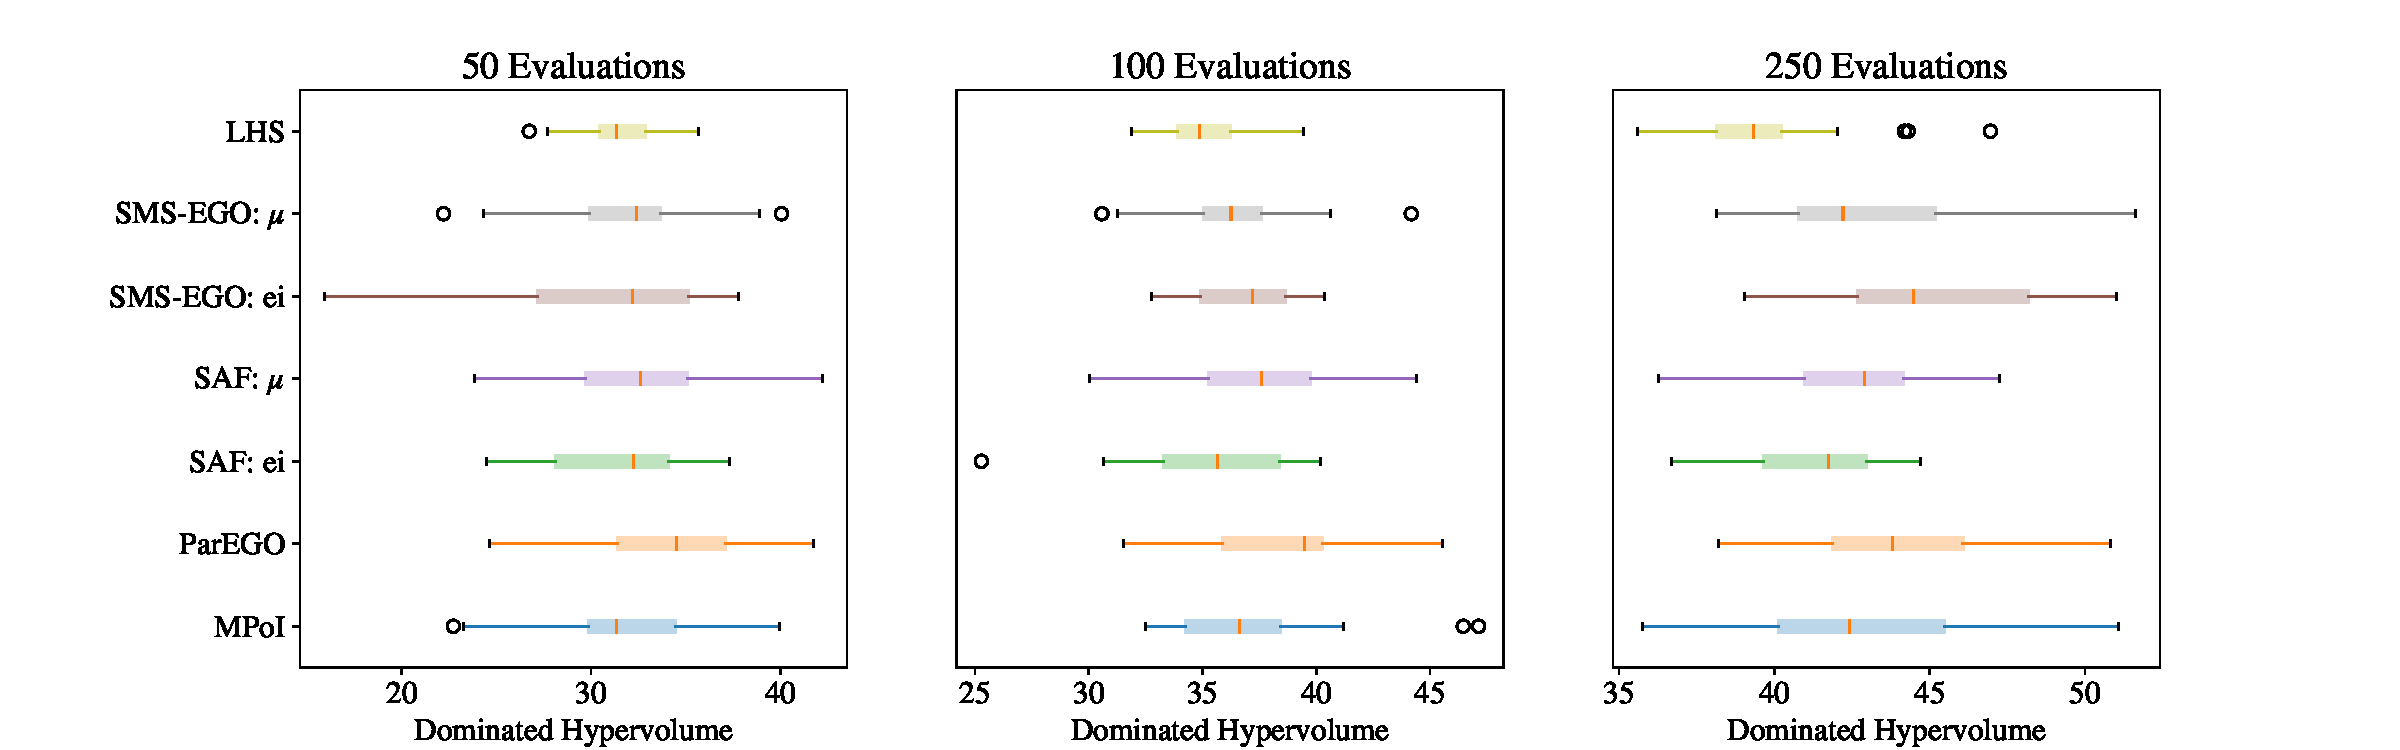
\includegraphics[width=0.8\linewidth]{figures/wfg2_3obj_6dim_hv_boxplot.pdf}
    % \caption{Caption}
\end{subfigure}
\begin{subfigure}[t]{\linewidth}
    \centering
    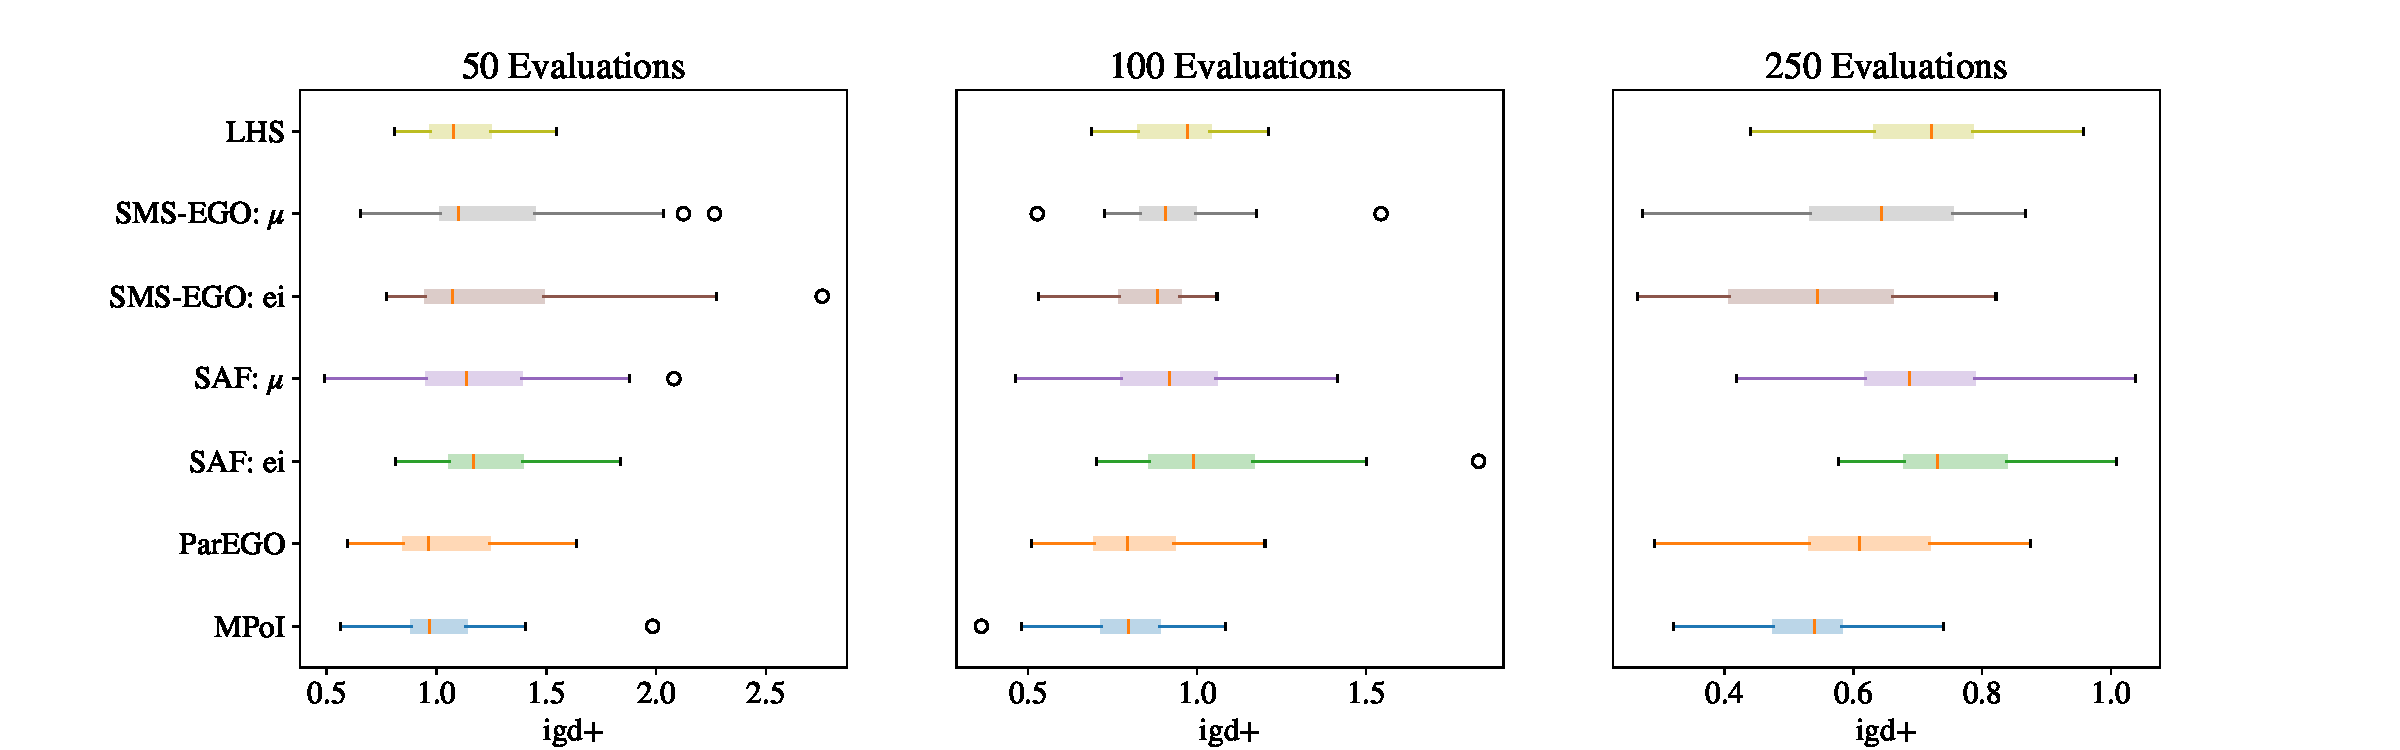
\includegraphics[width=0.8\linewidth]{figures/wfg2_3obj_6dim_igd_boxplot.pdf}
    % \caption{Caption}
\end{subfigure}
    \caption{Box plots showing Dominated Hypervolume and IGD+ over 31 repeats at three stages of the optimisation process.}
\end{figure*}

\clearpage

\begin{figure*}
WFG2\_4M\_10d


\begin{subfigure}[hbt!]{\linewidth}

    \centering
    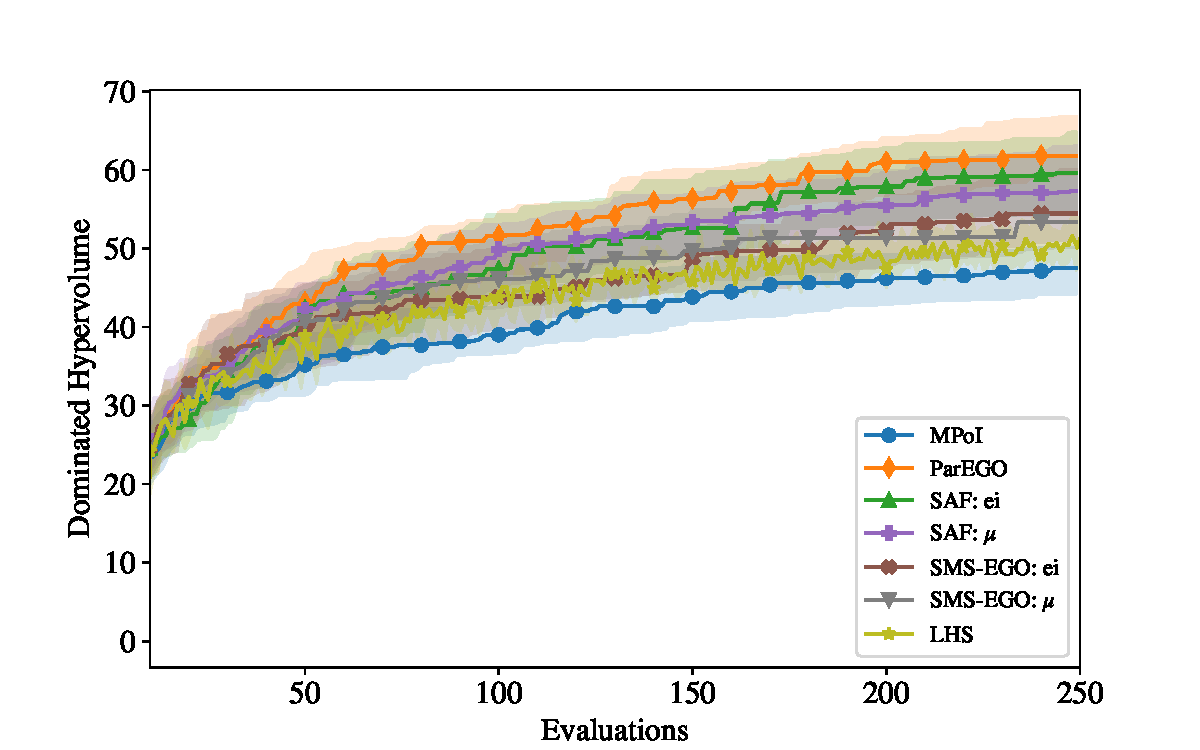
\includegraphics[width=0.7\linewidth]{figures/wfg2_4obj_10dim_hv_plot.pdf}
    % \caption{Caption}
\end{subfigure}
\begin{subfigure}[h]{\linewidth}
    \centering
    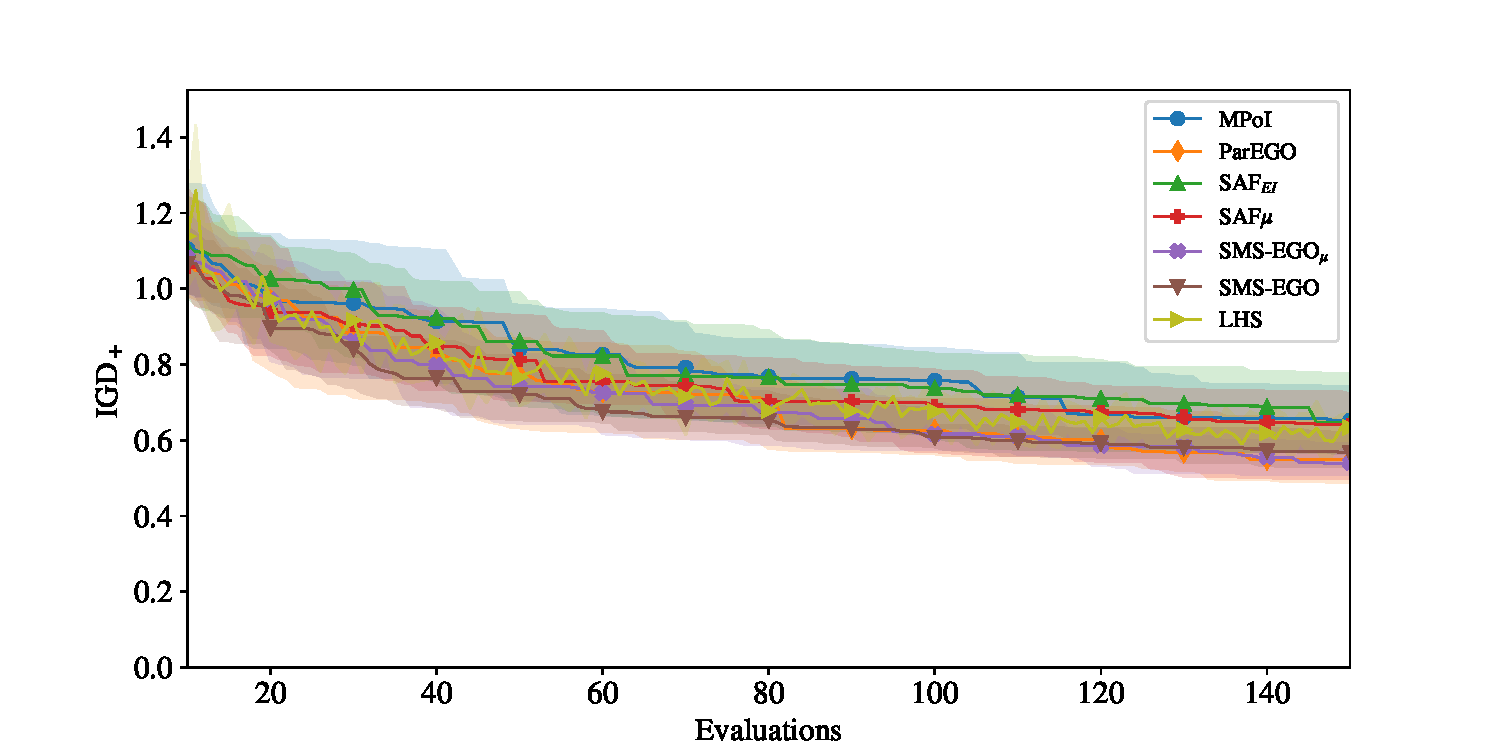
\includegraphics[width=0.7\linewidth]{figures/wfg2_4obj_10dim_igd_plot.pdf}
    % \caption{Caption}
\end{subfigure}
    \caption{Convergence plots showing median Dominated Hypervolume and IGD+ over 31 repeats. IQR shown in shaded region. Dominated hypervolume calculated as a fraction of the maximum possible.}
\vspace{\floatsep}
\begin{subfigure}[t]{\linewidth}
    \centering
    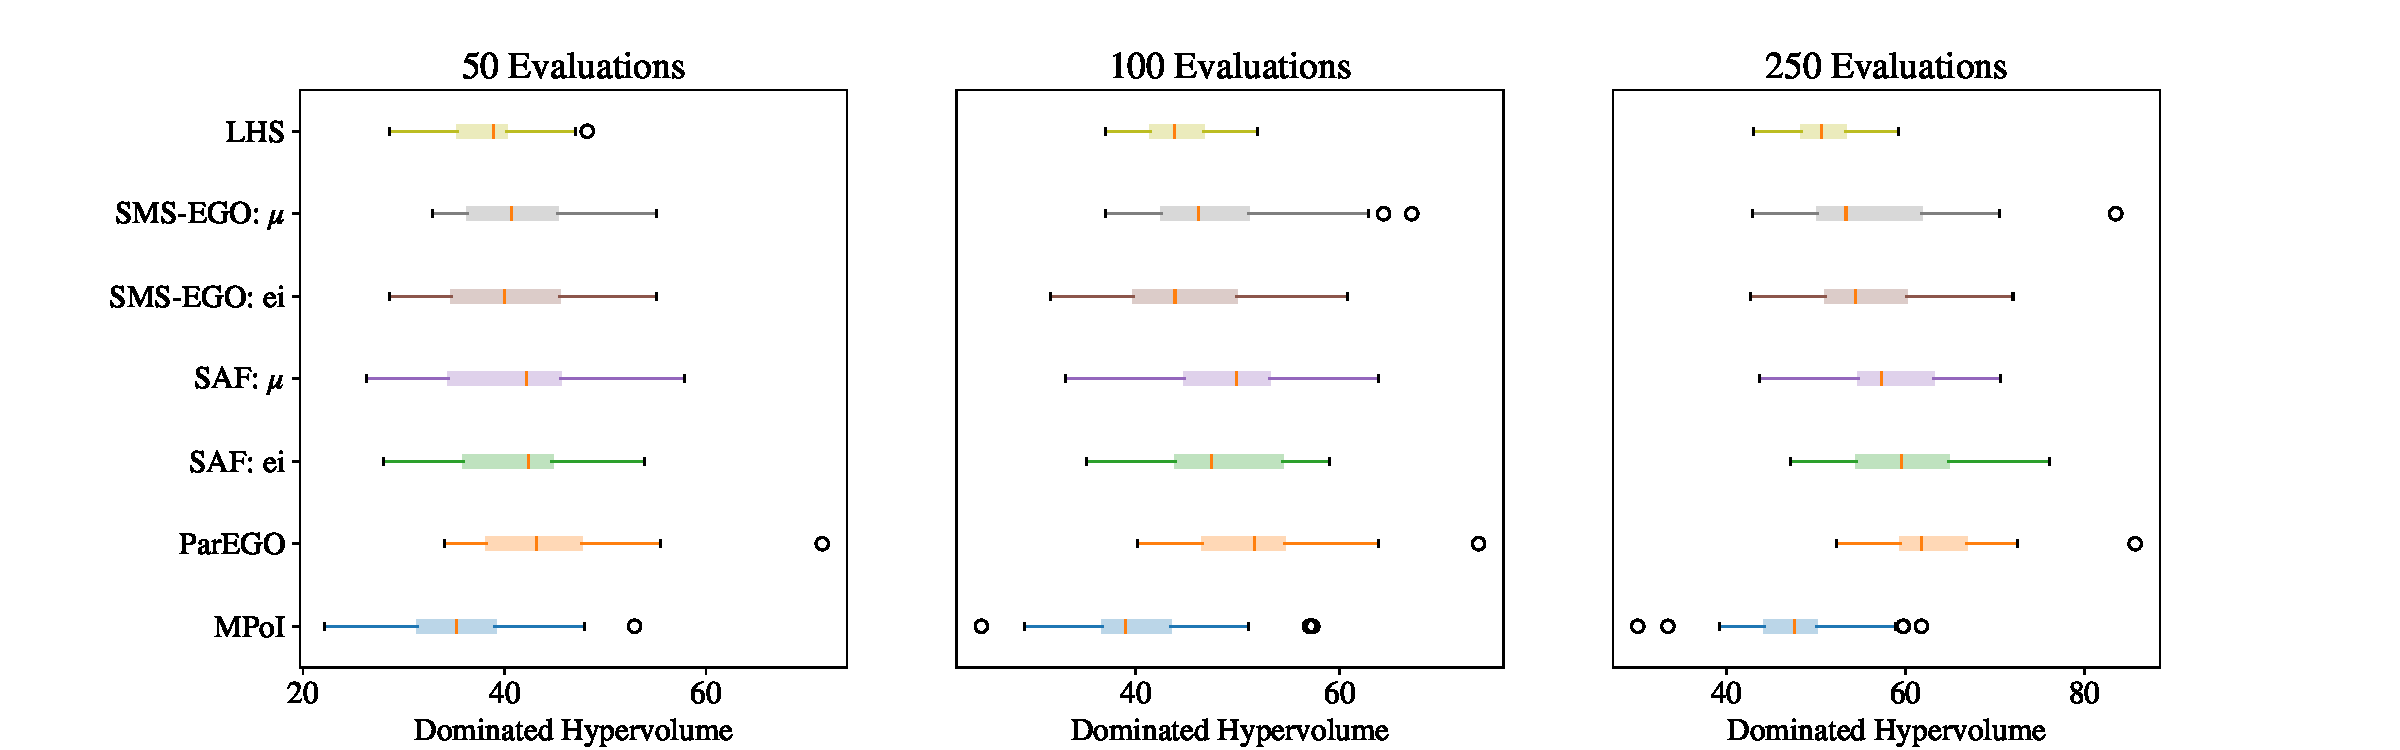
\includegraphics[width=0.8\linewidth]{figures/wfg2_4obj_10dim_hv_boxplot.pdf}
    % \caption{Caption}
\end{subfigure}
\begin{subfigure}[t]{\linewidth}
    \centering
    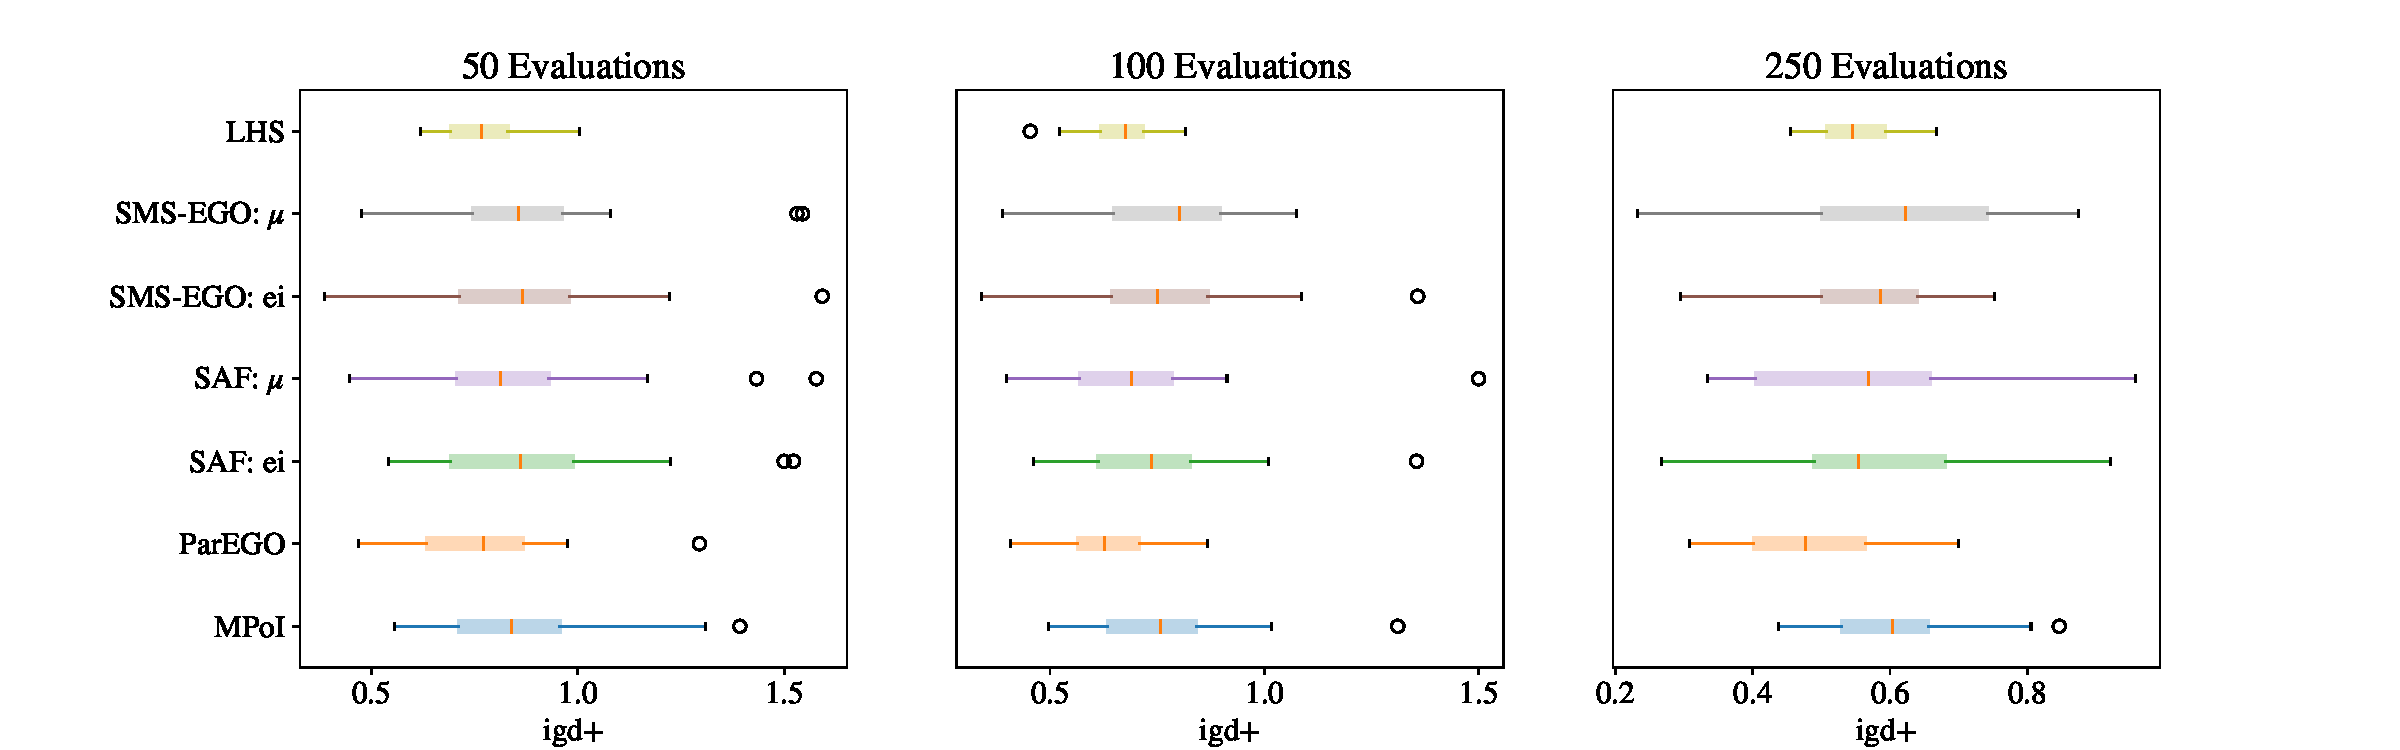
\includegraphics[width=0.8\linewidth]{figures/wfg2_4obj_10dim_igd_boxplot.pdf}
    % \caption{Caption}
\end{subfigure}
    \caption{Box plots showing Dominated Hypervolume and IGD+ over 31 repeats at three stages of the optimisation process.}
\end{figure*}
\clearpage

\begin{figure*}
WFG3\_2M\_6d


\begin{subfigure}[hbt!]{\linewidth}

    \centering
    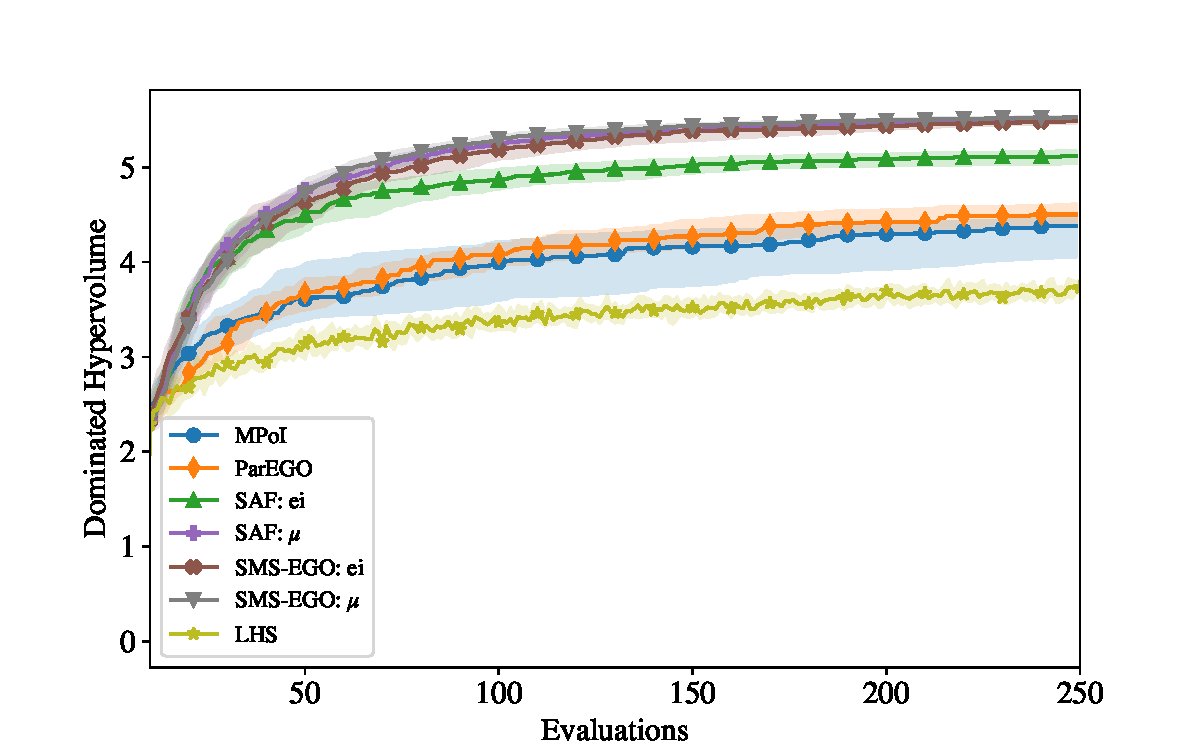
\includegraphics[width=0.7\linewidth]{figures/wfg3_2obj_6dim_hv_plot.pdf}
    % \caption{Caption}
\end{subfigure}
\begin{subfigure}[h]{\linewidth}
    \centering
    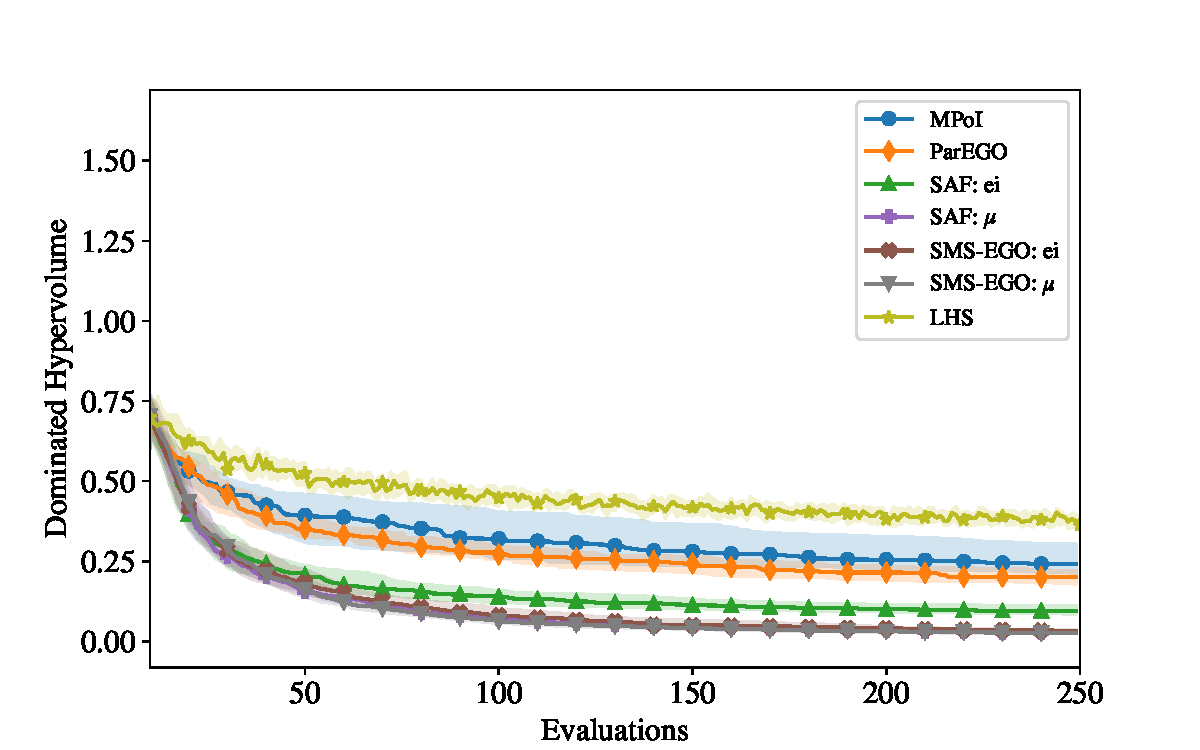
\includegraphics[width=0.7\linewidth]{figures/wfg3_2obj_6dim_igd_plot.pdf}
    % \caption{Caption}
\end{subfigure}
    \caption{Convergence plots showing median Dominated Hypervolume and IGD+ over 31 repeats. IQR shown in shaded region. Dominated hypervolume calculated as a fraction of the maximum possible.}
\vspace{\floatsep}
\begin{subfigure}[t]{\linewidth}
    \centering
    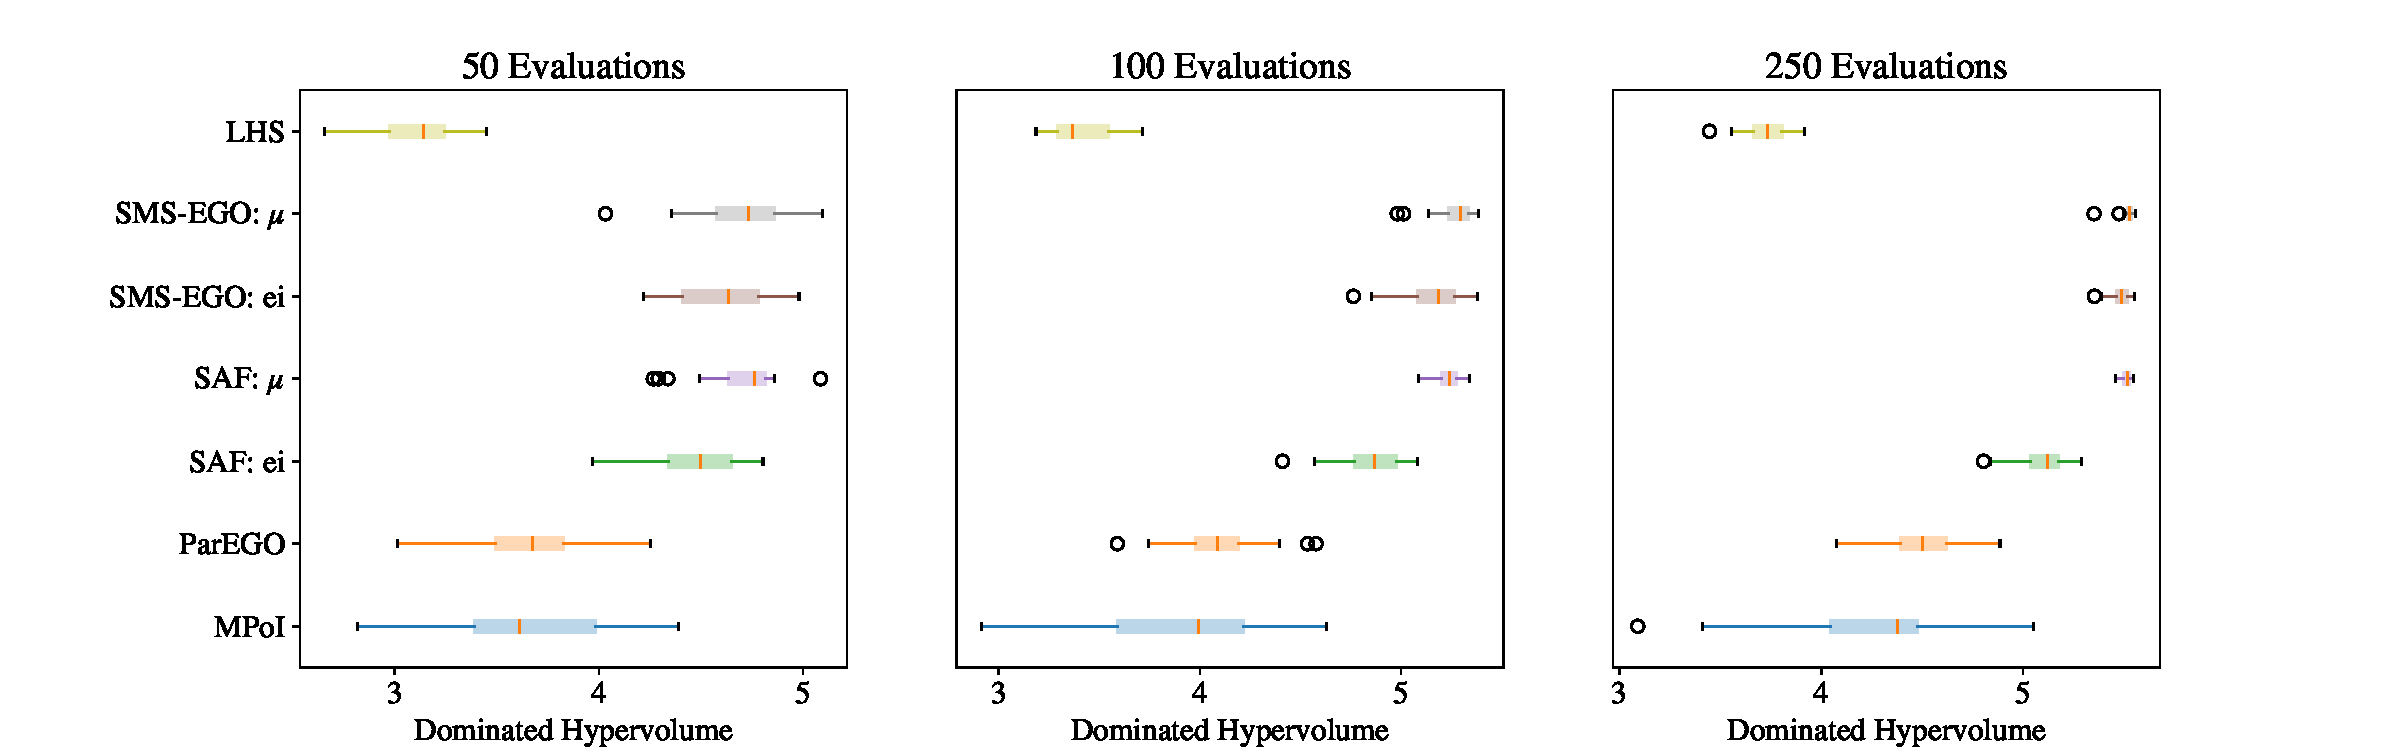
\includegraphics[width=0.8\linewidth]{figures/wfg3_2obj_6dim_hv_boxplot.pdf}
    % \caption{Caption}
\end{subfigure}
\begin{subfigure}[t]{\linewidth}
    \centering
    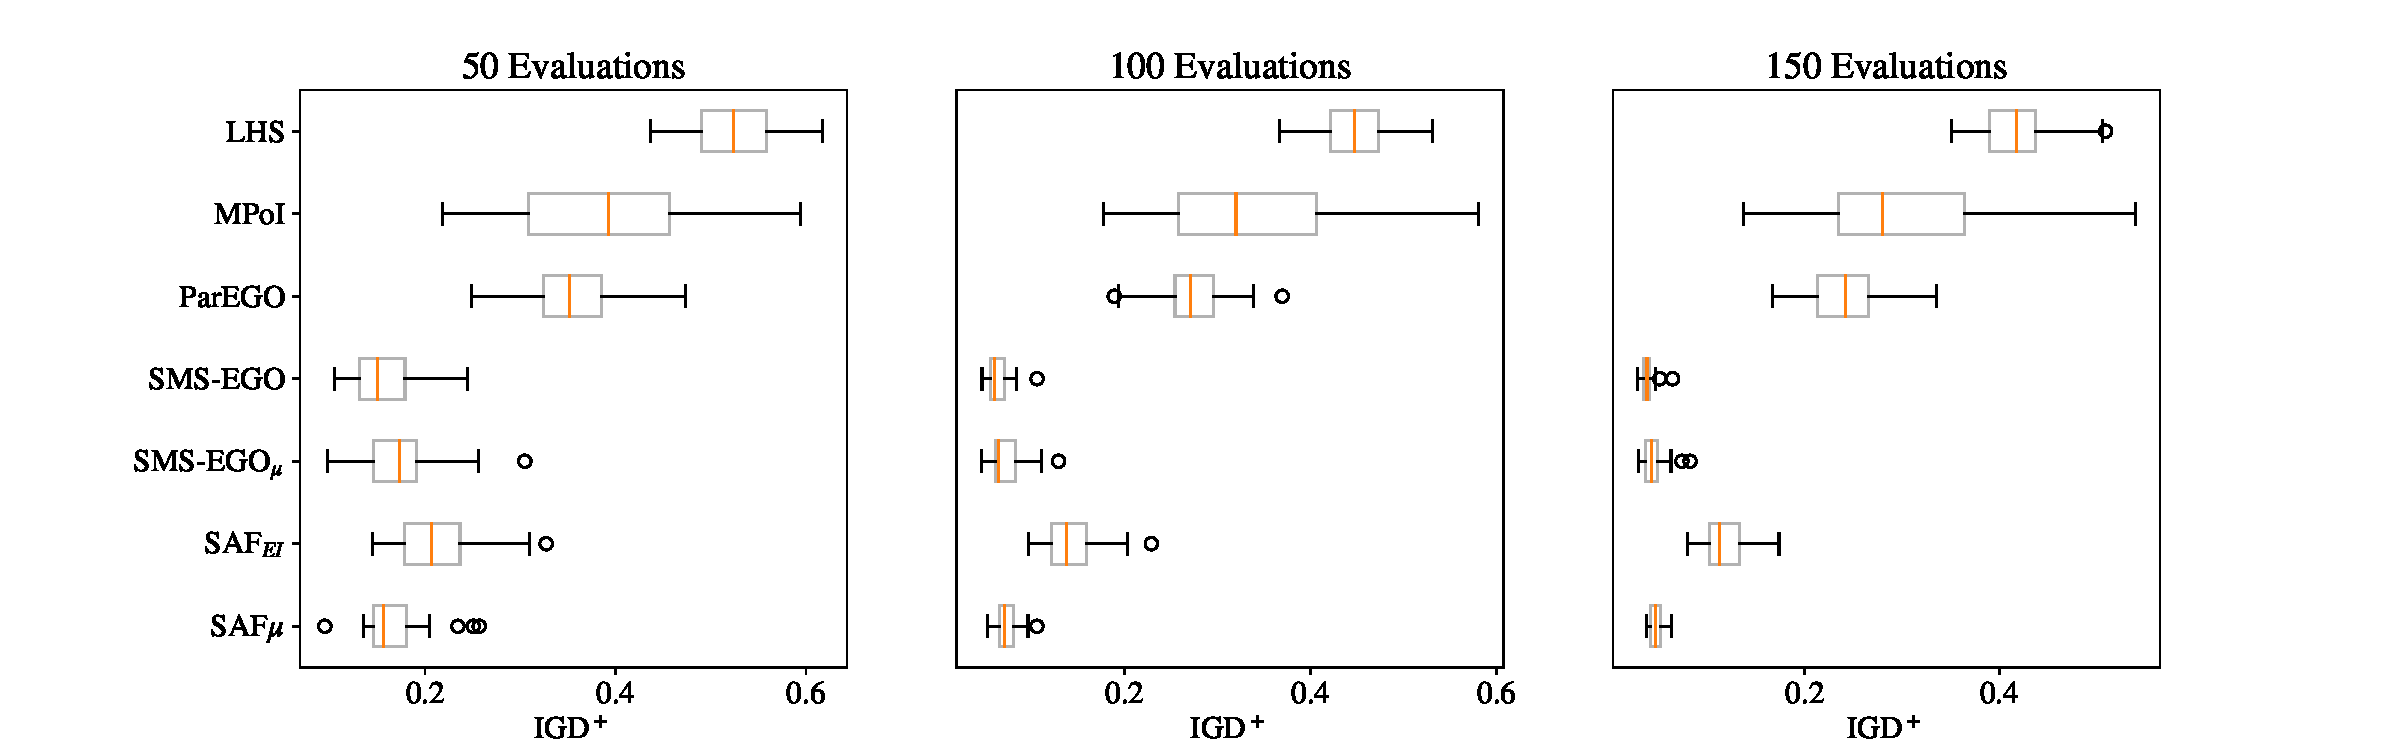
\includegraphics[width=0.8\linewidth]{figures/wfg3_2obj_6dim_igd_boxplot.pdf}
    % \caption{Caption}
\end{subfigure}
    \caption{Box plots showing Dominated Hypervolume and IGD+ over 31 repeats at three stages of the optimisation process.}
\end{figure*}
\clearpage

\begin{figure*}
WFG3\_3M\_10d


\begin{subfigure}[hbt!]{\linewidth}

    \centering
    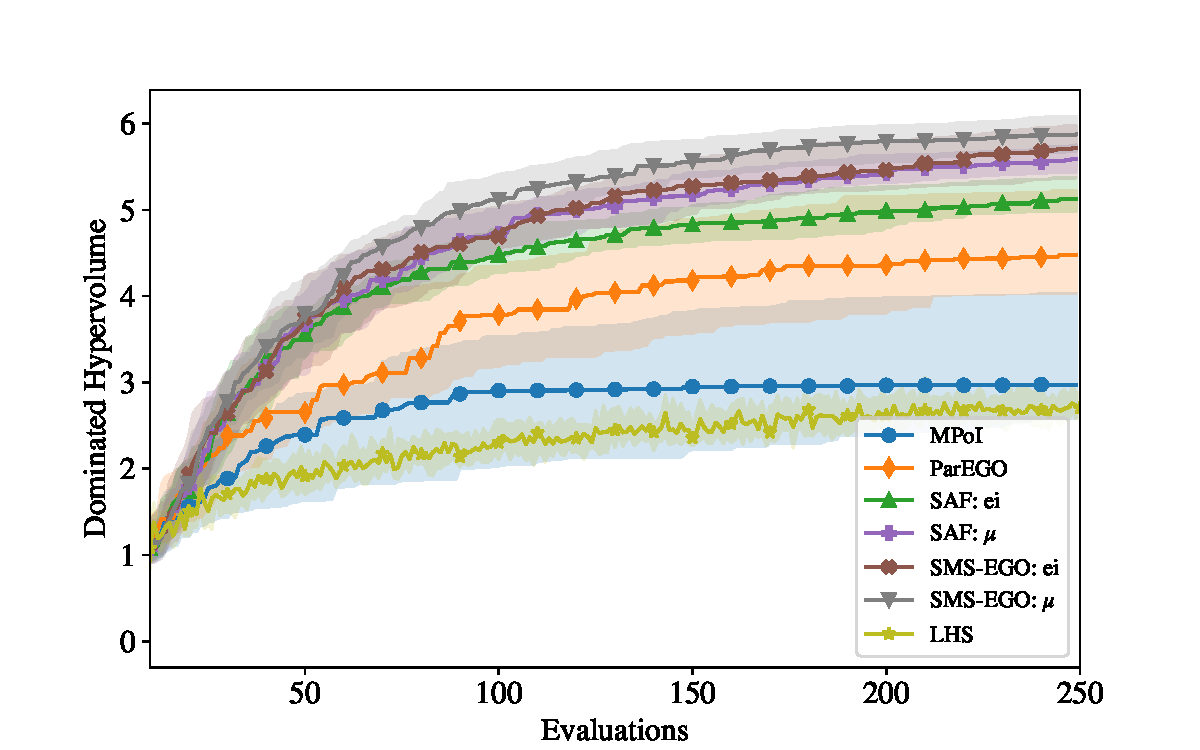
\includegraphics[width=0.7\linewidth]{figures/wfg3_3obj_10dim_hv_plot.pdf}
    % \caption{Caption}
\end{subfigure}
\begin{subfigure}[h]{\linewidth}
    \centering
    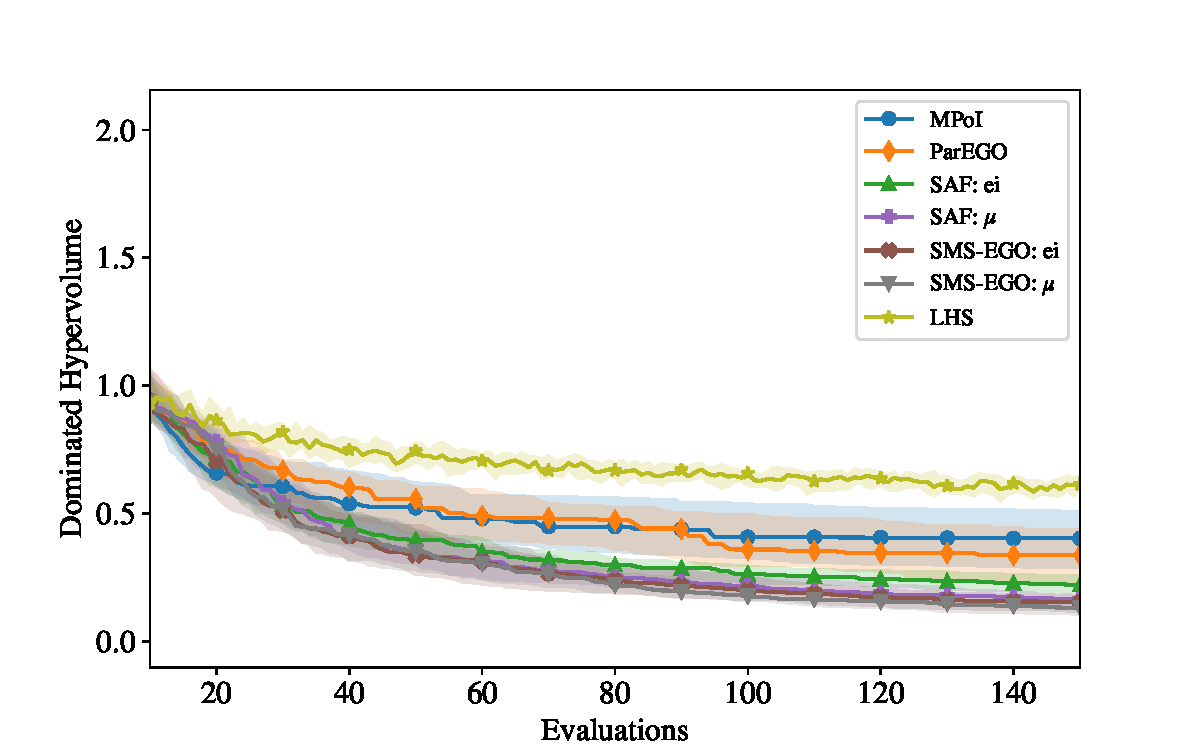
\includegraphics[width=0.7\linewidth]{figures/wfg3_3obj_10dim_igd_plot.pdf}
    % \caption{Caption}
\end{subfigure}
    \caption{Convergence plots showing median Dominated Hypervolume and IGD+ over 31 repeats. IQR shown in shaded region. Dominated hypervolume calculated as a fraction of the maximum possible.}
\vspace{\floatsep}
\begin{subfigure}[t]{\linewidth}
    \centering
    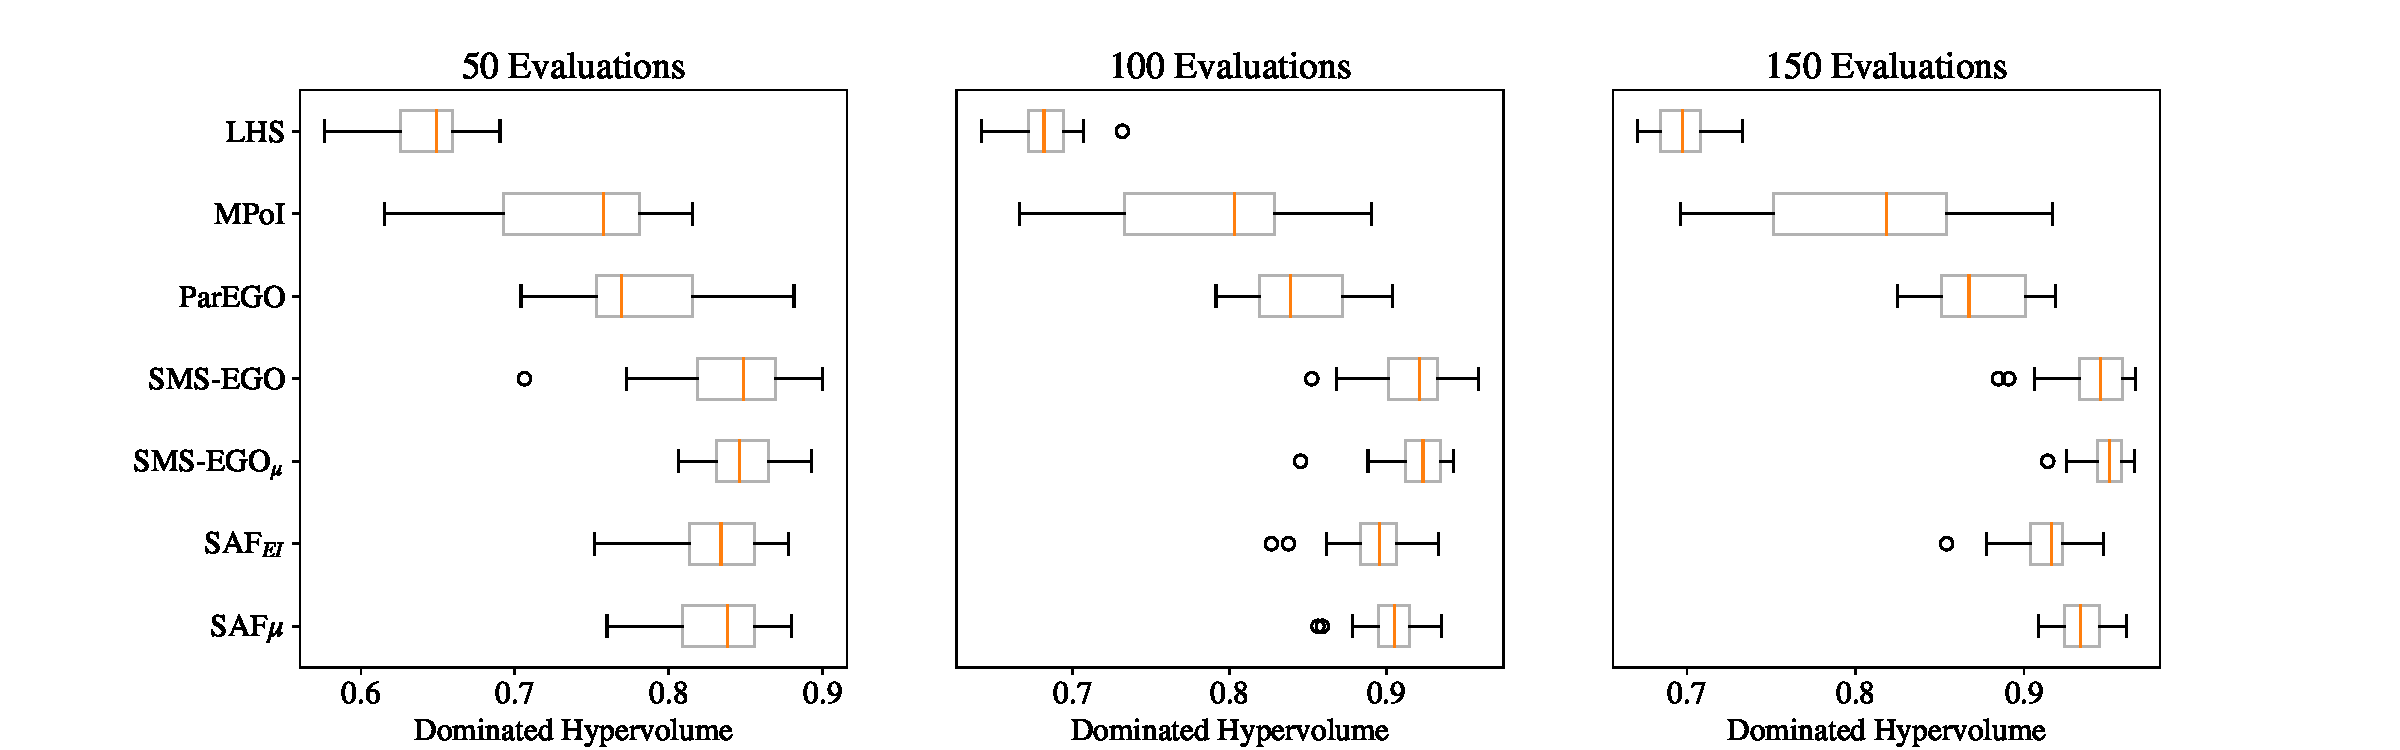
\includegraphics[width=0.8\linewidth]{figures/wfg3_3obj_10dim_hv_boxplot.pdf}
    % \caption{Caption}
\end{subfigure}
\begin{subfigure}[t]{\linewidth}
    \centering
    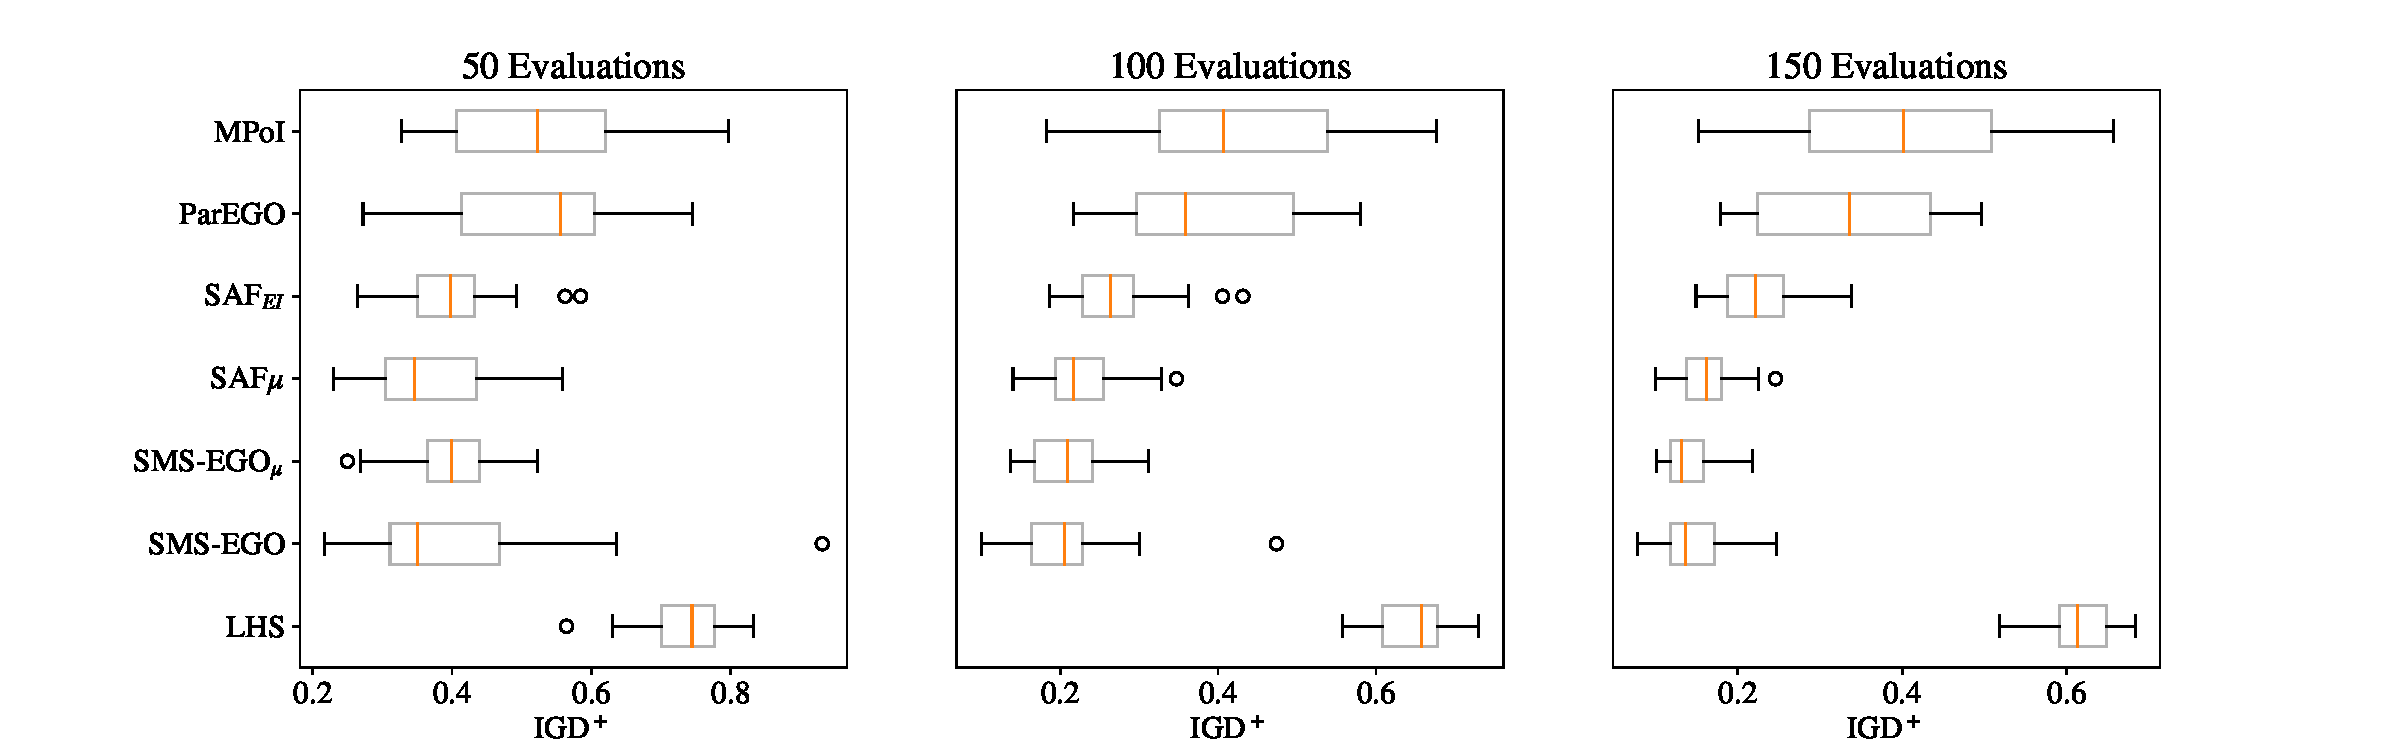
\includegraphics[width=0.8\linewidth]{figures/wfg3_3obj_10dim_igd_boxplot.pdf}
    % \caption{Caption}
\end{subfigure}
    \caption{Box plots showing Dominated Hypervolume and IGD+ over 31 repeats at three stages of the optimisation process.}
\end{figure*}
\clearpage

\begin{figure*}
WFG3\_4M\_10d


\begin{subfigure}[hbt!]{\linewidth}

    \centering
    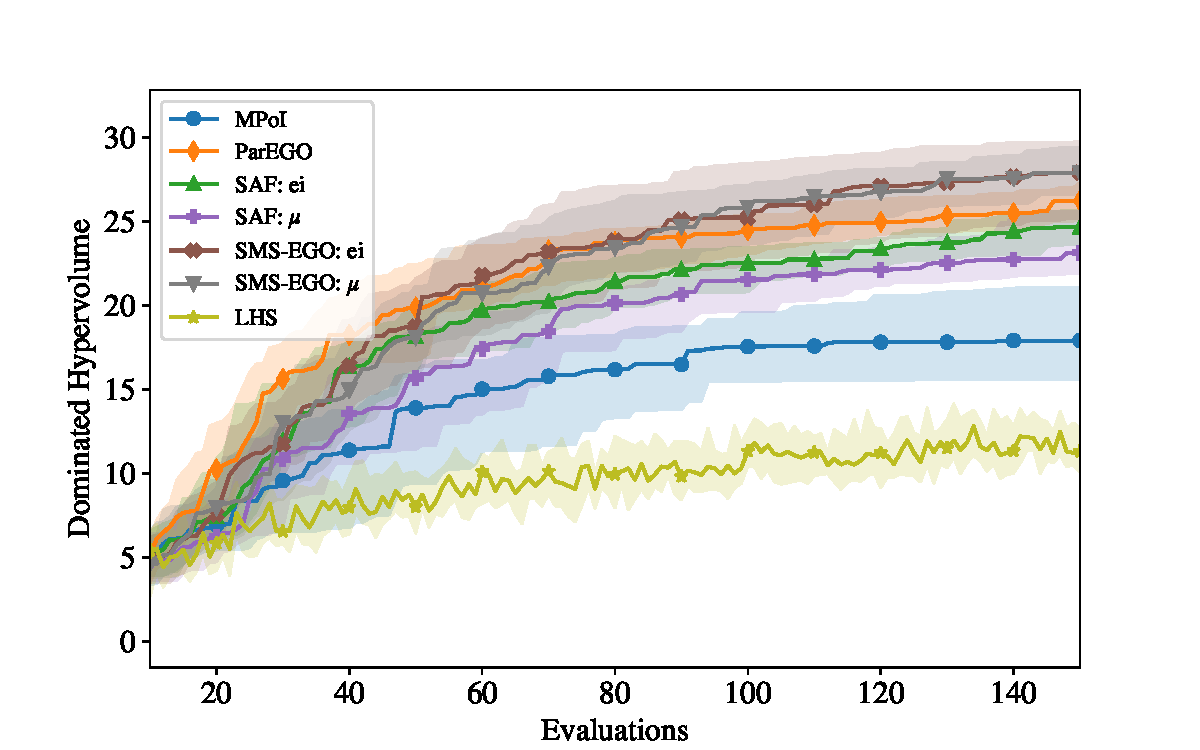
\includegraphics[width=0.7\linewidth]{figures/wfg3_4obj_10dim_hv_plot.pdf}
    % \caption{Caption}
\end{subfigure}
\begin{subfigure}[h]{\linewidth}
    \centering
    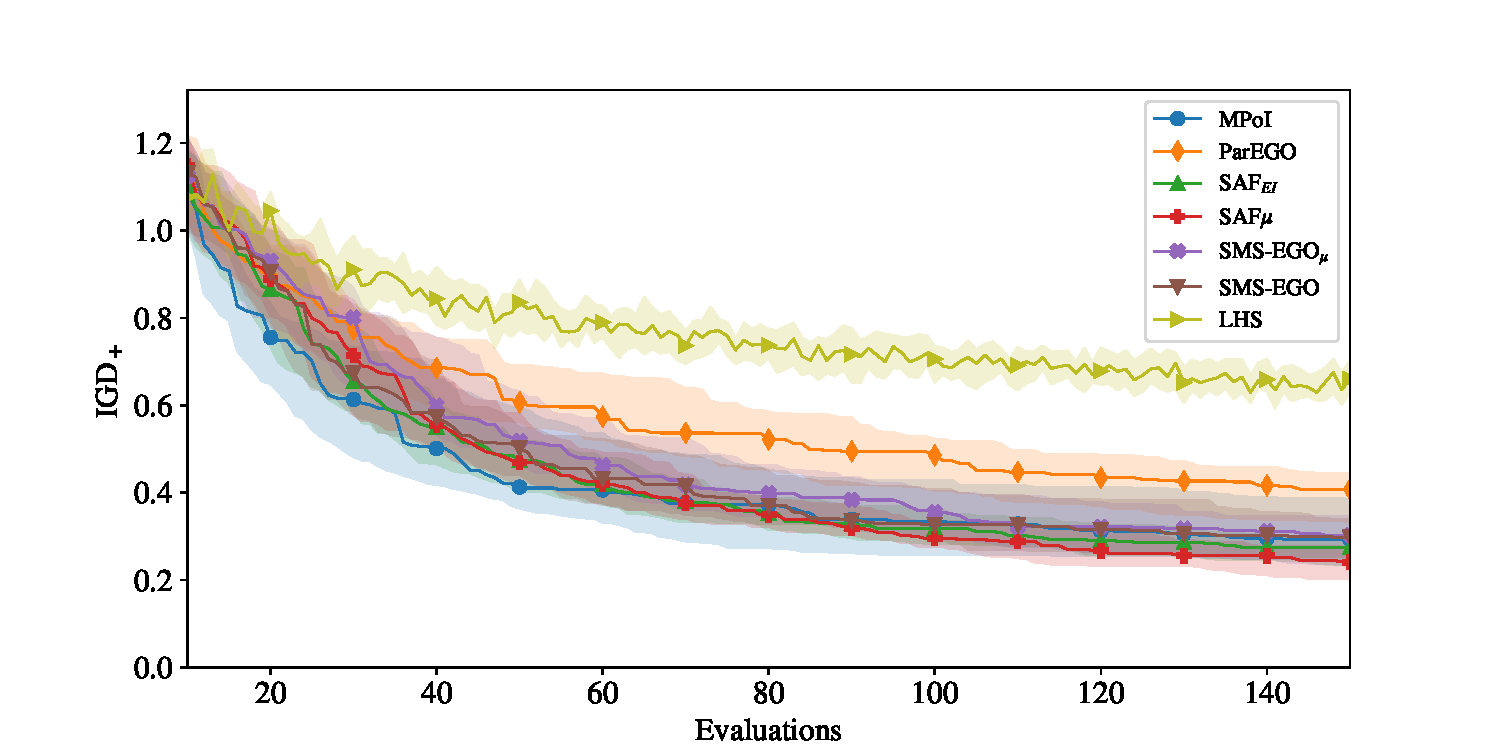
\includegraphics[width=0.7\linewidth]{figures/wfg3_4obj_10dim_igd_plot.pdf}
    % \caption{Caption}
\end{subfigure}
    \caption{Convergence plots showing median Dominated Hypervolume and IGD+ over 31 repeats. IQR shown in shaded region. Dominated hypervolume calculated as a fraction of the maximum possible.}
\vspace{\floatsep}
\begin{subfigure}[t]{\linewidth}
    \centering
    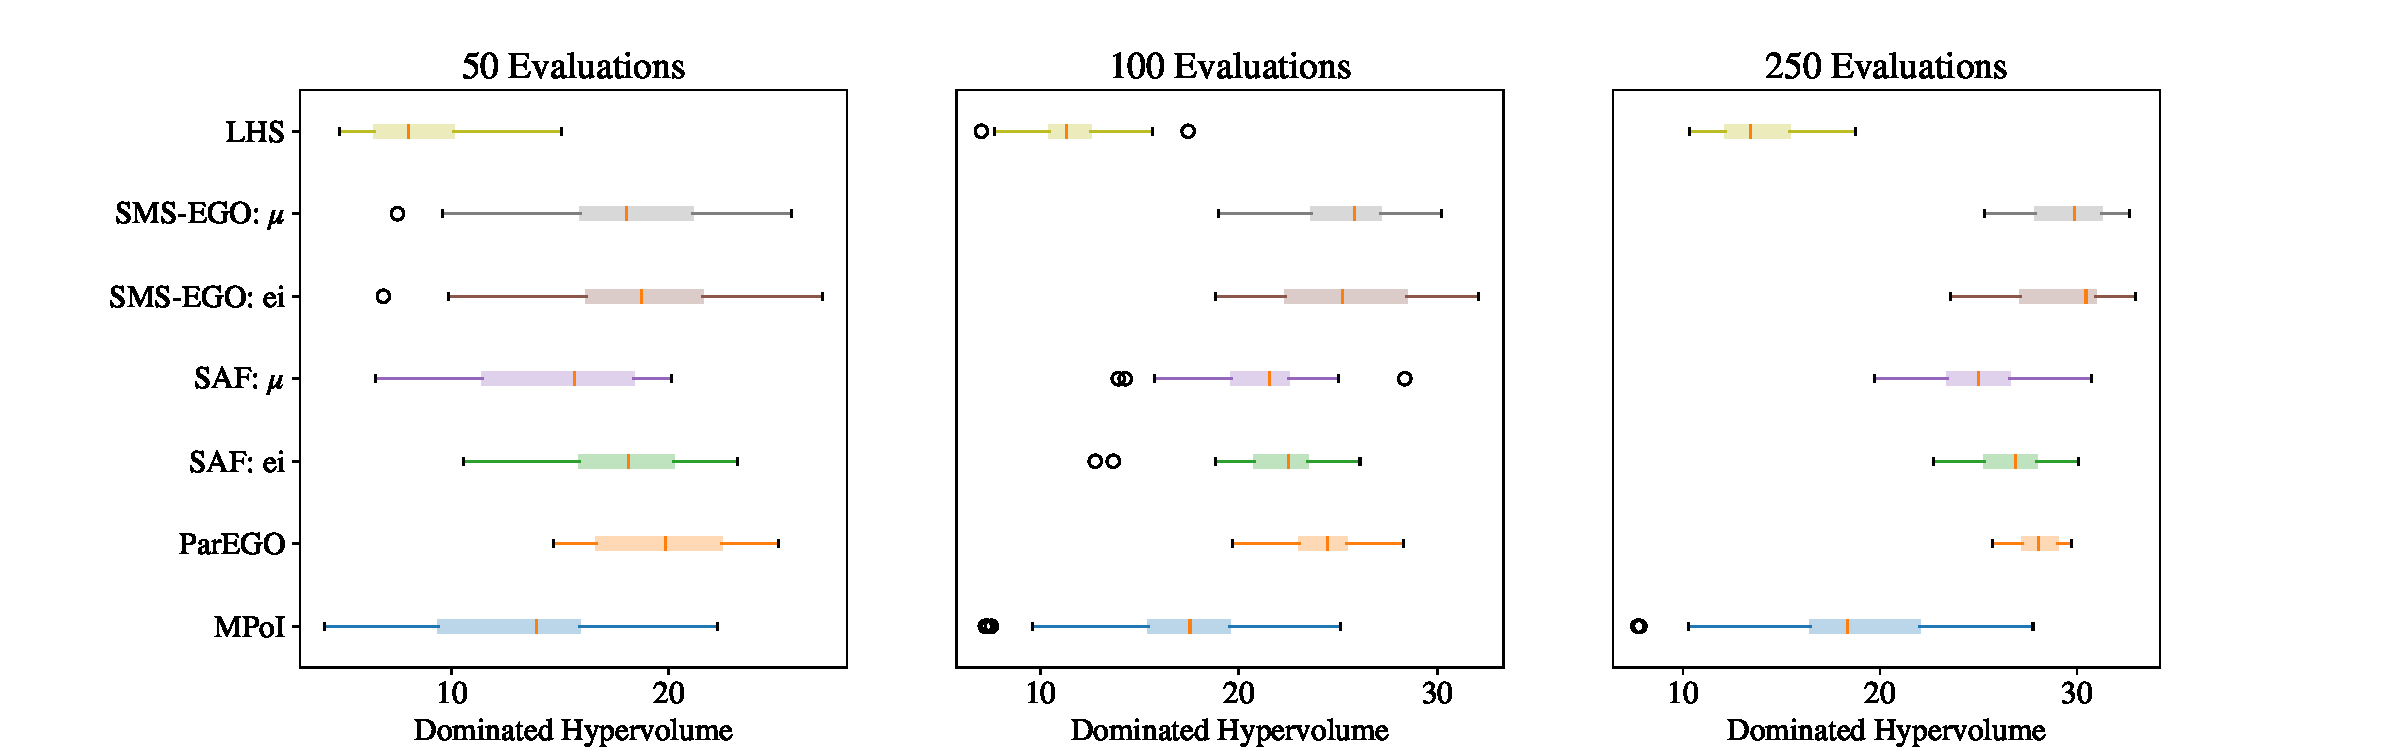
\includegraphics[width=0.8\linewidth]{figures/wfg3_4obj_10dim_hv_boxplot.pdf}
    % \caption{Caption}
\end{subfigure}
\begin{subfigure}[t]{\linewidth}
    \centering
    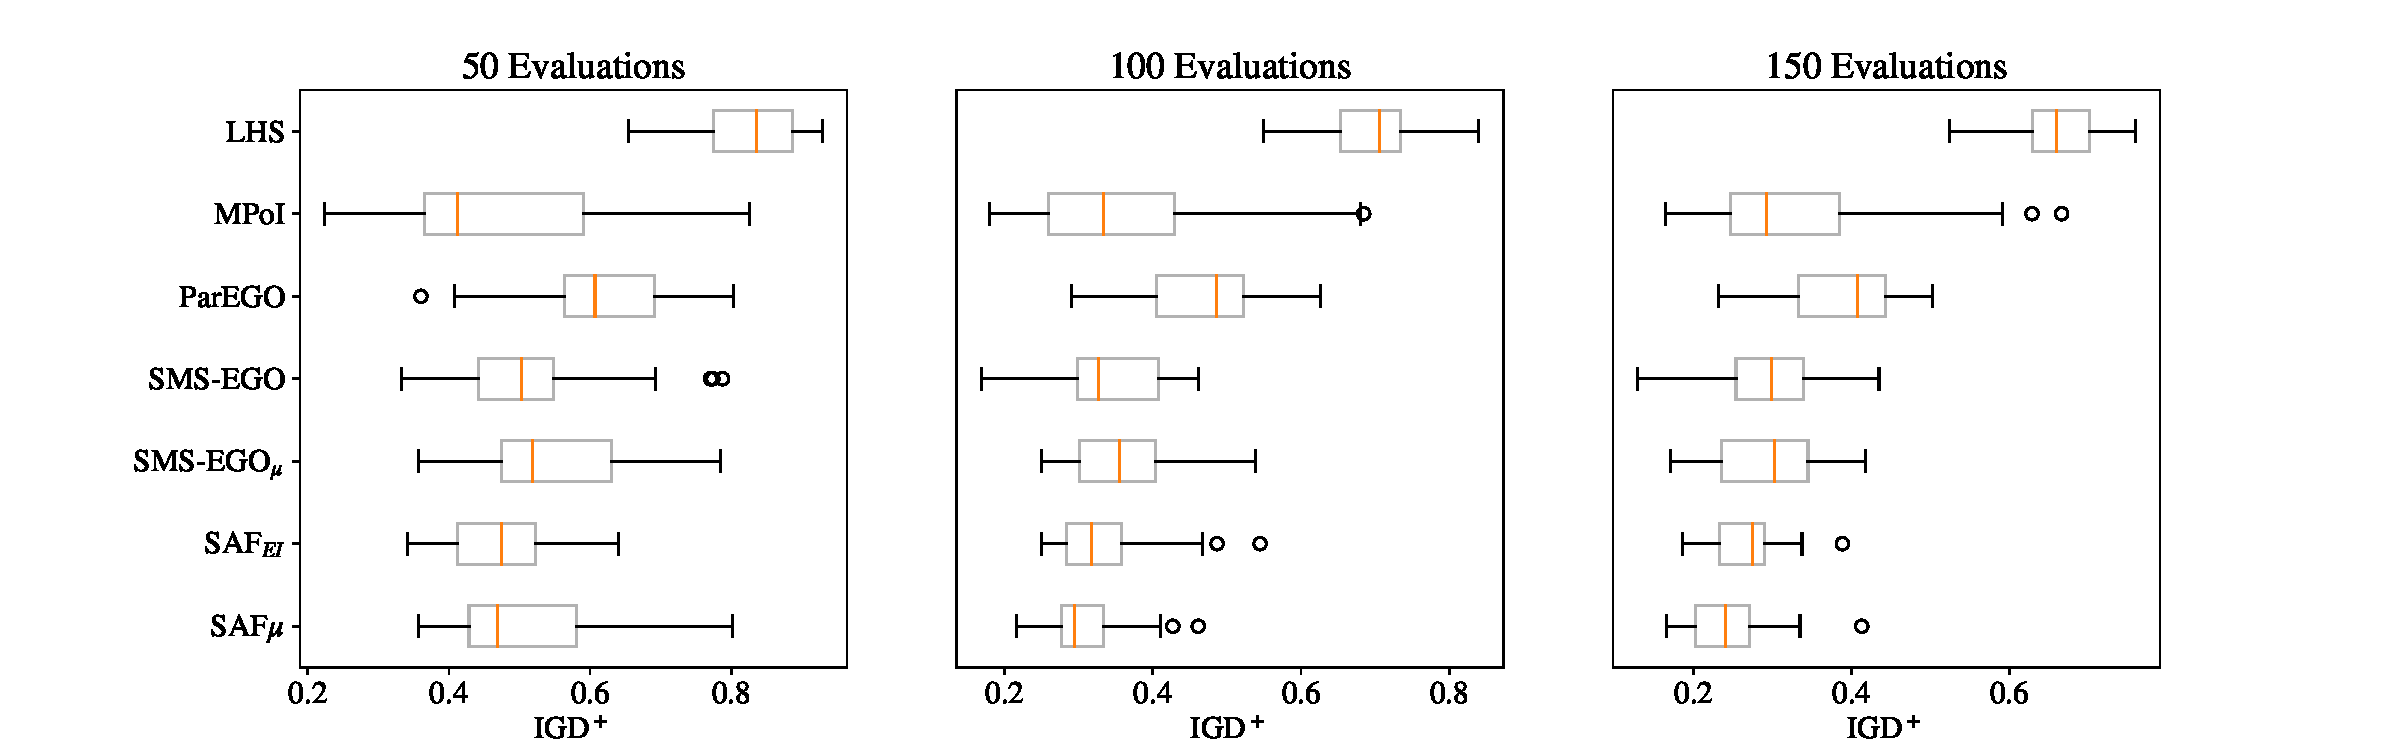
\includegraphics[width=0.8\linewidth]{figures/wfg3_4obj_10dim_igd_boxplot.pdf}
    % \caption{Caption}
\end{subfigure}
    \caption{Box plots showing Dominated Hypervolume and IGD+ over 31 repeats at three stages of the optimisation process.}
\end{figure*}
\clearpage

\begin{figure*}
WFG4\_2M\_6d


\begin{subfigure}[hbt!]{\linewidth}

    \centering
    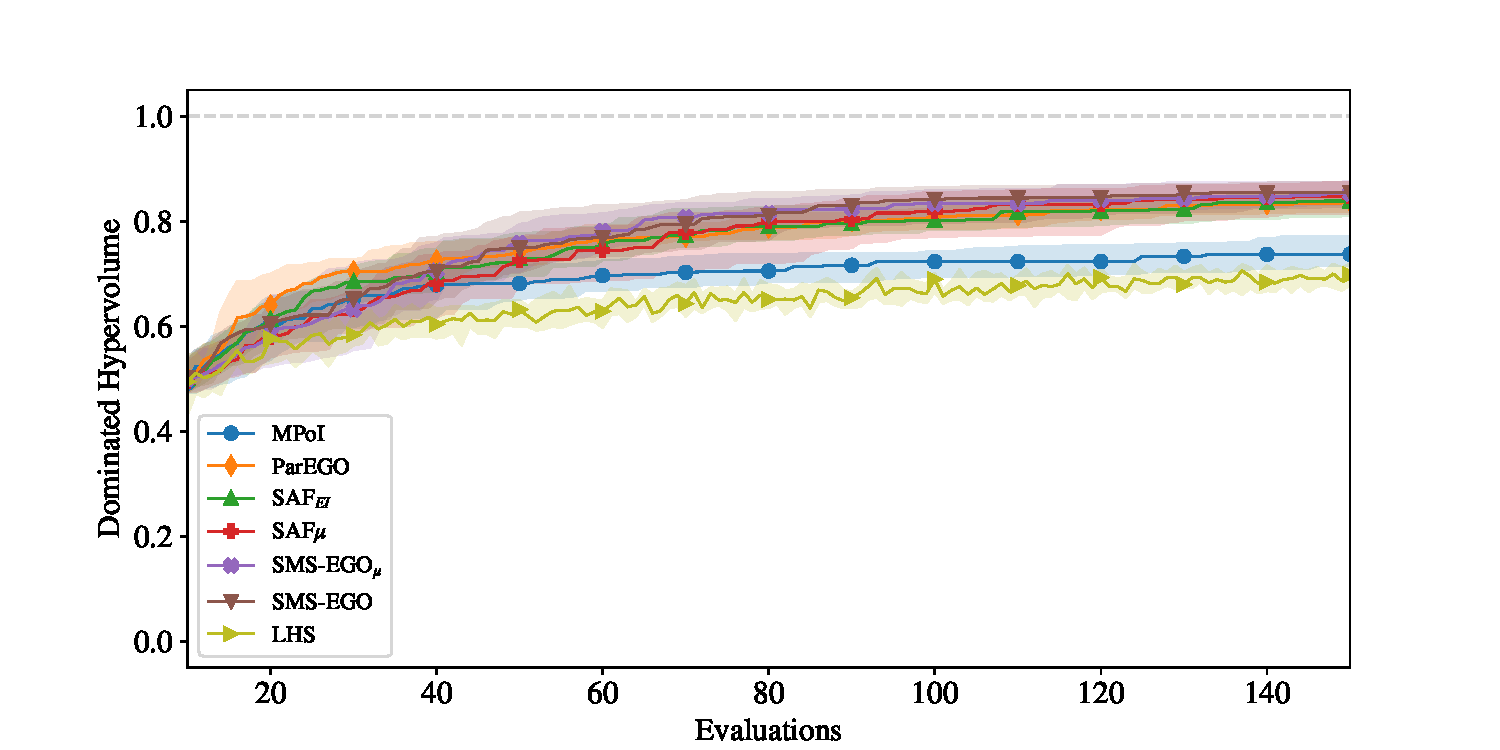
\includegraphics[width=0.7\linewidth]{figures/wfg4_2obj_6dim_hv_plot.pdf}
    % \caption{Caption}
\end{subfigure}
\begin{subfigure}[h]{\linewidth}
    \centering
    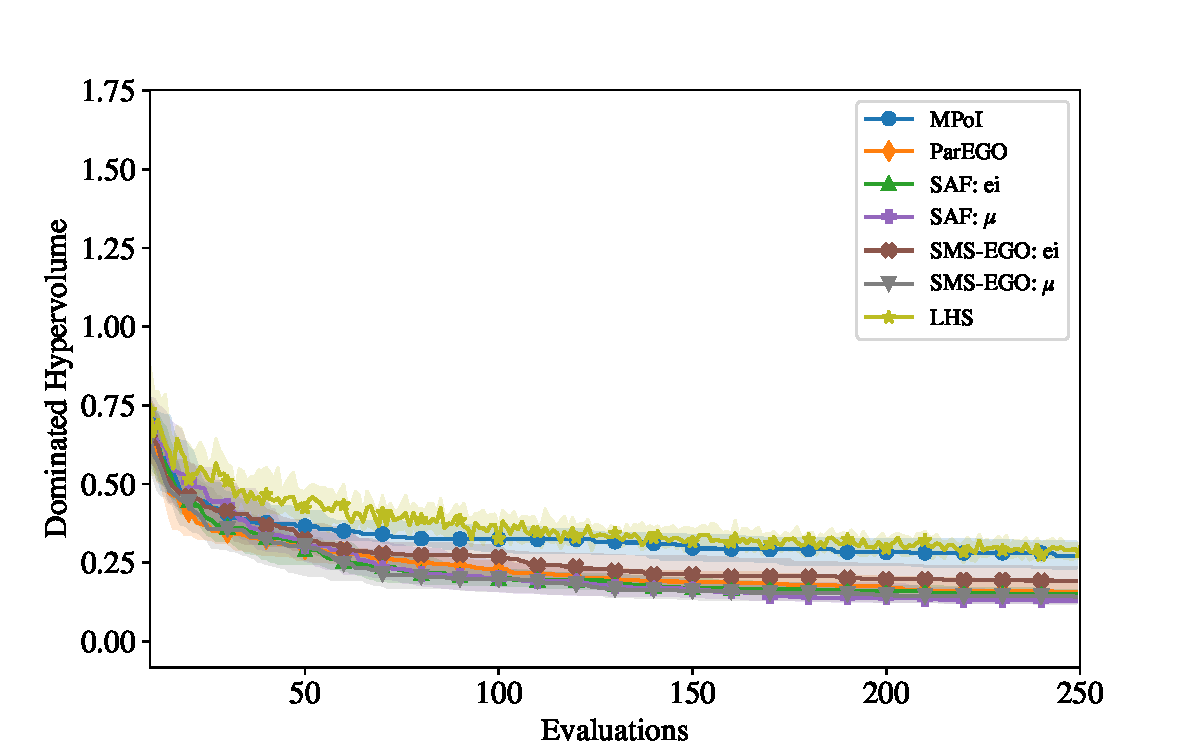
\includegraphics[width=0.7\linewidth]{figures/wfg4_2obj_6dim_igd_plot.pdf}
    % \caption{Caption}
\end{subfigure}
    \caption{Convergence plots showing median Dominated Hypervolume and IGD+ over 31 repeats. IQR shown in shaded region. Dominated hypervolume calculated as a fraction of the maximum possible.}
\vspace{\floatsep}
\begin{subfigure}[t]{\linewidth}
    \centering
    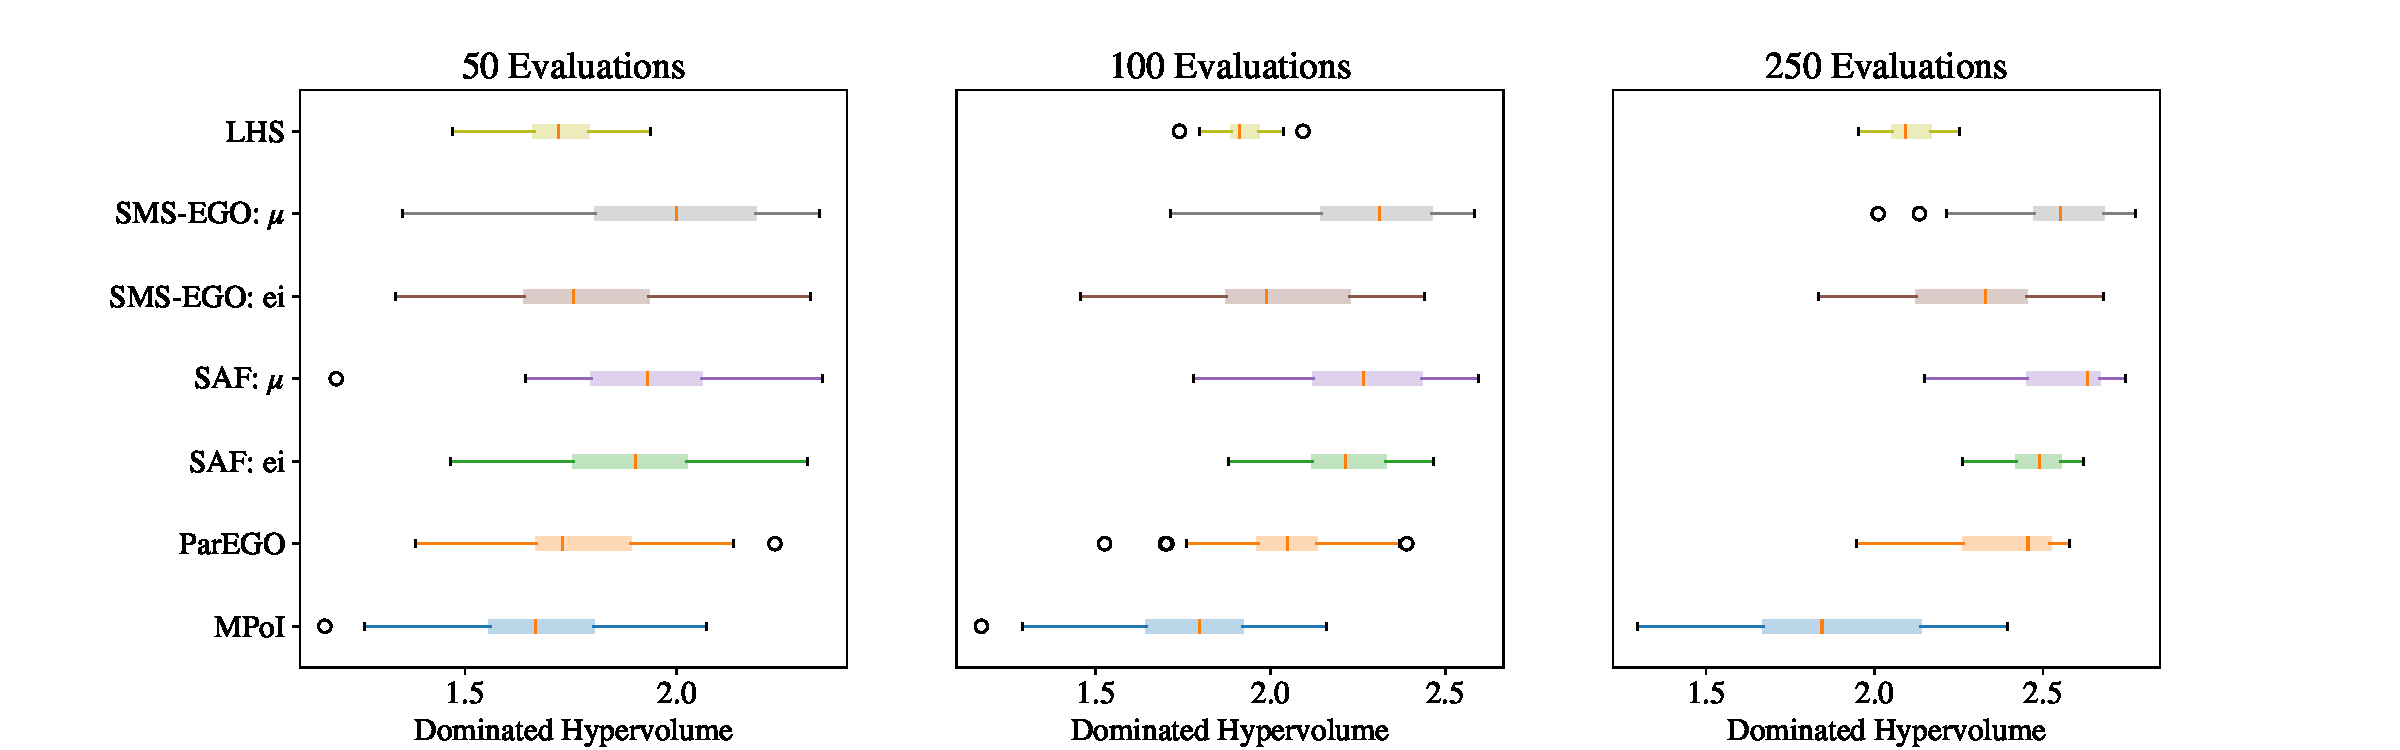
\includegraphics[width=0.8\linewidth]{figures/wfg4_2obj_6dim_hv_boxplot.pdf}
    % \caption{Caption}
\end{subfigure}
\begin{subfigure}[t]{\linewidth}
    \centering
    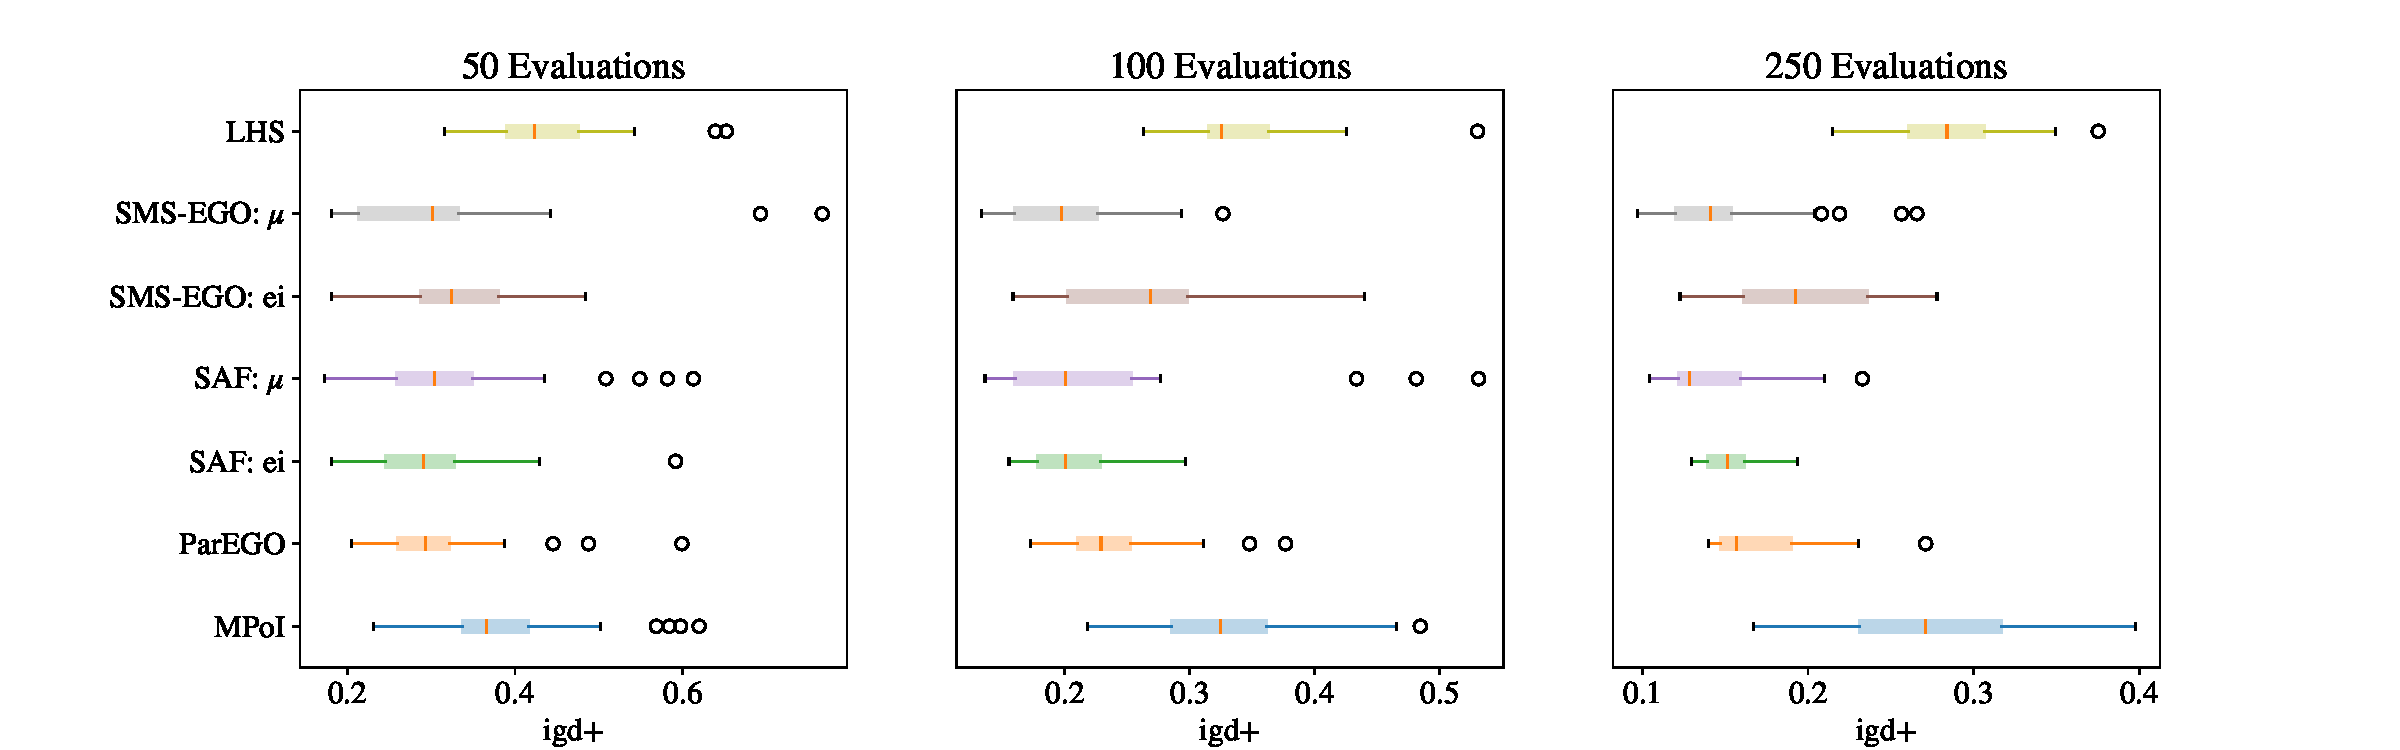
\includegraphics[width=0.8\linewidth]{figures/wfg4_2obj_6dim_igd_boxplot.pdf}
    % \caption{Caption}
\end{subfigure}
    \caption{Box plots showing Dominated Hypervolume and IGD+ over 31 repeats at three stages of the optimisation process.}
\end{figure*}
\clearpage

\begin{figure*}
WFG4\_3M\_8d


\begin{subfigure}[hbt!]{\linewidth}

    \centering
    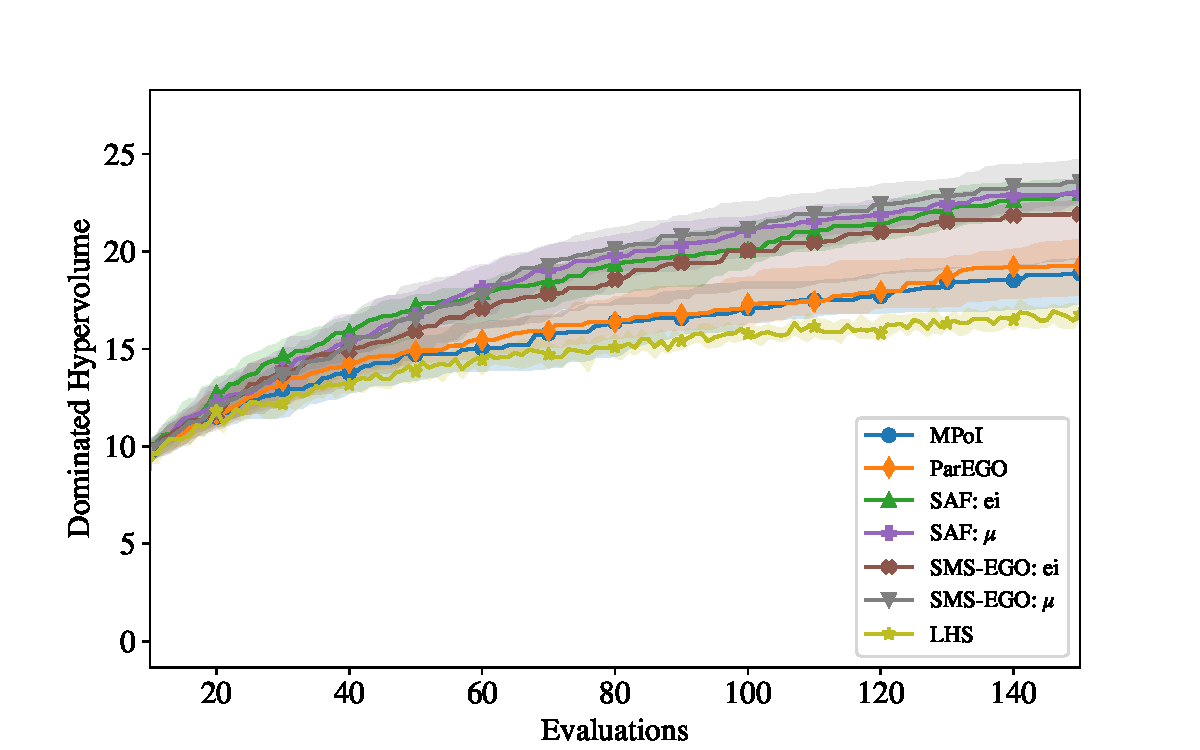
\includegraphics[width=0.7\linewidth]{figures/wfg4_3obj_8dim_hv_plot.pdf}
    % \caption{Caption}
\end{subfigure}
\begin{subfigure}[h]{\linewidth}
    \centering
    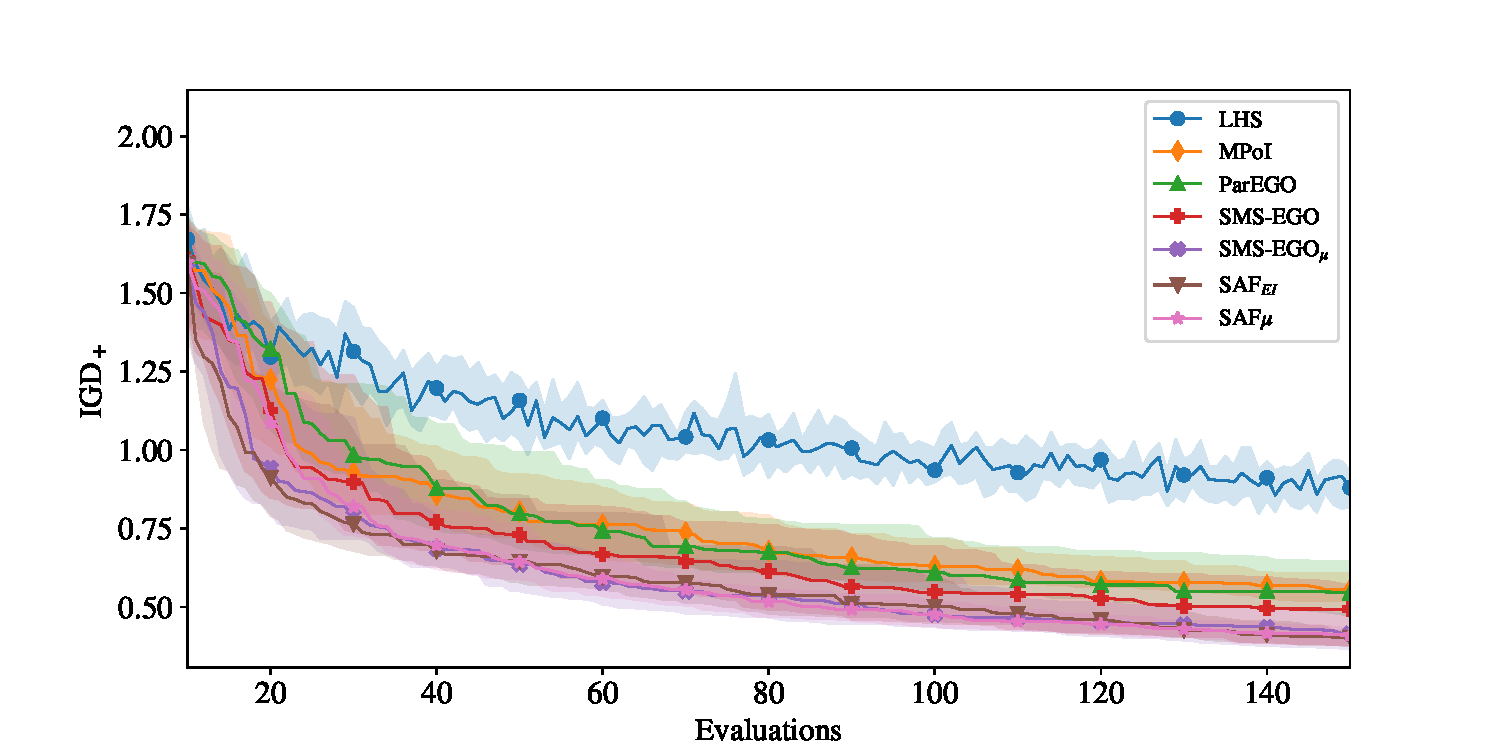
\includegraphics[width=0.7\linewidth]{figures/wfg4_3obj_8dim_igd_plot.pdf}
    % \caption{Caption}
\end{subfigure}
    \caption{Convergence plots showing median Dominated Hypervolume and IGD+ over 31 repeats. IQR shown in shaded region. Dominated hypervolume calculated as a fraction of the maximum possible.}
\vspace{\floatsep}
\begin{subfigure}[t]{\linewidth}
    \centering
    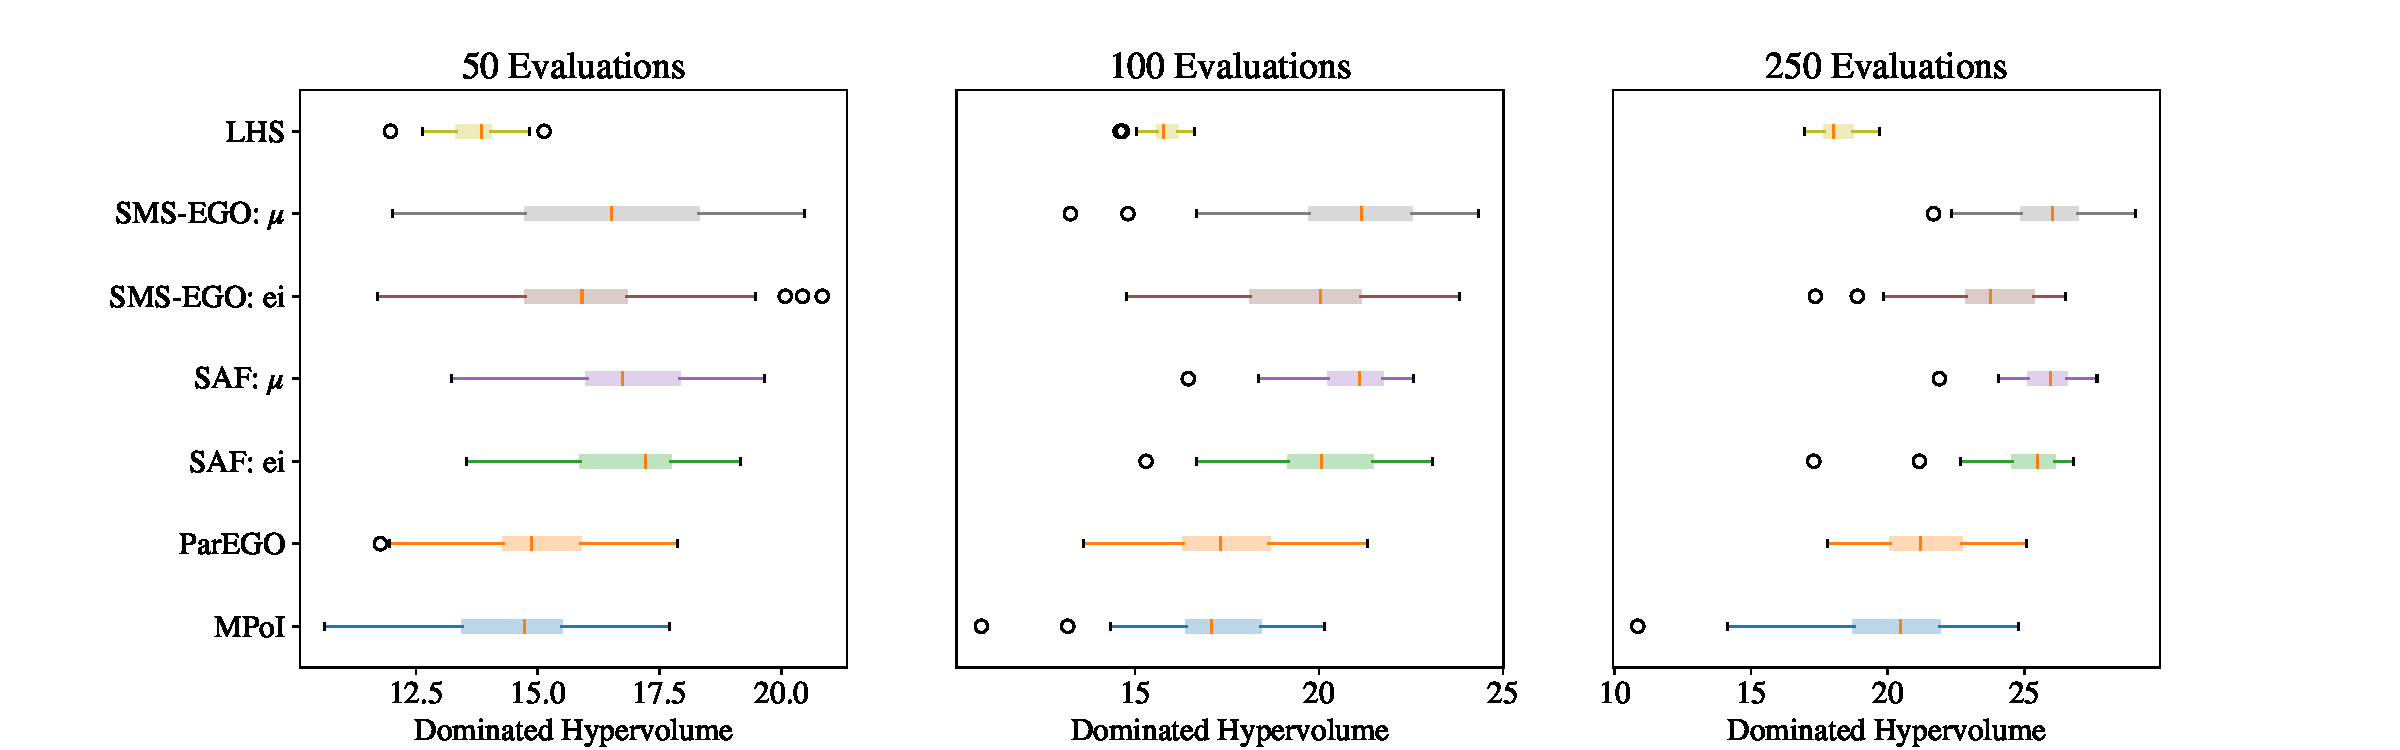
\includegraphics[width=0.8\linewidth]{figures/wfg4_3obj_8dim_hv_boxplot.pdf}
    % \caption{Caption}
\end{subfigure}
\begin{subfigure}[t]{\linewidth}
    \centering
    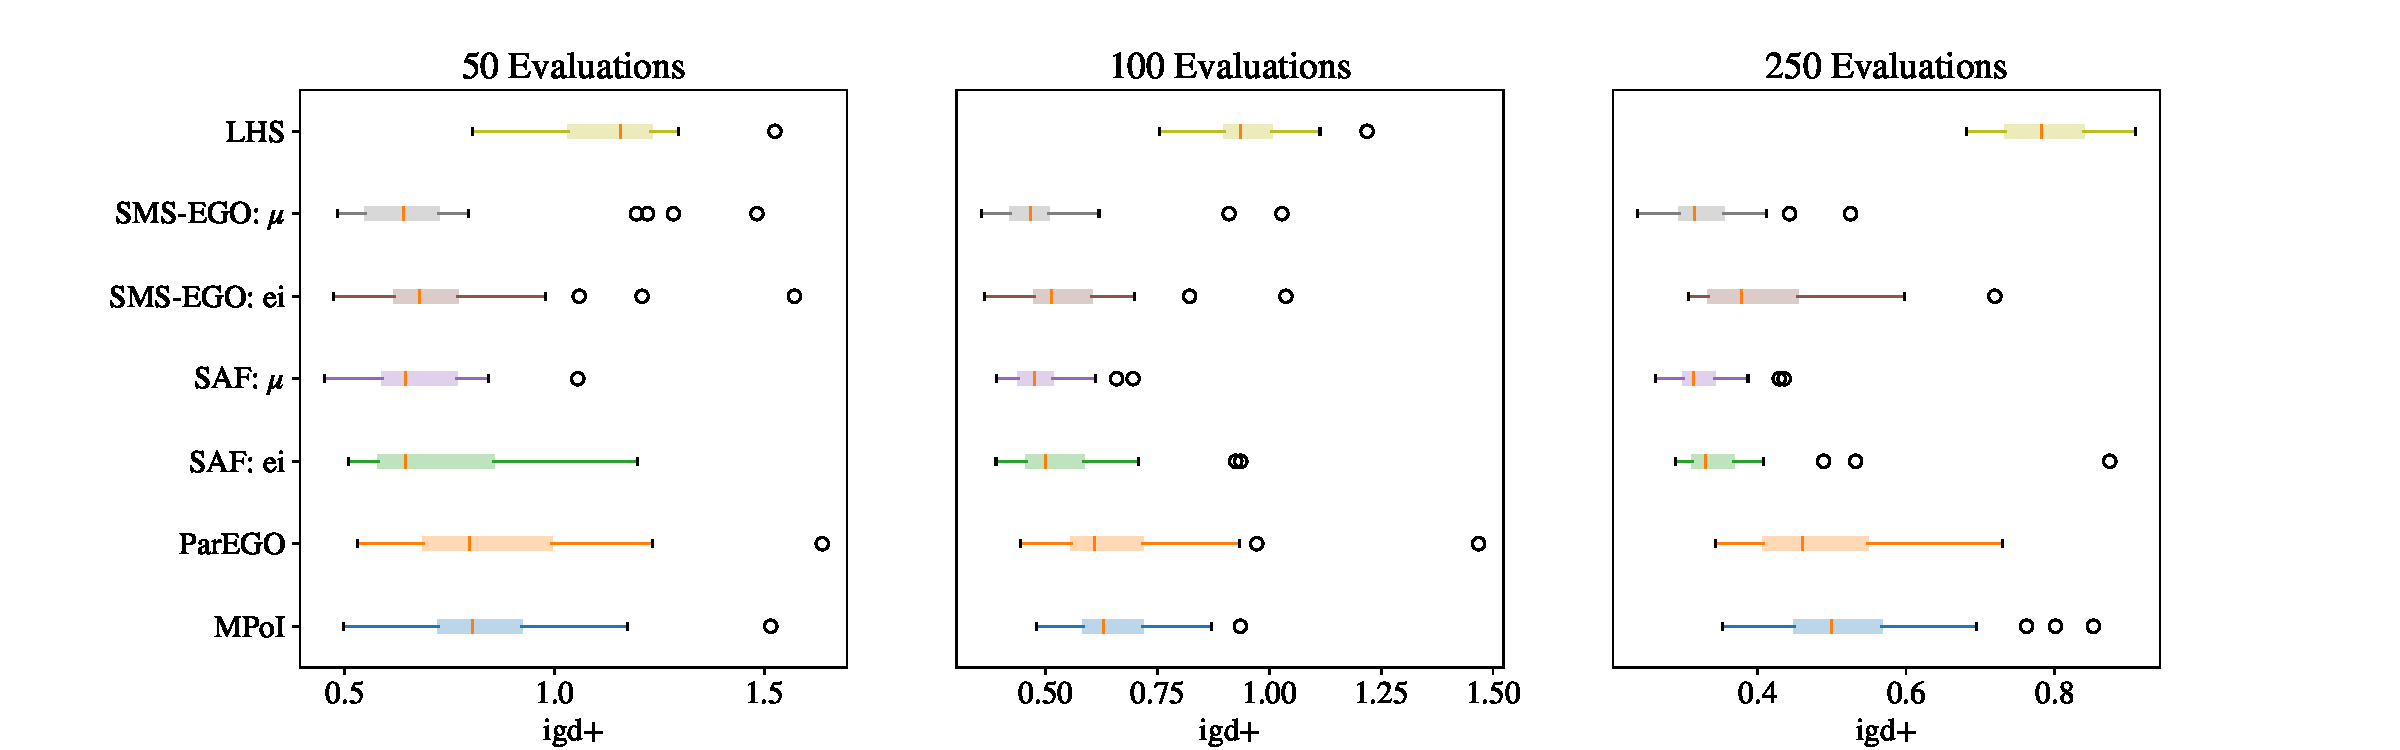
\includegraphics[width=0.8\linewidth]{figures/wfg4_3obj_8dim_igd_boxplot.pdf}
    % \caption{Caption}
\end{subfigure}
    \caption{Box plots showing Dominated Hypervolume and IGD+ over 31 repeats at three stages of the optimisation process.}
\end{figure*}
\clearpage

\begin{figure*}
WFG4\_4M\_8d


\begin{subfigure}[hbt!]{\linewidth}

    \centering
    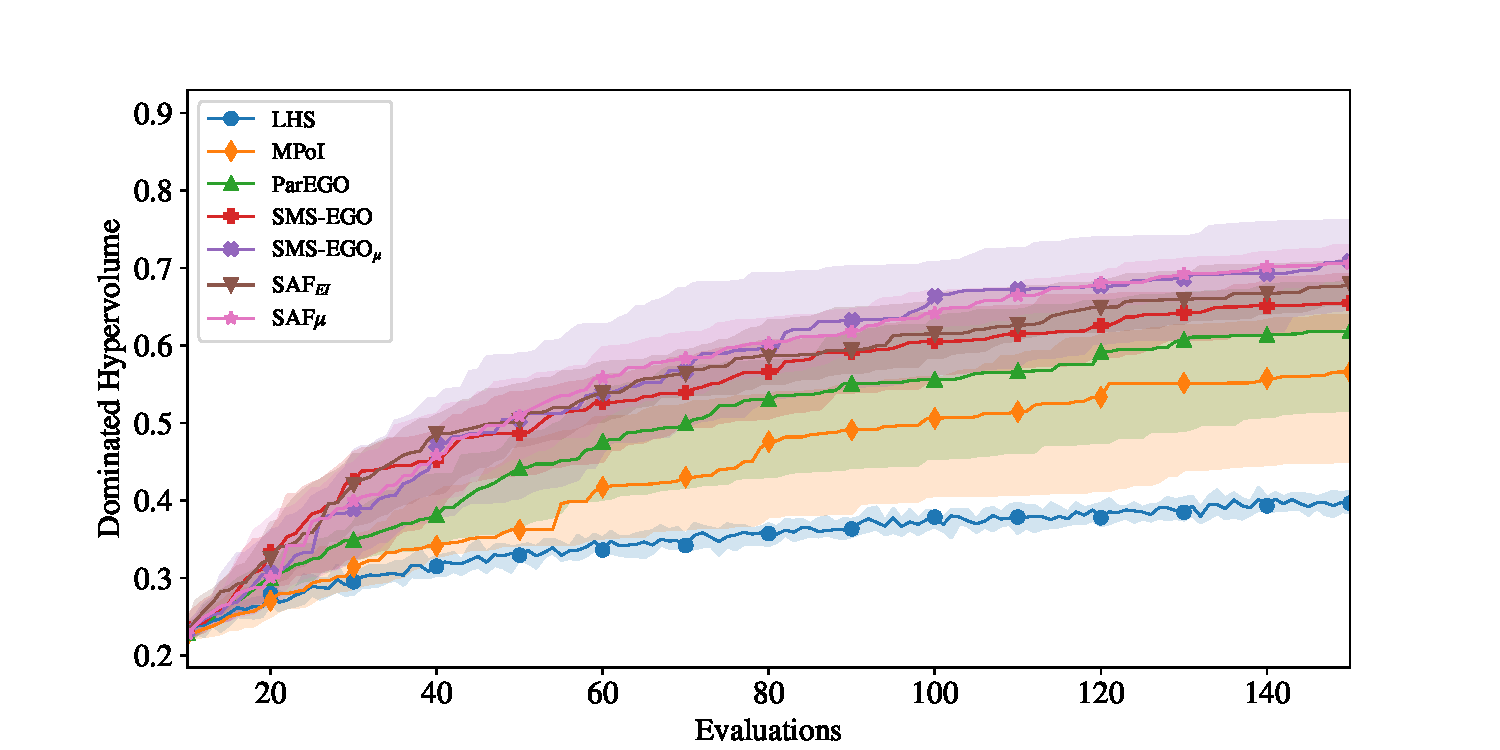
\includegraphics[width=0.7\linewidth]{figures/wfg4_4obj_8dim_hv_plot.pdf}
    % \caption{Caption}
\end{subfigure}
\begin{subfigure}[h]{\linewidth}
    \centering
    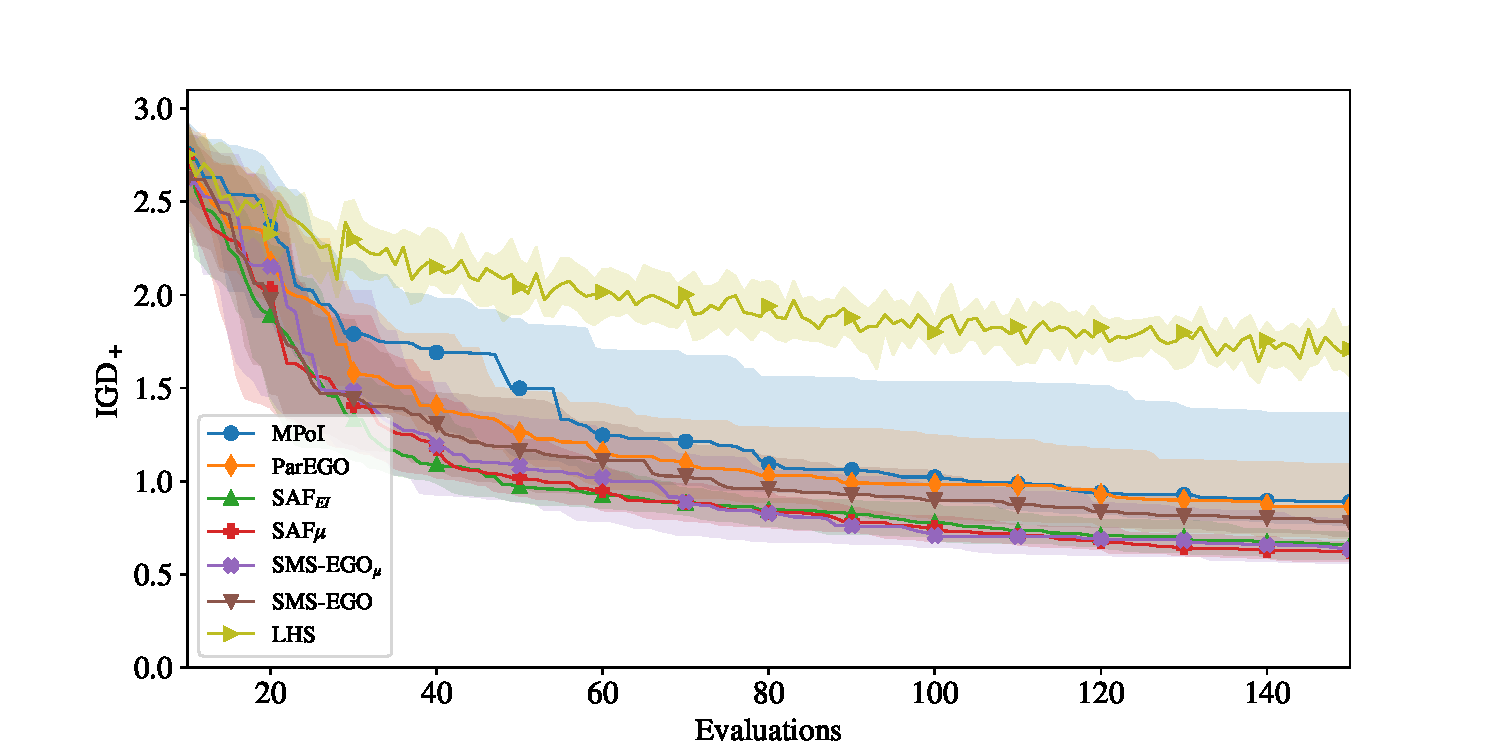
\includegraphics[width=0.7\linewidth]{figures/wfg4_4obj_8dim_igd_plot.pdf}
    % \caption{Caption}
\end{subfigure}
    \caption{Convergence plots showing median Dominated Hypervolume and IGD+ over 31 repeats. IQR shown in shaded region. Dominated hypervolume calculated as a fraction of the maximum possible.}
\vspace{\floatsep}
\begin{subfigure}[t]{\linewidth}
    \centering
    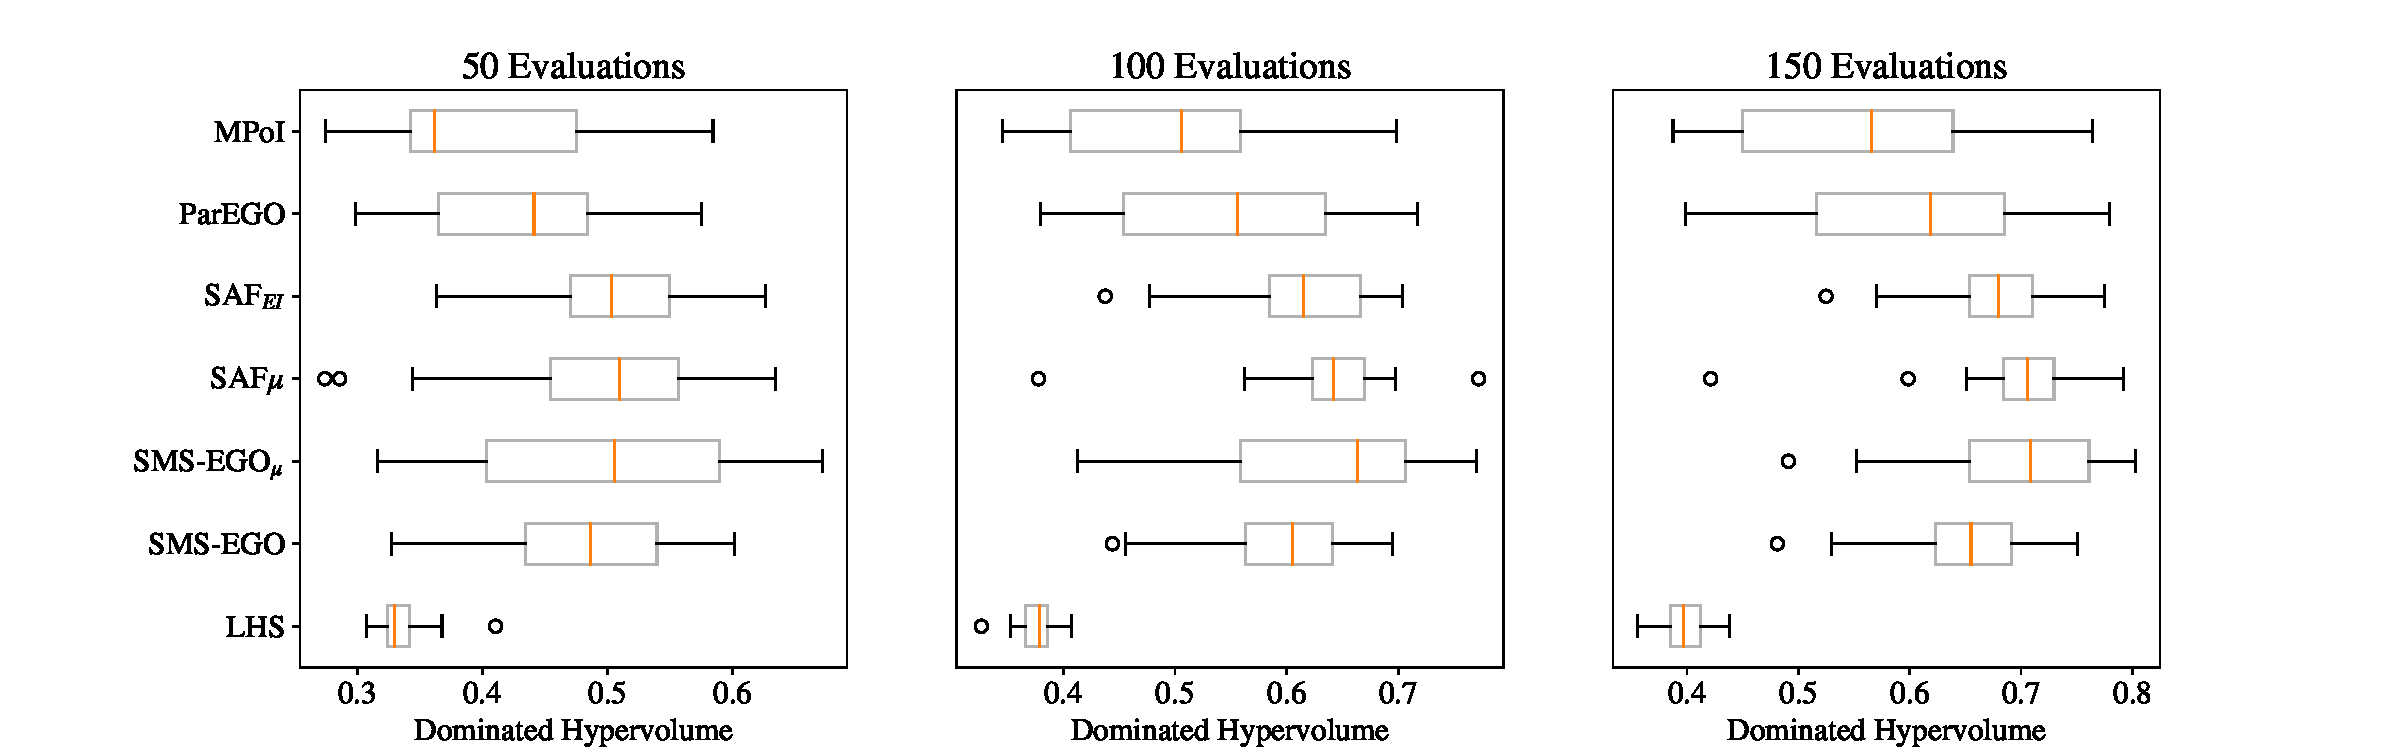
\includegraphics[width=0.8\linewidth]{figures/wfg4_4obj_8dim_hv_boxplot.pdf}
    % \caption{Caption}
\end{subfigure}
\begin{subfigure}[t]{\linewidth}
    \centering
    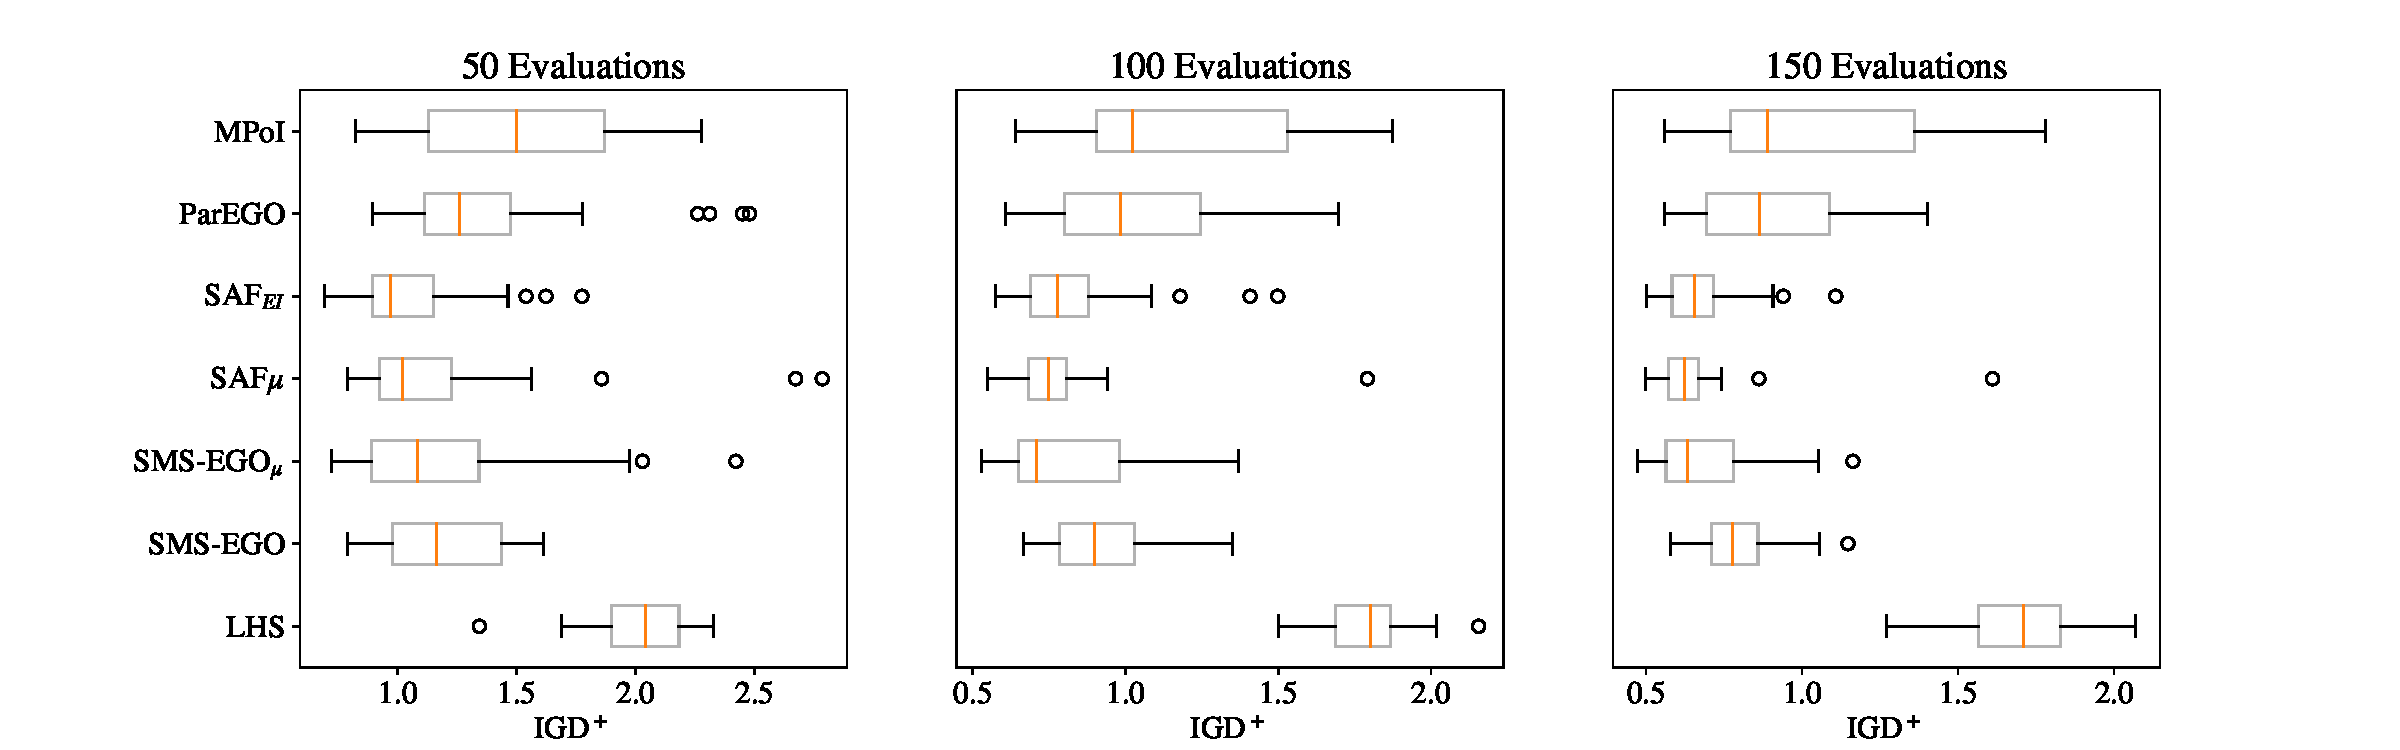
\includegraphics[width=0.8\linewidth]{figures/wfg4_4obj_8dim_igd_boxplot.pdf}
    % \caption{Caption}
\end{subfigure}
    \caption{Box plots showing Dominated Hypervolume and IGD+ over 31 repeats at three stages of the optimisation process.}
\end{figure*}

\clearpage

\begin{figure*}
WFG5\_2M\_6d


\begin{subfigure}[hbt!]{\linewidth}

    \centering
    \includegraphics[width=0.7\linewidth]{figures/wfg5_2obj_6dim_hv_plot.pdf}
    % \caption{Caption}
\end{subfigure}
\begin{subfigure}[h]{\linewidth}
    \centering
    \includegraphics[width=0.7\linewidth]{figures/wfg5_2obj_6dim_igd_plot.pdf}
    % \caption{Caption}
\end{subfigure}
    \caption{Convergence plots showing median Dominated Hypervolume and IGD+ over 31 repeats. IQR shown in shaded region. Dominated hypervolume calculated as a fraction of the maximum possible.}
\vspace{\floatsep}
\begin{subfigure}[t]{\linewidth}
    \centering
    \includegraphics[width=0.8\linewidth]{figures/wfg5_2obj_6dim_hv_boxplot.pdf}
    % \caption{Caption}
\end{subfigure}
\begin{subfigure}[t]{\linewidth}
    \centering
    \includegraphics[width=0.8\linewidth]{figures/wfg5_2obj_6dim_igd_boxplot.pdf}
    % \caption{Caption}
\end{subfigure}
    \caption{Box plots showing Dominated Hypervolume and IGD+ over 31 repeats at three stages of the optimisation process.}
\end{figure*}

\clearpage

\begin{figure*}
WFG5\_3M\_8d


\begin{subfigure}[hbt!]{\linewidth}

    \centering
    \includegraphics[width=0.7\linewidth]{figures/wfg5_3obj_8dim_hv_plot.pdf}
    % \caption{Caption}
\end{subfigure}
\begin{subfigure}[h]{\linewidth}
    \centering
    \includegraphics[width=0.7\linewidth]{figures/wfg5_3obj_8dim_igd_plot.pdf}
    % \caption{Caption}
\end{subfigure}
    \caption{Convergence plots showing median Dominated Hypervolume and IGD+ over 31 repeats. IQR shown in shaded region. Dominated hypervolume calculated as a fraction of the maximum possible.}
\vspace{\floatsep}
\begin{subfigure}[t]{\linewidth}
    \centering
    \includegraphics[width=0.8\linewidth]{figures/wfg5_3obj_8dim_hv_boxplot.pdf}
    % \caption{Caption}
\end{subfigure}
\begin{subfigure}[t]{\linewidth}
    \centering
    \includegraphics[width=0.8\linewidth]{figures/wfg5_3obj_8dim_igd_boxplot.pdf}
    % \caption{Caption}
\end{subfigure}
    \caption{Box plots showing Dominated Hypervolume and IGD+ over 31 repeats at three stages of the optimisation process.}
\end{figure*}
\clearpage

\begin{figure*}
WFG5\_4M\_10d


\begin{subfigure}[hbt!]{\linewidth}

    \centering
    \includegraphics[width=0.7\linewidth]{figures/wfg5_4obj_10dim_hv_plot.pdf}
    % \caption{Caption}
\end{subfigure}
\begin{subfigure}[h]{\linewidth}
    \centering
    \includegraphics[width=0.7\linewidth]{figures/wfg5_4obj_10dim_igd_plot.pdf}
    % \caption{Caption}
\end{subfigure}
    \caption{Convergence plots showing median Dominated Hypervolume and IGD+ over 31 repeats. IQR shown in shaded region. Dominated hypervolume calculated as a fraction of the maximum possible.}
\vspace{\floatsep}
\begin{subfigure}[t]{\linewidth}
    \centering
    \includegraphics[width=0.8\linewidth]{figures/wfg5_4obj_10dim_hv_boxplot.pdf}
    % \caption{Caption}
\end{subfigure}
\begin{subfigure}[t]{\linewidth}
    \centering
    \includegraphics[width=0.8\linewidth]{figures/wfg5_4obj_10dim_igd_boxplot.pdf}
    % \caption{Caption}
\end{subfigure}
    \caption{Box plots showing Dominated Hypervolume and IGD+ over 31 repeats at three stages of the optimisation process.}
\end{figure*}
\clearpage


\begin{figure*}
WFG6\_2M\_10d


\begin{subfigure}[hbt!]{\linewidth}

    \centering
    \includegraphics[width=0.7\linewidth]{figures/wfg6_2obj_10dim_hv_plot.pdf}
    % \caption{Caption}
\end{subfigure}
\begin{subfigure}[h]{\linewidth}
    \centering
    \includegraphics[width=0.7\linewidth]{figures/wfg6_2obj_10dim_igd_plot.pdf}
    % \caption{Caption}
\end{subfigure}
    \caption{Convergence plots showing median Dominated Hypervolume and IGD+ over 31 repeats. IQR shown in shaded region. Dominated hypervolume calculated as a fraction of the maximum possible.}
\vspace{\floatsep}
\begin{subfigure}[t]{\linewidth}
    \centering
    \includegraphics[width=0.8\linewidth]{figures/wfg6_2obj_10dim_hv_boxplot.pdf}
    % \caption{Caption}
\end{subfigure}
\begin{subfigure}[t]{\linewidth}
    \centering
    \includegraphics[width=0.8\linewidth]{figures/wfg6_2obj_10dim_igd_boxplot.pdf}
    % \caption{Caption}
\end{subfigure}
    \caption{Box plots showing Dominated Hypervolume and IGD+ over 31 repeats at three stages of the optimisation process.}
\end{figure*}
\clearpage


\begin{figure*}
WFG6\_3M\_6d


\begin{subfigure}[hbt!]{\linewidth}

    \centering
    \includegraphics[width=0.7\linewidth]{figures/wfg6_3obj_6dim_hv_plot.pdf}
    % \caption{Caption}
\end{subfigure}
\begin{subfigure}[h]{\linewidth}
    \centering
    \includegraphics[width=0.7\linewidth]{figures/wfg6_3obj_6dim_igd_plot.pdf}
    % \caption{Caption}
\end{subfigure}
    \caption{Convergence plots showing median Dominated Hypervolume and IGD+ over 31 repeats. IQR shown in shaded region. Dominated hypervolume calculated as a fraction of the maximum possible.}
\vspace{\floatsep}
\begin{subfigure}[t]{\linewidth}
    \centering
    \includegraphics[width=0.8\linewidth]{figures/wfg6_3obj_6dim_hv_boxplot.pdf}
    % \caption{Caption}
\end{subfigure}
\begin{subfigure}[t]{\linewidth}
    \centering
    \includegraphics[width=0.8\linewidth]{figures/wfg6_3obj_6dim_igd_boxplot.pdf}
    % \caption{Caption}
\end{subfigure}
    \caption{Box plots showing Dominated Hypervolume and IGD+ over 31 repeats at three stages of the optimisation process.}
\end{figure*}
\clearpage

\begin{figure*}
WFG6\_4M\_12d


\begin{subfigure}[hbt!]{\linewidth}

    \centering
    \includegraphics[width=0.7\linewidth]{figures/wfg6_4obj_12dim_hv_plot.pdf}
    % \caption{Caption}
\end{subfigure}
\begin{subfigure}[h]{\linewidth}
    \centering
    \includegraphics[width=0.7\linewidth]{figures/wfg6_4obj_12dim_igd_plot.pdf}
    % \caption{Caption}
\end{subfigure}
    \caption{Convergence plots showing median Dominated Hypervolume and IGD+ over 31 repeats. IQR shown in shaded region. Dominated hypervolume calculated as a fraction of the maximum possible.}
\vspace{\floatsep}
\begin{subfigure}[t]{\linewidth}
    \centering
    \includegraphics[width=0.8\linewidth]{figures/wfg6_4obj_12dim_hv_boxplot.pdf}
    % \caption{Caption}
\end{subfigure}
\begin{subfigure}[t]{\linewidth}
    \centering
    \includegraphics[width=0.8\linewidth]{figures/wfg6_4obj_12dim_igd_boxplot.pdf}
    % \caption{Caption}
\end{subfigure}
    \caption{Box plots showing Dominated Hypervolume and IGD+ over 31 repeats at three stages of the optimisation process.}
\end{figure*}
\clearpage
\end{document}
